\documentclass[letterpaper, 11pt, english, twoside]{MastersDoctoralThesis}

\usepackage[utf8]{inputenc} % Required for inputting international characters
\usepackage[T1]{fontenc} % Output font encoding for international characters

%\usepackage{palatino} % Use the Palatino font by default
\usepackage{mathptmx}% http://ctan.org/pkg/mathptmx
\usepackage{amsmath}
\usepackage{graphicx}
\usepackage[lofdepth,lotdepth]{subfig}
%\usepackage{times}
\usepackage{textcomp}
\usepackage{amssymb}

\usepackage[backend=bibtex,style=authoryear,natbib=true]{biblatex} % Use the bibtex backend with the authoryear citation style (which resembles APA)

\addbibresource{SenResource.bib} % The filename of the bibliography

\usepackage[autostyle=true]{csquotes} % Required to generate language-dependent quotes in the bibliography

%----------------------------------------------------------------------------------------
%	MARGIN SETTINGS
%----------------------------------------------------------------------------------------

\geometry{
	paper=letterpaper, % Change to letterpaper for US letter
	inner=2.5cm, % Inner margin
	outer=3.8cm, % Outer margin
	bindingoffset=2cm, % Binding offset
	top=1.5cm, % Top margin
	bottom=1.5cm, % Bottom margin
	%showframe,% show how the type block is set on the page
}

%----------------------------------------------------------------------------------------
%	THESIS INFORMATION
%----------------------------------------------------------------------------------------

\thesistitle{Universal Real-Time XYZ rectified Reconstruction for RGB-D Cameras}
\university{\href{http://www.uky.edu}{University of Kentucky}} % Your university's name and URL, this is used in the title page and abstract, print it elsewhere with \univname
\author{Sen Li} % Your name, this is used in the title page and abstract, print it elsewhere with \authorname
\supervisor{Daniel L. Lau} % Your supervisor's name, this is used in the title page, print it elsewhere with \supname







\begin{document}
\frontmatter % Use roman page numbering style (i, ii, iii, iv...) for the pre-content pages
\pagestyle{plain} % Default to the plain heading style until the thesis style is called for the body content


%----------------------------------------------------------------------------------------
%	TITLE PAGE
%----------------------------------------------------------------------------------------

\begin{titlepage}
\begin{center}

{\scshape\LARGE \univname\par}\vspace{1.5cm} % University name
\textsc{\Large Master Thesis}\\[0.5cm] % Thesis type

\HRule \\[0.4cm] % Horizontal line
{\huge \bfseries \ttitle\par}\vspace{0.4cm} % Thesis title
\HRule \\[1.5cm] % Horizontal line
 
\begin{minipage}[t]{0.4\textwidth}
\begin{flushleft} \large
\emph{Author:}\\
\href{https://www.linkedin.com/in/sensprouting}{\authorname} % Author name - remove the \href bracket to remove the link
\end{flushleft}
\end{minipage}
\begin{minipage}[t]{0.4\textwidth}
\begin{flushright} \large
\emph{Supervisor:} \\
\href{http://drhalftone.com/}{\supname} % Supervisor name - remove the \href bracket to remove the link  
\end{flushright}
\end{minipage}\\[3cm]
 
 
{\large \today}\\[4cm] % Date
%\includegraphics{Logo} % University/department logo - uncomment to place it
 
\vfill
\end{center}
\end{titlepage}



\tableofcontents
%\listoffigures







%----------------------------------------------------------------------------------------
%	THESIS CONTENT - CHAPTERS
%----------------------------------------------------------------------------------------

\mainmatter % Begin numeric (1,2,3...) page numbering

\pagestyle{thesis} % Return the page headers back to the "thesis" style

% Include the chapters of the thesis as separate files from the Chapters folder
% Uncomment the lines as you write the chapters

% Chapter 1
\chapter{Introduction} % Main chapter title
\label{sens_introduction} % For referencing the chapter elsewhere, use \ref{sens_introduction} 
3D reconstruction aims to reproduce the 3D profile of real objects as accurate as possible, which require accurate world \(X\)/\(Y\)/\(Z\) (noted as \(X^{w}\) /\(Y^{w}\) /\(Z^{w}\)  henceforth) coordinate values in three dimensional space for every single point of a profile. Ever since the Kinect brought low-cost depth cameras into consumer market, with PrimeSense 3D sensing technology as the core depth determination principle for its first generation, great interest has been invigorated into RGB-D sensors. Camera calibration is a necessary part in 3D reconstruction in order to extract metric information from 3D images, i.e., to determine a translation from \(Z^{w}\)  to \(X^{w}\) /\(Y^{w}\)  for every pixel based on its row and column. In the mean time, optical and perspective distortion become a problem that stops from getting a good view. On most wide angle prime lenses and many zoom lenses with relatively short focal lengths,  especially cheap low quality lenses, barrel distortion would typically be present.
\\
\\In this research, a more accurate novel method with precise calibration system is brought in for real-time rectification and 3D reconstruction of universal RGB-D cameras. 
%%%%%%%%%%%%%%%%%%%%%%%%%%%%%%%%%%%%%%%%%%%%%%%%%%%%%%%%%%
%%%%%%%%%%                                                     %%%%%%%%%%%%%%%%%%%%%%%%%%%%%%%%
%%%%%%%%%% 1.1   3D Reconstruction                   %%%%%%%%%%%%%%%%%%%%%%%%
%%%%%%%%%%                                                     %%%%%%%%%%%%%%%%%%%%%%%%
%%%%%%%%%%%%%%%%%%%%%%%%%%%%%%%%%%%%%%%%%%%%%%%%%%%%%%%%%%%%
\section{3D Reconstruction}
%
\begin{figure}[h]
\centering
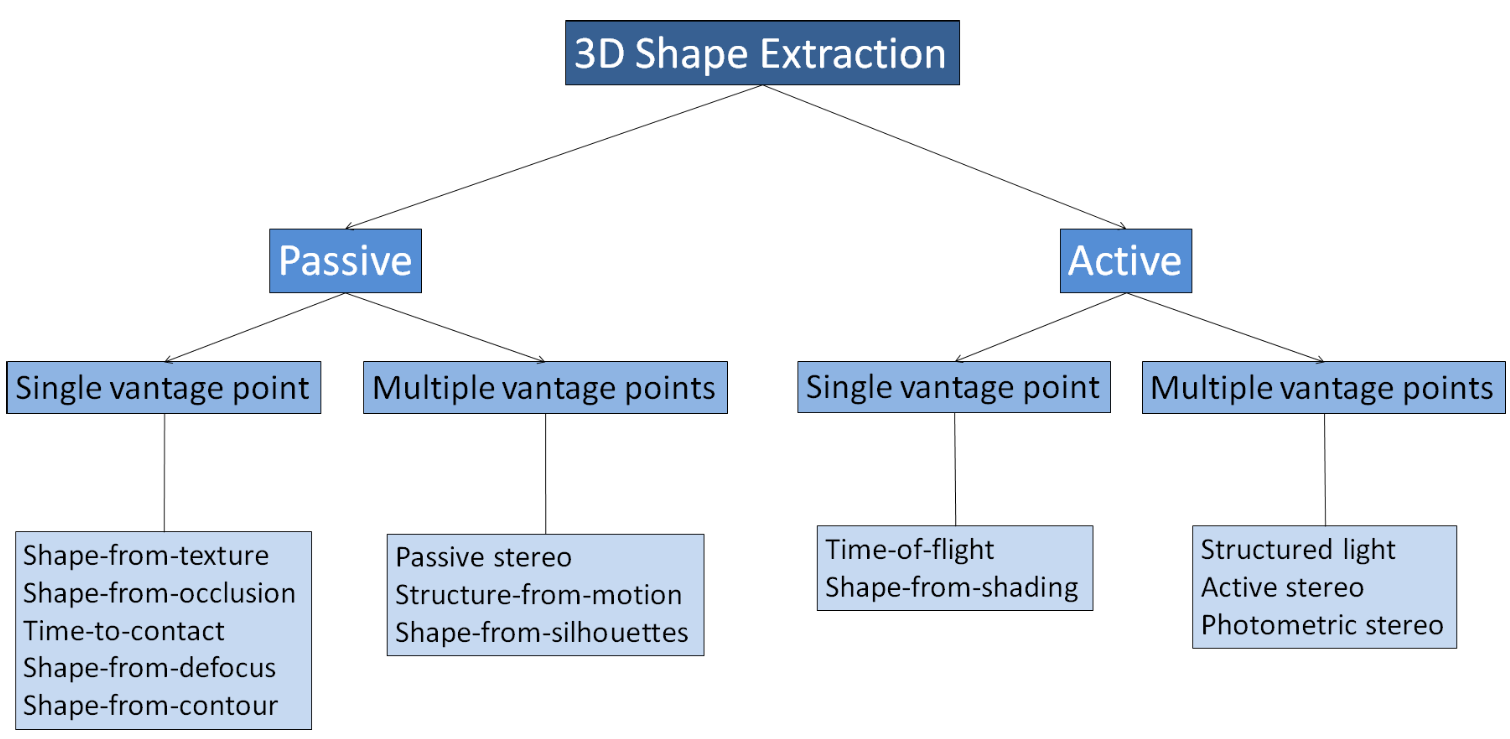
\includegraphics[width=\textwidth]{3DImagingBranchTree}
\caption{ 3D profile acquisition Taxonomy}
\label{3DImagingTaxonomy}
\end{figure}%
\par%
Three dimensional (3D) profile measurement technologies have been developed by various means, as summarized by Curless and Seitz [1], % B. Curless and S. Seitz, \3d photography," ACM Siggraph '00 Course Notes, Course No. 19 (2000).
among which the non-contact optical methods are widely applied into reality as consumer RGB-D camera. Traditionally, with Pinhole camera model, as the basics of camera calibration, to supply the translation from \(Z^{w}\)  to \(X^{w}\) /\(Y^{w}\) , the core procedure of 3D Reconstruction falls on the determination of per-pixel depth to serve as \(Z^{w}\) .\par%
%
Within the non-contact optical category, as well as 3D reconstruction using multiple images, there are two levels of distinctions[2],
% 3D Reconstruction from Multiple Images.pdf
 as shown in the 3D profile acquisition taxonomy diagram is given in Figure \ref{3DImagingTaxonomy}.
 %
 \\\\The first distinction: active methods and passive methods. Their classifications are decided by the control of light sources. Active methods need special light sources control as part of the strategy to get 3D information, while on the other hand, passive techniques could work with whichever reasonable available ambient light. With a special known illumination offering more information to simplify some of the steps for 3D information acquiring process, active methods tend to be computationally less demanding. Both of the famous consumer PrimeSense and KinectV2 3D cameras, which are calibrated by the new proposed approach, are using active methods.
\\\\The second distinction: single-vantage points methods and multi-vantage points methods. The second distinction is determined by the number of vantage points. With a single vantage system, reconstruction is done based on single view point. In the case that there are multiple viewing or illumination components, all of them would be positioned very close to each other so that they could ideally coincide. For multi-vantage points methods, several viewpoints, with possible controlled illumination source positions, are involved. As contrast with the single-vantage points methods, the multi-vantage systems need the different components to be positioned far enough from each other. 
\\ \\
Among the above non-contact optical methods, structured-light and time-of-flight methods are of the most practical importance.
As will be discussed shortly, the PrimeSense technology and SeikowaveLCG camera use Stuctured light methods, and the KniectV2 camera uses Time-of Flight. 
\\
\\\textbf{Structured Light}\\\\
Structured light (SL) based techniques are famous for its fast speed. It is composed of one camera and one light pattern projector[3]. %Real-time 3-D Reconstruction by Means of Structured Light Illumination
The projector projects a series of special known patterns onto a target, and the camera captures the corresponding images, which contain special information corresponded to the patterns from the projector. A decoding algorithm would be used to extract world coordinate information of the target object from the captured images, by analyzing the relationship among the camera, the projector and the target object using triangulation.\\
\\
Being after accuracy, the most important issue for structured light method comes to the question of, how to design the projected patterns. In other words, how to design the coding algorithm and its corresponding decoding strategy will decide the final quality of the reconstructed 3D profile. Various classified SL pattern strategies have been proposed, and are still being studied.
\\
\subsection{PrimeSense Structured Light}
The PrimeSense 3D camera uses an infrared projector to project an infrared speckle pattern onto a target 
% RGBD-intro.pdf/   Consumer RGBD Cameras and their Applications
, as shown in figure \ref{PrimeSenseInfraredPattern},\par%Figure1 in the pdf named above
%
\begin{figure}[h]
\centering
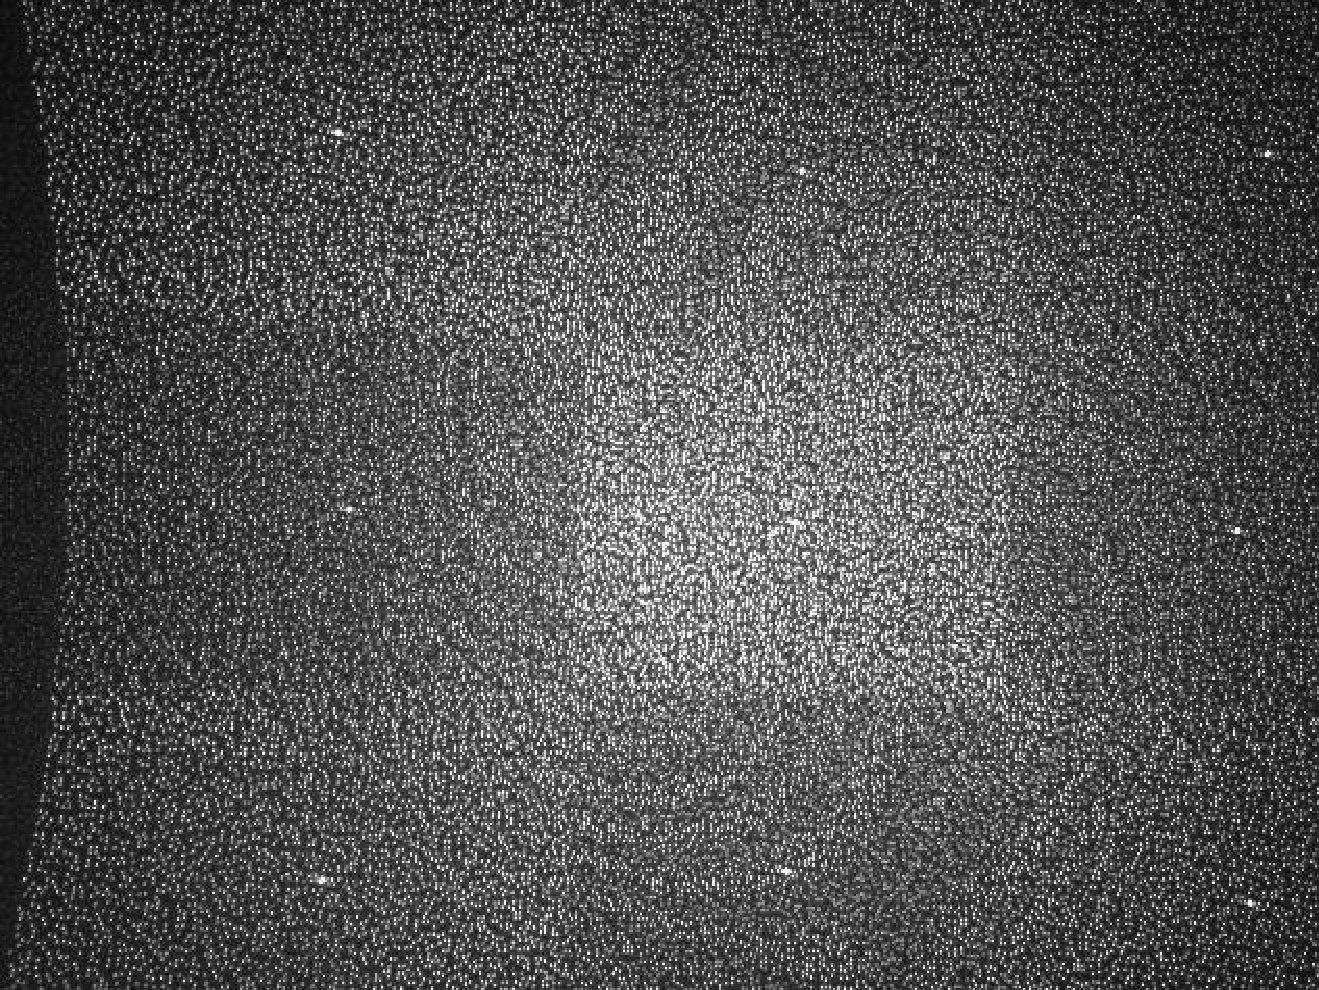
\includegraphics[width=0.8\textwidth]{PrimeSenseInfraredPattern}
\caption{PrimeSense SL Infrared Pattern}
\label{PrimeSenseInfraredPattern}
\end{figure}%
%
and an infrared camera to capture images of the target. By comparing part by part to reference patterns, that were captured previously at known depths and stored in the device, the per-pixel depth could be looked up based on the reference pattern that the projected pattern matches best. 
\\\\
After the per-pixel depth data determined from the infrared sensor, the next step would be to correlate to a calibrated RGB data, which will generate a popular unified representation of target's profile: point cloud, a collection of points with \(XYZ\) 3D coordinates and RGB color data. What's more, the surface normals of the target's profile are also stored in every single point of the point cloud data. 
\\
\subsection{SeikowaveLCG SL Phase Measuring Profilometry}
SeikowaveLCG 3D camera consists of a Charge-Coupled Device (CCD) camera and a Digital Micro-mirror Device (DMD) projector. 2D image pattern strategies are always preferred for a fast scan if a is involved. 
[4]%J. Salvi, J. Pages, and J. Batlle, \Pattern codication strategies in structured light systems," Pattern Recognition 37, 827{849 (2004).
 [5] %  ''Novel method for structured light system calibration'' SongZhang
And the multi-shot pattern Phase Measuring Profilometry (PMP) strategy was used for its properties of robust and accuracy.
With PMP information encoded in the structured light pattern projected onto the target, the CCD camera could capture a series of images that contains PMP informatio. Triangulation analyzing could be used to extract the 3D world coordinates for each points of the target profile, by a determination of the relationships among CCD camera, DMD projector, and the target object. A system configuration of PMP application is given in figure \ref{SLPMPConfiguration}.\par%
%
\begin{figure}[h]
\centering
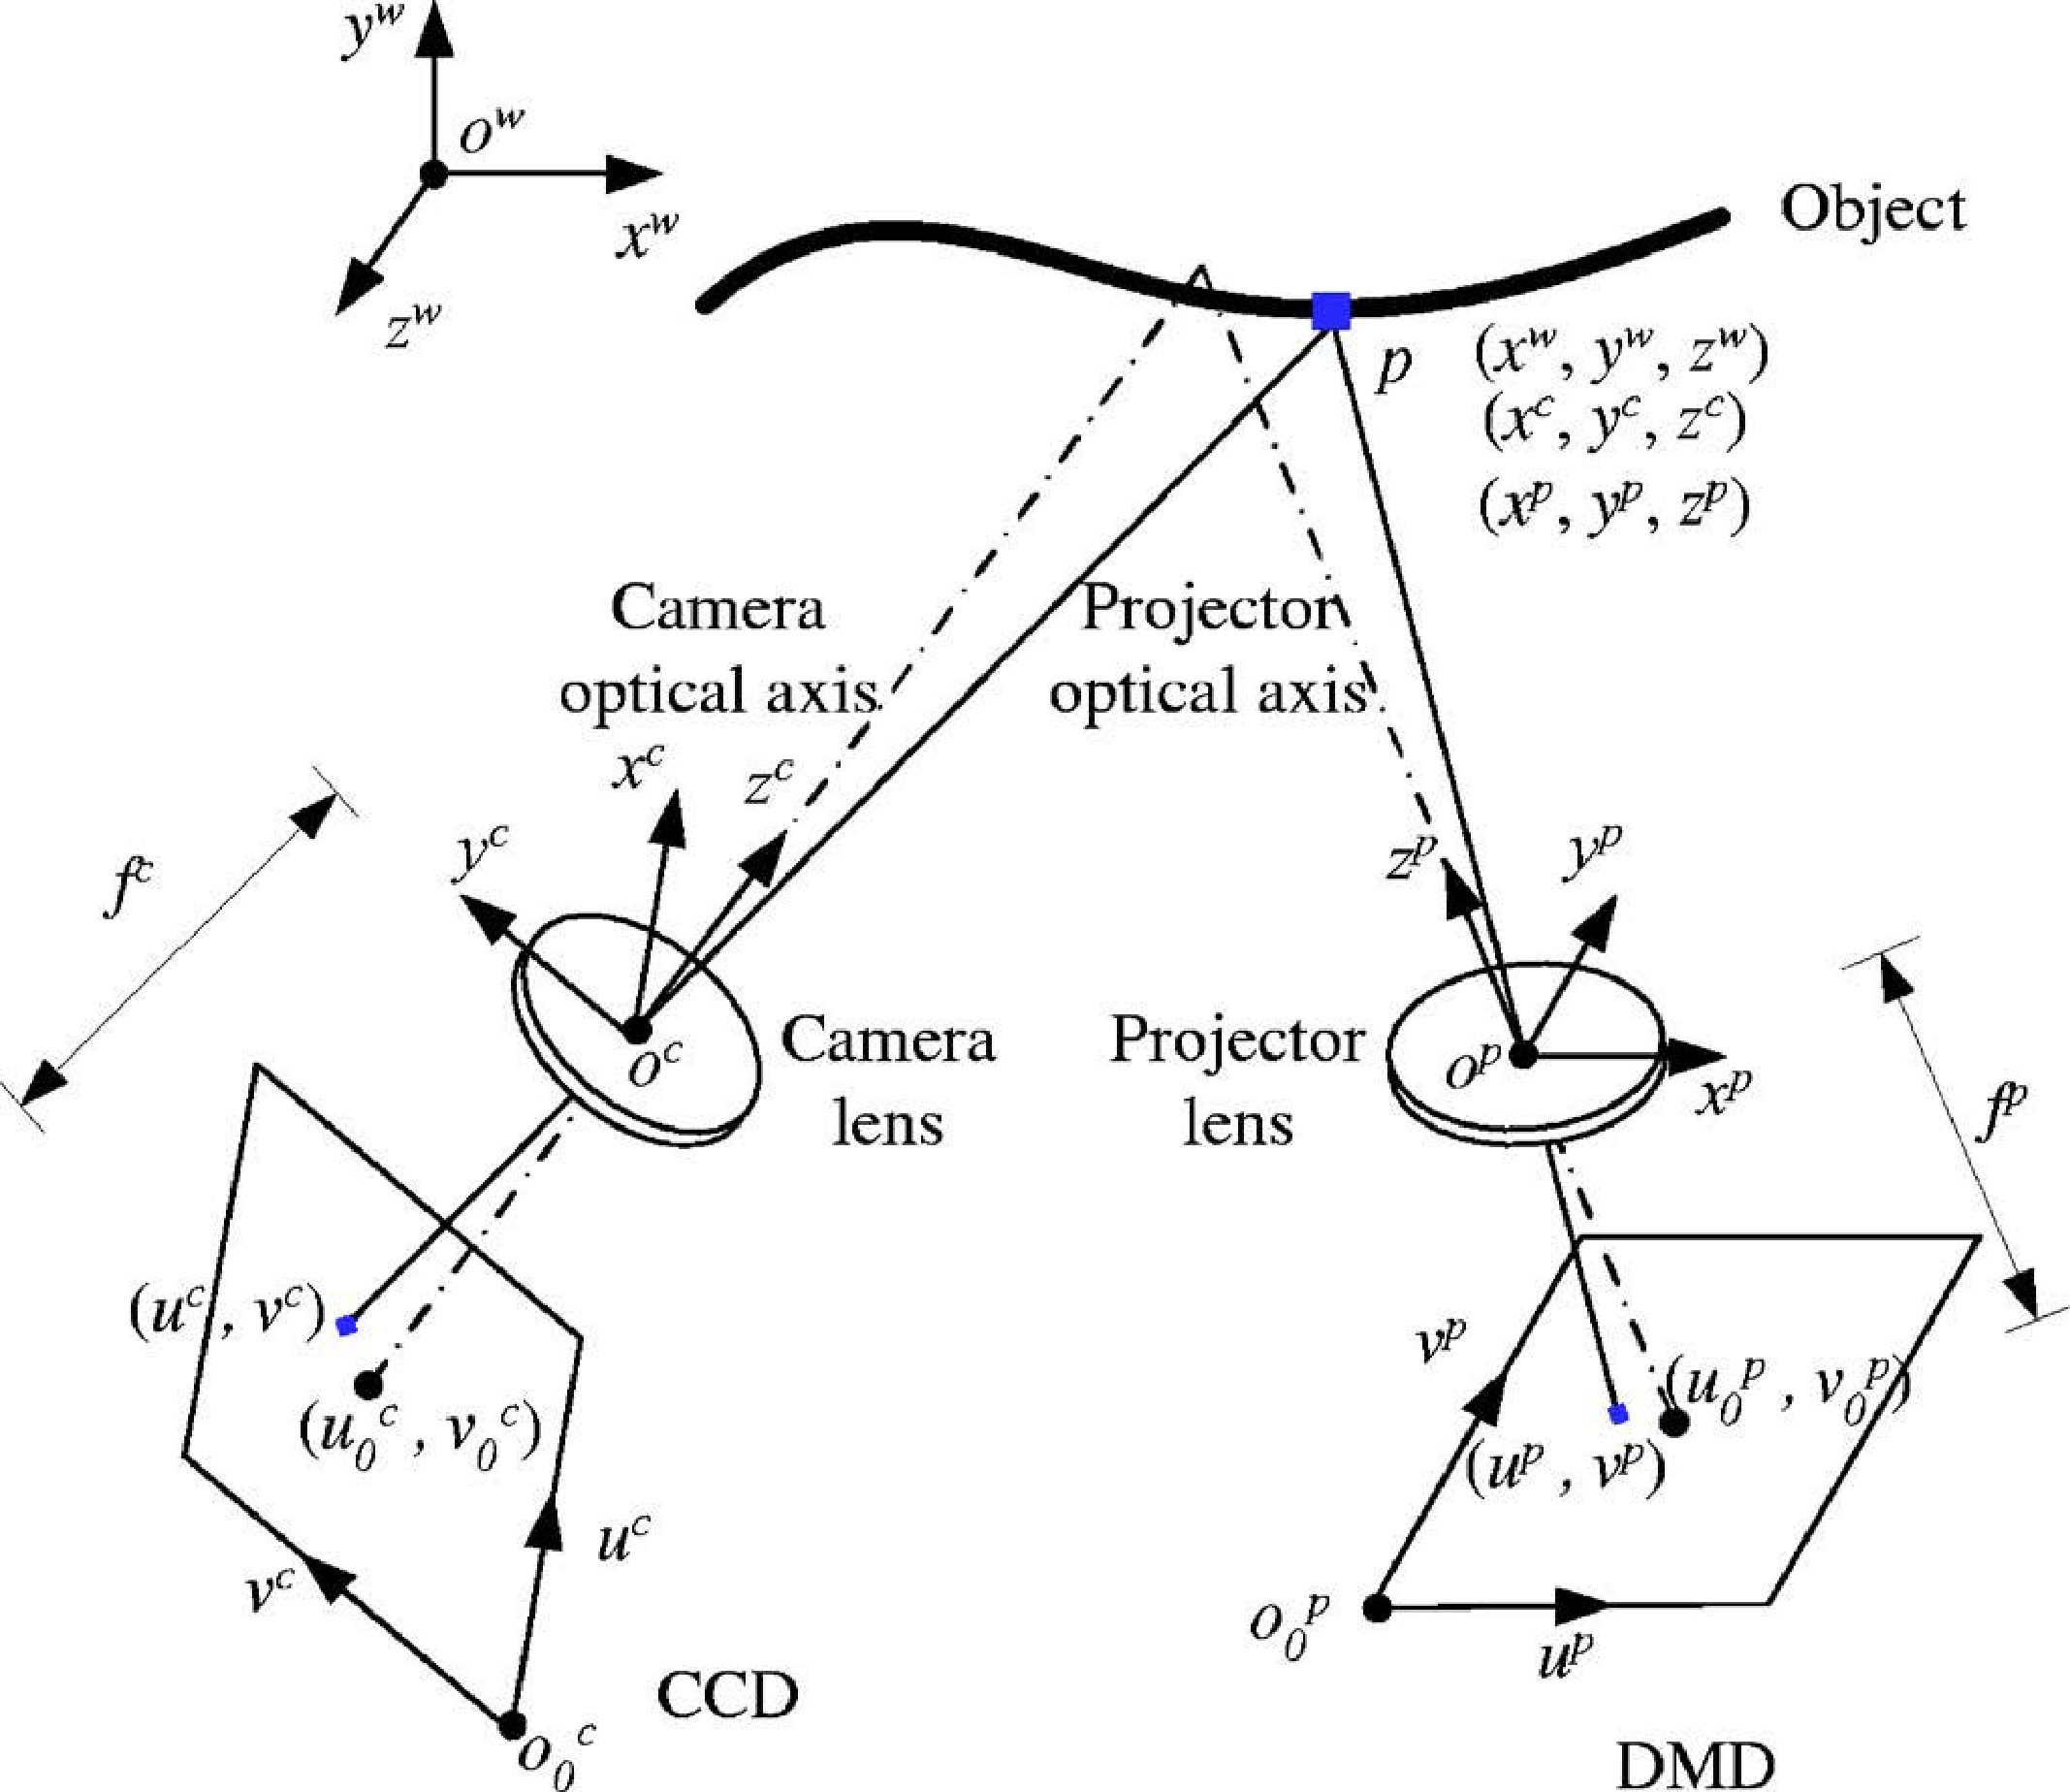
\includegraphics[width=0.7\textwidth]{SLPMPConfiguration}
\caption{SL PMP based Configuration Diagram}
\label{SLPMPConfiguration}
\end{figure}%
%
PMP method uses either vertical or horizontal sinusoid patterns, which could be described as:

 \begin{equation}
%
I^p_n(x^p, \, y^p) %
= A^p(x^p, \, y^p) + B^p(x^p, \, y^p)Cos(2\pi fy^p - \frac{2\pi n}{N})
%
\end{equation}%
%
where \((x^p, \, y^p)\) denotes the coordinates of every single pixel in the projector, \(I^p_n\) denotes the intensity of the corresponding pixels, \(A^p\) and \(B^p\) are constants, \(f\) is the frequency of sine wave. The subscript \(n\) represents the index of phase shift, while capital \(N\) is the total number of phase shift.\par%
%
%
 \begin{figure}[h]
%\centering
\hspace*{-2cm} 
\subfloat[Pattern 0][1]{

\includegraphics[width=0.3\textwidth]{Pattern0}
\label{fig:subfig1}}
\subfloat[Pattern 1][2]{

\includegraphics[width=0.3\textwidth]{Pattern1}
\label{fig:subfig2}}
\subfloat[Pattern 2][3]{

\includegraphics[width=0.3\textwidth]{Pattern2}
\label{fig:subfig3}}
%\qquad
\subfloat[Pattern 3][4]{

\includegraphics[width=0.3\textwidth]{Pattern3}
\label{fig:subfig4}}
\caption{PMP base frequency patterns}
\label{PMPFrequencyPatterns}
\end{figure}%
%
%
Figure \ref{PMPFrequencyPatterns} shows a group of sine wave patterns, where the number of total phase shift \(N = 4\) and frequency \(f = 1\). From viewpoint of the camera, the sinusoid patterns is distorted by the target surface topology, so that the captured images could be expressed as 

 \begin{equation}
%
I^c_n(x^c, \, y^c) %
= A^c(x^c, \, y^c) + B^c(x^c, \, y^c)Cos[\phi(x^c,\, y^c) - \frac{2\pi n}{N}]
%
\end{equation}%
%
where\((x^c, \, y^c)\) denotes the coordinates of every single pixel in the camera, and the term \(\phi(x^c,\, y^c)\) represents the corresponding phase value, which could be computed as follows [6]\par
 % Very High Resolution 3-D surface Scanning Using Multi-Frequency Phase Measuring Profilometry
 \begin{equation}
%
\phi(x^c,\, y^c) %
= arctan\Bigg[\frac{\sum^N_{n=1}I(x^c,\,y^c)Sin(2\pi n / N)}{\sum^N_{n=1}I(x^c,\,y^c)Cos(2\pi n / N)} \Bigg]
%
\end{equation}
%
%
After the camera term  \(\phi(x^c,\, y^c)\)  for every single pixel is computed, the corresponding projector coordinate \(y^p\) could be derived through equation\par

\begin{equation}
%
y^p %
= \phi(x^c,\, y^c) / (2\pi f)
%
\end{equation}%
%
With the knowledge of \(y^p\), the perspective information between camera and projector is the last step to go for applying triangulation analysis to extract world coordinates. Based on pinhole camera model, the perspective matrices for both of the CCD camera and DMD projector, as will be derived later in section \ref{sectionPinholeCamera} equation \ref{genericPerspectivePinholeMatrix}, are written as [7]\par
% J. Li, L. G. Hassebrook, and C. Guan, \Optimized two-frequency phasemeasuring-prolometry light-sensor temporal-noise sensitivity," Journal of the Optical Society of America A 20, 106{115 (2003).

\begin{equation}
%
M^c %
= \begin{bmatrix} 
m^c_{11} & m^c_{12} & m^c_{13} & m^c_{14} \\
m^c_{21} & m^c_{22} & m^c_{23} & m^c_{24} \\
m^c_{31} & m^c_{32} & m^c_{33} & m^c_{34} \\
\end{bmatrix}%
%
%\label{genericPerspectivePinholeMatrix}
\end{equation}%
%
and 

\begin{equation}
%
M^p %
= \begin{bmatrix} 
m^p_{11} & m^p_{12} & m^p_{13} & m^p_{14} \\
m^p_{21} & m^p_{22} & m^p_{23} & m^p_{24} \\
m^p_{31} & m^p_{32} & m^p_{33} & m^p_{34} \\
\end{bmatrix}%
%
%\label{genericPerspectivePinholeMatrix}
\end{equation}%
%
The mapping from 3D world coordinates to 2D camera coordinates are given by\par

\begin{equation}
%
x^c %
= \frac%
{m^c_{11}X^w + m^c_{12}Y^w + m^c_{13}Z^w + m^c_{14}}%
{m^c_{31}X^w + m^c_{32}Y^w + m^c_{33}Z^w + m^c_{34}}
%
\label{cameraXmapping}
\end{equation}%
%
%
\begin{equation}
%
y^c %
= \frac%
{m^c_{21}X^w + m^c_{22}Y^w + m^c_{23}Z^w + m^c_{24}}%
{m^c_{31}X^w + m^c_{32}Y^w + m^c_{33}Z^w + m^c_{34}}
%
\label{cameraYmapping}
\end{equation}%
%
%
Likewise, the translation from 3D world coordinates to 2D projector coordinates are given by\par
\begin{equation}
%
x^p %
= \frac%
{m^p_{11}X^w + m^p_{12}Y^w + m^p_{13}Z^w + m^p_{14}}%
{m^p_{31}X^w + m^p_{32}Y^w + m^p_{33}Z^w + m^p_{34}}
%
\label{projectorXmapping}
\end{equation}%
%
\begin{equation}
%
y^p %
= \frac%
{m^p_{21}X^w + m^p_{22}Y^w + m^p_{23}Z^w + m^p_{24}}%
{m^p_{31}X^w + m^p_{32}Y^w + m^p_{33}Z^w + m^p_{34}}
%
\label{projectorYmapping}
\end{equation}%
%
%
Since three out of four equations \ref{cameraXmapping} \texttildelow \,\ref{projectorYmapping} are enough to solve \(X^{w}\),  \(Y^{w}\),  and \(Z^{w}\), and \(y^p\) is already calculated, the 3D world coordinates \(X^{w}\)/\(Y^{w}\)/\(Z^{w}\)  could be derived from Eqs  \ref{cameraXmapping},  \ref{cameraYmapping}, and \ref{projectorYmapping}\par%
%
\begin{equation}
\hspace*{-0.3cm} 
%
\left[ \begin{array}{c} X^w\\ Y^w\\ Z^w\end{array} \right] %
= %
\begin{bmatrix} %
m^c_{11} - m^c_{31}x^c, &m^c_{12} - m^c_{32}x^c, &m^c_{13} - m^c_{33}x^c \\%
m^c_{21} - m^c_{31}y^c, &m^c_{22} - m^c_{32}y^c, &m^c_{23} - m^c_{33}y^c \\%
m^p_{21} - m^p_{31}y^p, &m^p_{22} - m^p_{32}y^p, &m^p_{23} - m^p_{33}y^p %
\end{bmatrix} ^{-1} %
\left[ \begin{array}{c}%
m^c_{34}y^c - m^c_{14}\\%
m^c_{34}y^c - m^c_{24}\\%
m^p_{34}y^p - m^p_{24}%
\end{array} \right]
%
\end{equation}%
\\\\%
%
\subsection{Time of Flight (KinectV2)}
Based on known speed of light, Time-of-Flight (ToF) camera resolves distance by measuring the time cost of a special light signal traveling between the camera and target for every single point. KinectV2 is one of the practical consumer 3D camera that applied the technology of ToF. Using the active modulated infrared source light together with a low-cost CMOS pixel array, KinectV2 realize its an attractive solution that owns compact construction, high accuracy and up to 30 fps frame-rate.\par%
%
%
\begin{figure}[h]
\centering
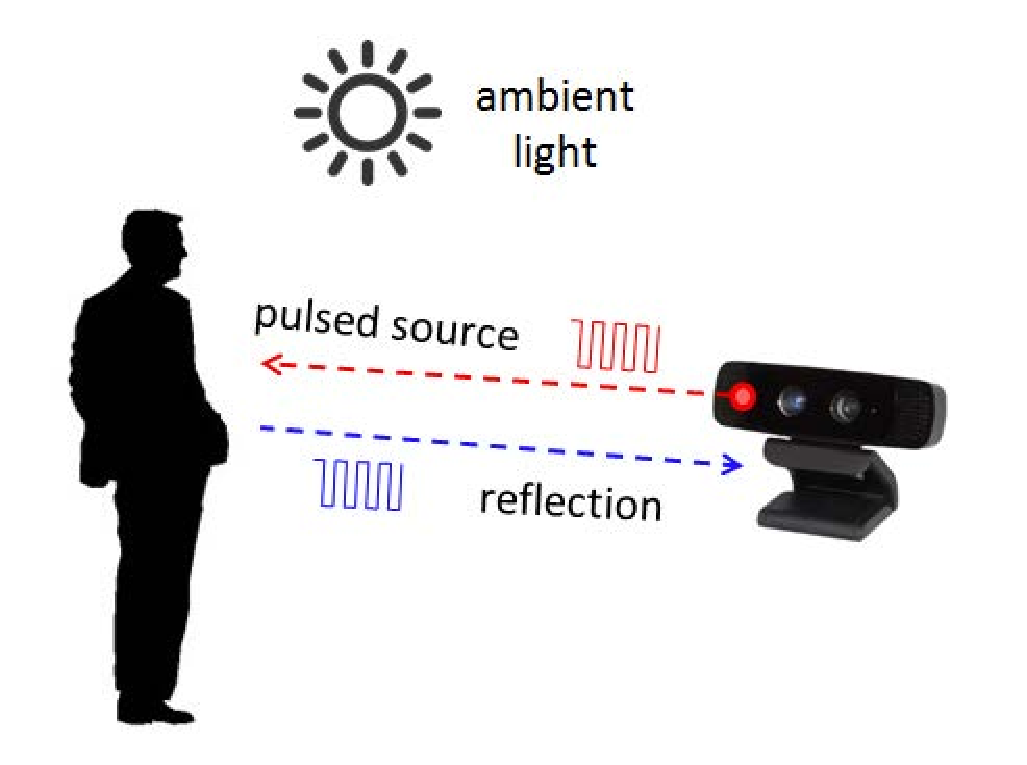
\includegraphics[width=0.7\textwidth]{timeOfFlight}
\caption{3D time-of-flight camera operation}
\label{timeOfFlight}
\end{figure}%
%
The variable that ToF camera measures is the phase shift between the illumination and reflection, which will be translated to distance [8]. % Texas Instruments Time-of-Flight Camera -An Introduction    Larray Li
To detect the phase shifts, light source is pulsed or modulated by a continuous wave, typically a sinusoid or square wave.
As figure \ref{timeOfFlight} shows, the ToF camera illumination is typically from a LED or a solid-state laser operating in the near-infrared range invisible to human eyes. A camera working in the same spectrum captures the reflected light and converts photonic energy to electrical signal, which contains distance (depth) information.
\\\\
The distance measured for every single pixel is saved into a 2D addressable array, which results in a depth map. KinectV2 has a depth map of 512 * 424 unsigned short data collections, which could be finally rendered, together with corresponded RGB stream,  into a tree dimensional space point cloud.
%%%%%%%%%%%%%%%%%%%%%%%%%%%%%%%%%%%%%%%%%%%%%%%%%%%%%%%%%%
%%%%%%%%%%                                                     %%%%%%%%%%%%%%%%%%%%%%%%%%%%%%%%
%%%%%%%%%%  1.2   Traditional RGB-D camera calibration                   %%%%%%%%%%%%%%%%%%%%%%%%
%%%%%%%%%%                                                     %%%%%%%%%%%%%%%%%%%%%%%%
%%%%%%%%%%%%%%%%%%%%%%%%%%%%%%%%%%%%%%%%%%%%%%%%%%%%%%%%%%%%
\section{Traditional RGB-D camera calibration} % (specially with cheap low quality lenses)
\label{sens_TraditionalCalibration} % For referencing the chapter elsewhere, use \ref{sens_TraditionalCalibration} 
Traditionally, camera calibration consists of two parts: ideal pinhole camera model calibration, and lens distortion correction. The pinhole camera model works as an simple algorithm in 3D computer vision to describe a mapping from the 3D world coordinates to camera image row and column, thereby giving a translation method from \(Z^{w}\) to \(X^{w}\)  and \(Y^{w}\)  for every single pixel. It works decently only for ideal pinhole cameras that have no lens, whereas real cameras need extra modifications and supplementations. In order to accurately solve the non-linear distortions problem for a real camera, the second part radial and tangential lens distortion must be considered.\\\par

\subsection{Pinhole Camera Model}
\label{sectionPinholeCamera}
%%
Figure \ref{PinholeCameraModel} shows the basic diagram of a pinhole camera model with a reflected image plane for friendly intuition
[9].% Short on camera geometry and camera calibration/ Maria Magnusson
From this model, the mapping between 3D space world coordinate and the image plane row and column could be separated into two parts of transformations. The first part is the transformation between world coordinates system \(X\)/\(Y\)/\(Z\) and camera coordinate system \(U\)/\(V\)/\(W\) , which forms a 4x4 perspective transformation matrix (\textbf{extrinsic calibration}) that works for 3D rotation and translation. And the second part is the mapping between 3D camera coordinates system \(U\)/\(V\)/\(W\) and 2D image plane coordinates  \(u\)/\(v\), which forms a 3x3 perspective transformation matrix (\textbf{intrinsic calibration}) that works for not only the rescaling between camera coordinates and virtual ideal image coordinates, but also for translating and skewing between the virtual ideal image plane and real image plane.  \\\\\par

\begin{figure}[h]
\centering
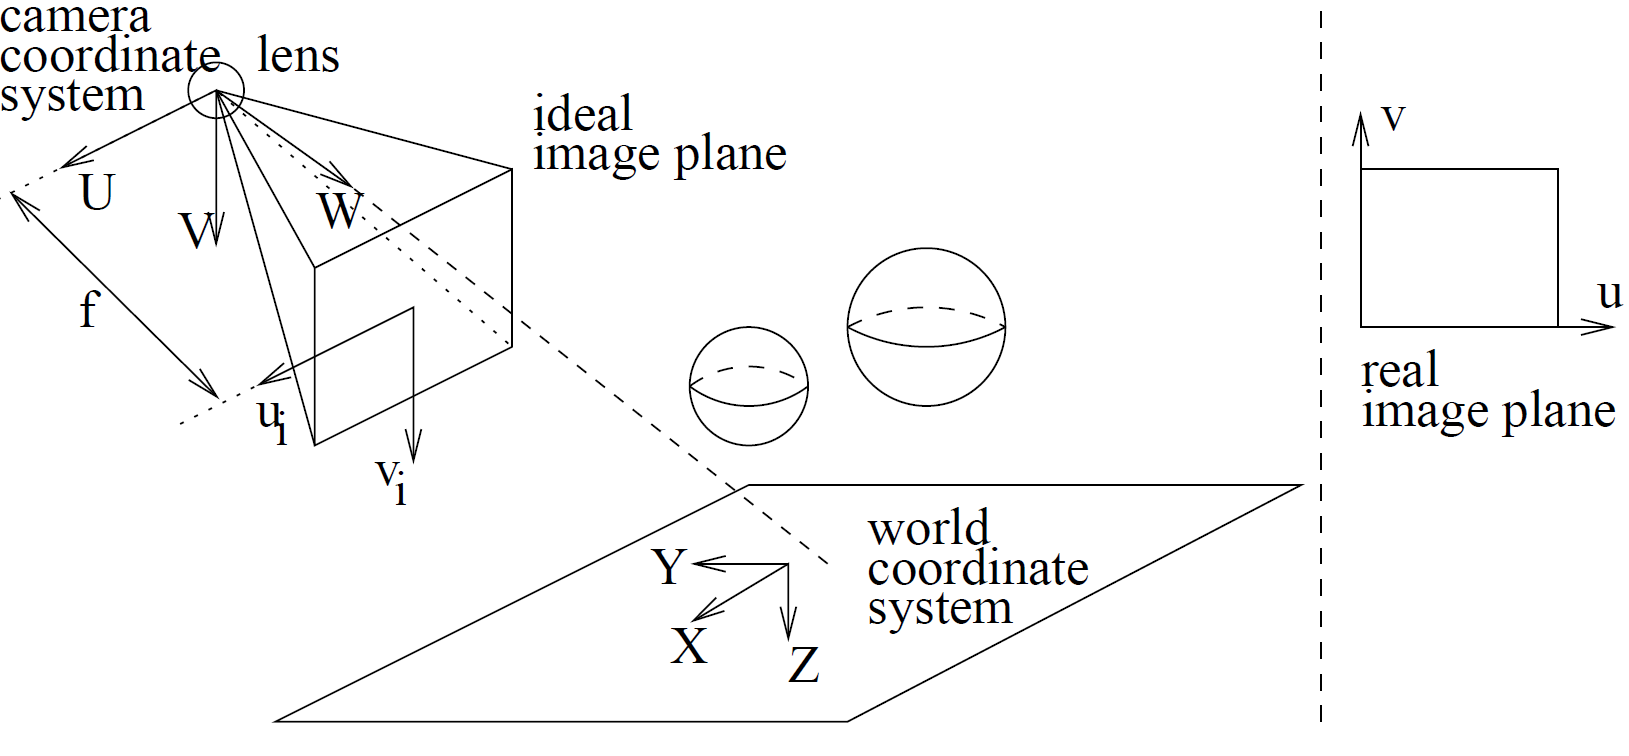
\includegraphics[width=\textwidth]{PinholeCameraModel}
\caption{The pinhole camera model}
\label{PinholeCameraModel}
\end{figure}%
%
\textbf{Extrinsic Calibration}\\
Without any camera parameters, the extrinsic calibration formula could be written, through homogeneous coordinates, as

\begin{equation}
%
\left[ \begin{array}{c} U \\ V \\ W \\ 1 \end{array} \right] %
= %
\begin{bmatrix} R & T \\ 0 & 1 \end{bmatrix} \times \left[ \begin{array}{c} X^w \\ Y^w \\ Z^w \\ 1 \end{array} \right]
%
\end{equation}%
%
or for simplicity,
\begin{equation}
%
\left[ \begin{array}{c} U \\ V \\ W \end{array} \right] %
= %
\begin{bmatrix} R & T \end{bmatrix} \cdot \left[ \begin{array}{c} X^w \\ Y^w \\ Z^w \end{array} \right]
\label{extrinsicTransform}
%
\end{equation}%
%
where \((U, V, W)^T\) are the camera coordinates, and the transformation matrix component \([R\)  \(T]\), which is part of the 4x4 perspective matrix, is modelling rotation and translation , written as

\begin{equation}
%
\left[ \begin{array}{cc} R & T \end{array} \right] %
= %
\begin{bmatrix}
 r_{11} & r_{12} & r_{13} & t_1 \\
 r_{21} & r_{22} & r_{23} & t_2 \\
 r_{31} & r_{32} & r_{33} & t_3
\end{bmatrix}
%
\end{equation}
\\\par
%
%
\textbf{Intrinsic Calibration}\\
Intrinsic Calibration could be separated into two sections. The first section is to rescale from camera coordinates to virtual ideal image coordinates. For a easier integration of two sections, the first section's formula is given through both of 2D coordinates to homogeneous coordinates.\par
%
\quad\quad2D coordinates:%
\begin{equation}
%
W \left[ \begin{array}{c} u_i \\ v_i  \end{array} \right] %
= f %
\left[ \begin{array}{c} U \\ V \end{array} \right]%
%
\end{equation}

\quad\quad Homogeneous coordinates:\par
\begin{equation}
%
W \left[ \begin{array}{c} u_i \\ v_i \\ 1 \end{array} \right] %
= %
\left[ \begin{array}{c} fU \\ fV \\ W \end{array} \right]%
=  \begin{bmatrix} f & 0 & 0 \\ 0 & f & 0 \\ 0 & 0 & 1 \end{bmatrix} \cdot %
\left[ \begin{array}{c} U \\ V \\ W \end{array} \right]%
\label{section_1}
\end{equation}%
\\\par
%
The second section is for translating and skewing between the virtual ideal image plane \(u_i\)/\(v_i\) and real image plane \(u_r\)/\(v_r\),  %

\begin{equation}
%
\left[ \begin{array}{c} u_r \\ v_r \\ 1 \end{array} \right] %
=  \begin{bmatrix} s_u & s_\theta & u_0 \\ 0 & s_v & v_0 \\ 0 & 0 & 1 \end{bmatrix} \cdot %
\left[ \begin{array}{c} u_i \\ v_i \\ 1 \end{array} \right]%
\label{section_2}
\end{equation}%
where \((u_0, v_0)\) denotes the optical center (or principal point), \([s_u, s_v]\) are skew coefficients in pixels along \(u\) and  \(v\) axes , and  \(s_\theta\) is an skewed angle generated by \(s_u\) and  \(s_v\). To combine equation \ref{section_1} and equation \ref{section_2}, we could get %

\begin{equation}
%
W \left[ \begin{array}{c} u_r \\ v_r \\ 1 \end{array} \right] %
=  \begin{bmatrix} s_u & s_\theta & u_0 \\ 0 & s_v & v_0 \\ 0 & 0 & 1 \end{bmatrix} \cdot%
 \begin{bmatrix} f & 0 & 0 \\ 0 & f & 0 \\ 0 & 0 & 1 \end{bmatrix} \cdot %
\left[ \begin{array}{c} U \\ V \\ W \end{array} \right]%
=  \begin{bmatrix} f_u & s & u_0 \\ 0 & f_v & v_0 \\ 0 & 0 & 1 \end{bmatrix} \cdot%
\left[ \begin{array}{c} U \\ V \\ W \end{array} \right]%
%
\label{intrinsicTransform}
\end{equation}%
%
where \([f_u,\, f_v]\) denote focal lengths in pixels along \(u\) and \(v\) after skewing, and \(s\) is a new skew coefficient after combination.\\\par%
%
\textbf{Generic Perspective Matrix of the Pinhole Camera Model}\par%
After both of the extrinsic and intrinsic transformation matrices have been derived, the generalization formula of the pinhole camera model could be derived, combining equation \ref{extrinsicTransform} and \ref{intrinsicTransform}, as

\begin{equation}
%
k \left[ \begin{array}{c} u_r \\ v_r \\ 1 \end{array} \right] %
=  \begin{bmatrix} f_u & s & u_0 \\ 0 & f_v & v_0 \\ 0 & 0 & 1 \end{bmatrix} \cdot%
\begin{bmatrix} R & T \end{bmatrix} \cdot \left[ \begin{array}{c} X^w \\ Y^w \\ Z^w \end{array} \right]%
=  C \cdot \left[ \begin{array}{c} X^w \\ Y^w \\ Z^w \end{array} \right]%
%
\end{equation}%
%
where \(W\) on the left side has been replaced by \(k\) to be a more general proportion coefficient, and a combined matrix can be expressed as
\begin{equation}
%
C %
=  \begin{bmatrix} f_u & s & u_0 \\ 0 & f_v & v_0 \\ 0 & 0 & 1 \end{bmatrix} \cdot%
\begin{bmatrix} R & T \end{bmatrix}%
= \begin{bmatrix} 
m_{11} & m_{12} & m_{13} & m_{14} \\
m_{21} & m_{22} & m_{23} & m_{24} \\
m_{31} & m_{32} & m_{33} & m_{34} \\
\end{bmatrix}%
%
\label{genericPerspectivePinholeMatrix}
\end{equation}%
%
The final 3x4 matrix C is considered as the generic perspective transformation matrix of a pinhole camera model, which gives a mapping between the 3D world coordinates and 2D real image coordinates.\par

\subsection{Lens distortion}
Lens distortion could be classified into two groups [10] : radial distortion, and tangential distortion.\par
%Z. Zhang, "Camera Calibration",   Chapter 2, pages 4-43, in G. Medioni and S.B. Kang, eds., Emergin Topics in Computer Vision, Prentice Hall Professional Technical Reference, 2004. .\par
%
Imperfect lens shape causes light rays bending more near the edges of a lens than they do at its optical center. The smaller the lens, the greater the distortion. Barrel distortions happen commonly on wide angle lenses, where the field of view of the lens is much wider than the size of the image sensor.\par%
Improper lens assembly will lead to tangential distortion, which occurs when the lens and the image plane are not parallel.\\\par
%
The lens distortion can be expressed as power series in radial distance \(r = \sqrt{x^2 + y^2}\):
\begin{equation}
%
\begin{aligned}
x_{distorted} =  x (1 + k_1 r^2 + k_2 r^4 + k_3 r^6) + [p_1 (r^2 + 2 x^2) + 2 p_2 xy] %
\\%
y_{distorted} =  y (1 + k_1 r^2 + k_2 r^4 + k_3 r^6) + [p_2 (r^2 + 2 y^2) + 2 p_1 xy]
\end{aligned}
\label{lensDistortion}
%
\end{equation}%

where higher order parameters are omitted for being negligible; \((x_{distorted}, \, y_{distorted})\) denote the distorted points, \((x, \, y)\) denote the undistorted pixel locations, \(k_i\)'s are coefficients of radial distortion, and \(p_j\)'s are coefficients of tangential distortion.\par
%
%%%%%%%%%%%%%%%%%%%%%%%%%%%%%%%%%%%%%%%%%%%%%%%%%%%%%%%
%%%%%%%%%%                                                     %%%%%%%%%%%%%%%%%%%%%%%%%%%
%%%%%%%%%%  1.3   Contributions of this thesis             %%%%%%%%%%%%%%%%%%%%%%%%
%%%%%%%%%%                                                     %%%%%%%%%%%%%%%%%%%%%%%%
%%%%%%%%%%%%%%%%%%%%%%%%%%%%%%%%%%%%%%%%%%%%%%%%%%%%%%%
\section{Contributions of this thesis}

%	****  Fourth order (abandon pinhole camera model) **********\\
%	****  Depth Rectification ************\\
%	****  Real-Time Reconstruction  ******\\
%	****  accurate calibration system *******\\\\\par
	
For RGB-D cameras, RGB steam and Depth steam are two steams that independent but correlated with each other. With respect to every \(X^{w}\) /\(Y^{w}\)  correlated single pixel-pair, Depth steam offers the additional voxel world coordinates \(Z^{w}\) , while RGB steam offers the additive color property.
\\
\\As described in section \ref{sens_TraditionalCalibration}, the traditional way to reconstruct 3D point cloud not only has the time-cost problem, but also makes \(Z^{w}\) accuracy unguaranteed. First of all, the lens distortions correction is separated from pinhole camera model calibration. Even though same pixel-pair's of world coordinates and image plane coordinates could be reused to solve radial dominated lens distortions, the calculation of the separated step brings a second-time translation cost for every single pixel of every frame. This is not a good way to do real-time reconstruction. What's worse, the depth resolution deteriorates notably with depth in practical [11],
%Consumer RGB-D Cameras and their Applications, by Krystof Litomisky
 and noises among depth data vary randomly, camera by camera and pixel by pixel; which means a rough point-cloud plane full of bumps and hollows will be reconstructed even though the camera is observing a wall. Like figure 1.8 shows%
\\\\Figure 1.8: side face of a sags and crests RGB plane 
\\\\
\\In General, a rectification of 3D coordinates \(X^{w}\) /\(Y^{w}\) /\(Z^{w}\)  for every single pixel is needed to get a better view of a target's 3D profile. In this thesis, instead of using model based traditional method, an accurate data based  \(X^{w}\) /\(Y^{w}\) /\(Z^{w}\) rectified real-time reconstruction method is proposed.\par

\begin{figure}[h]
\centering
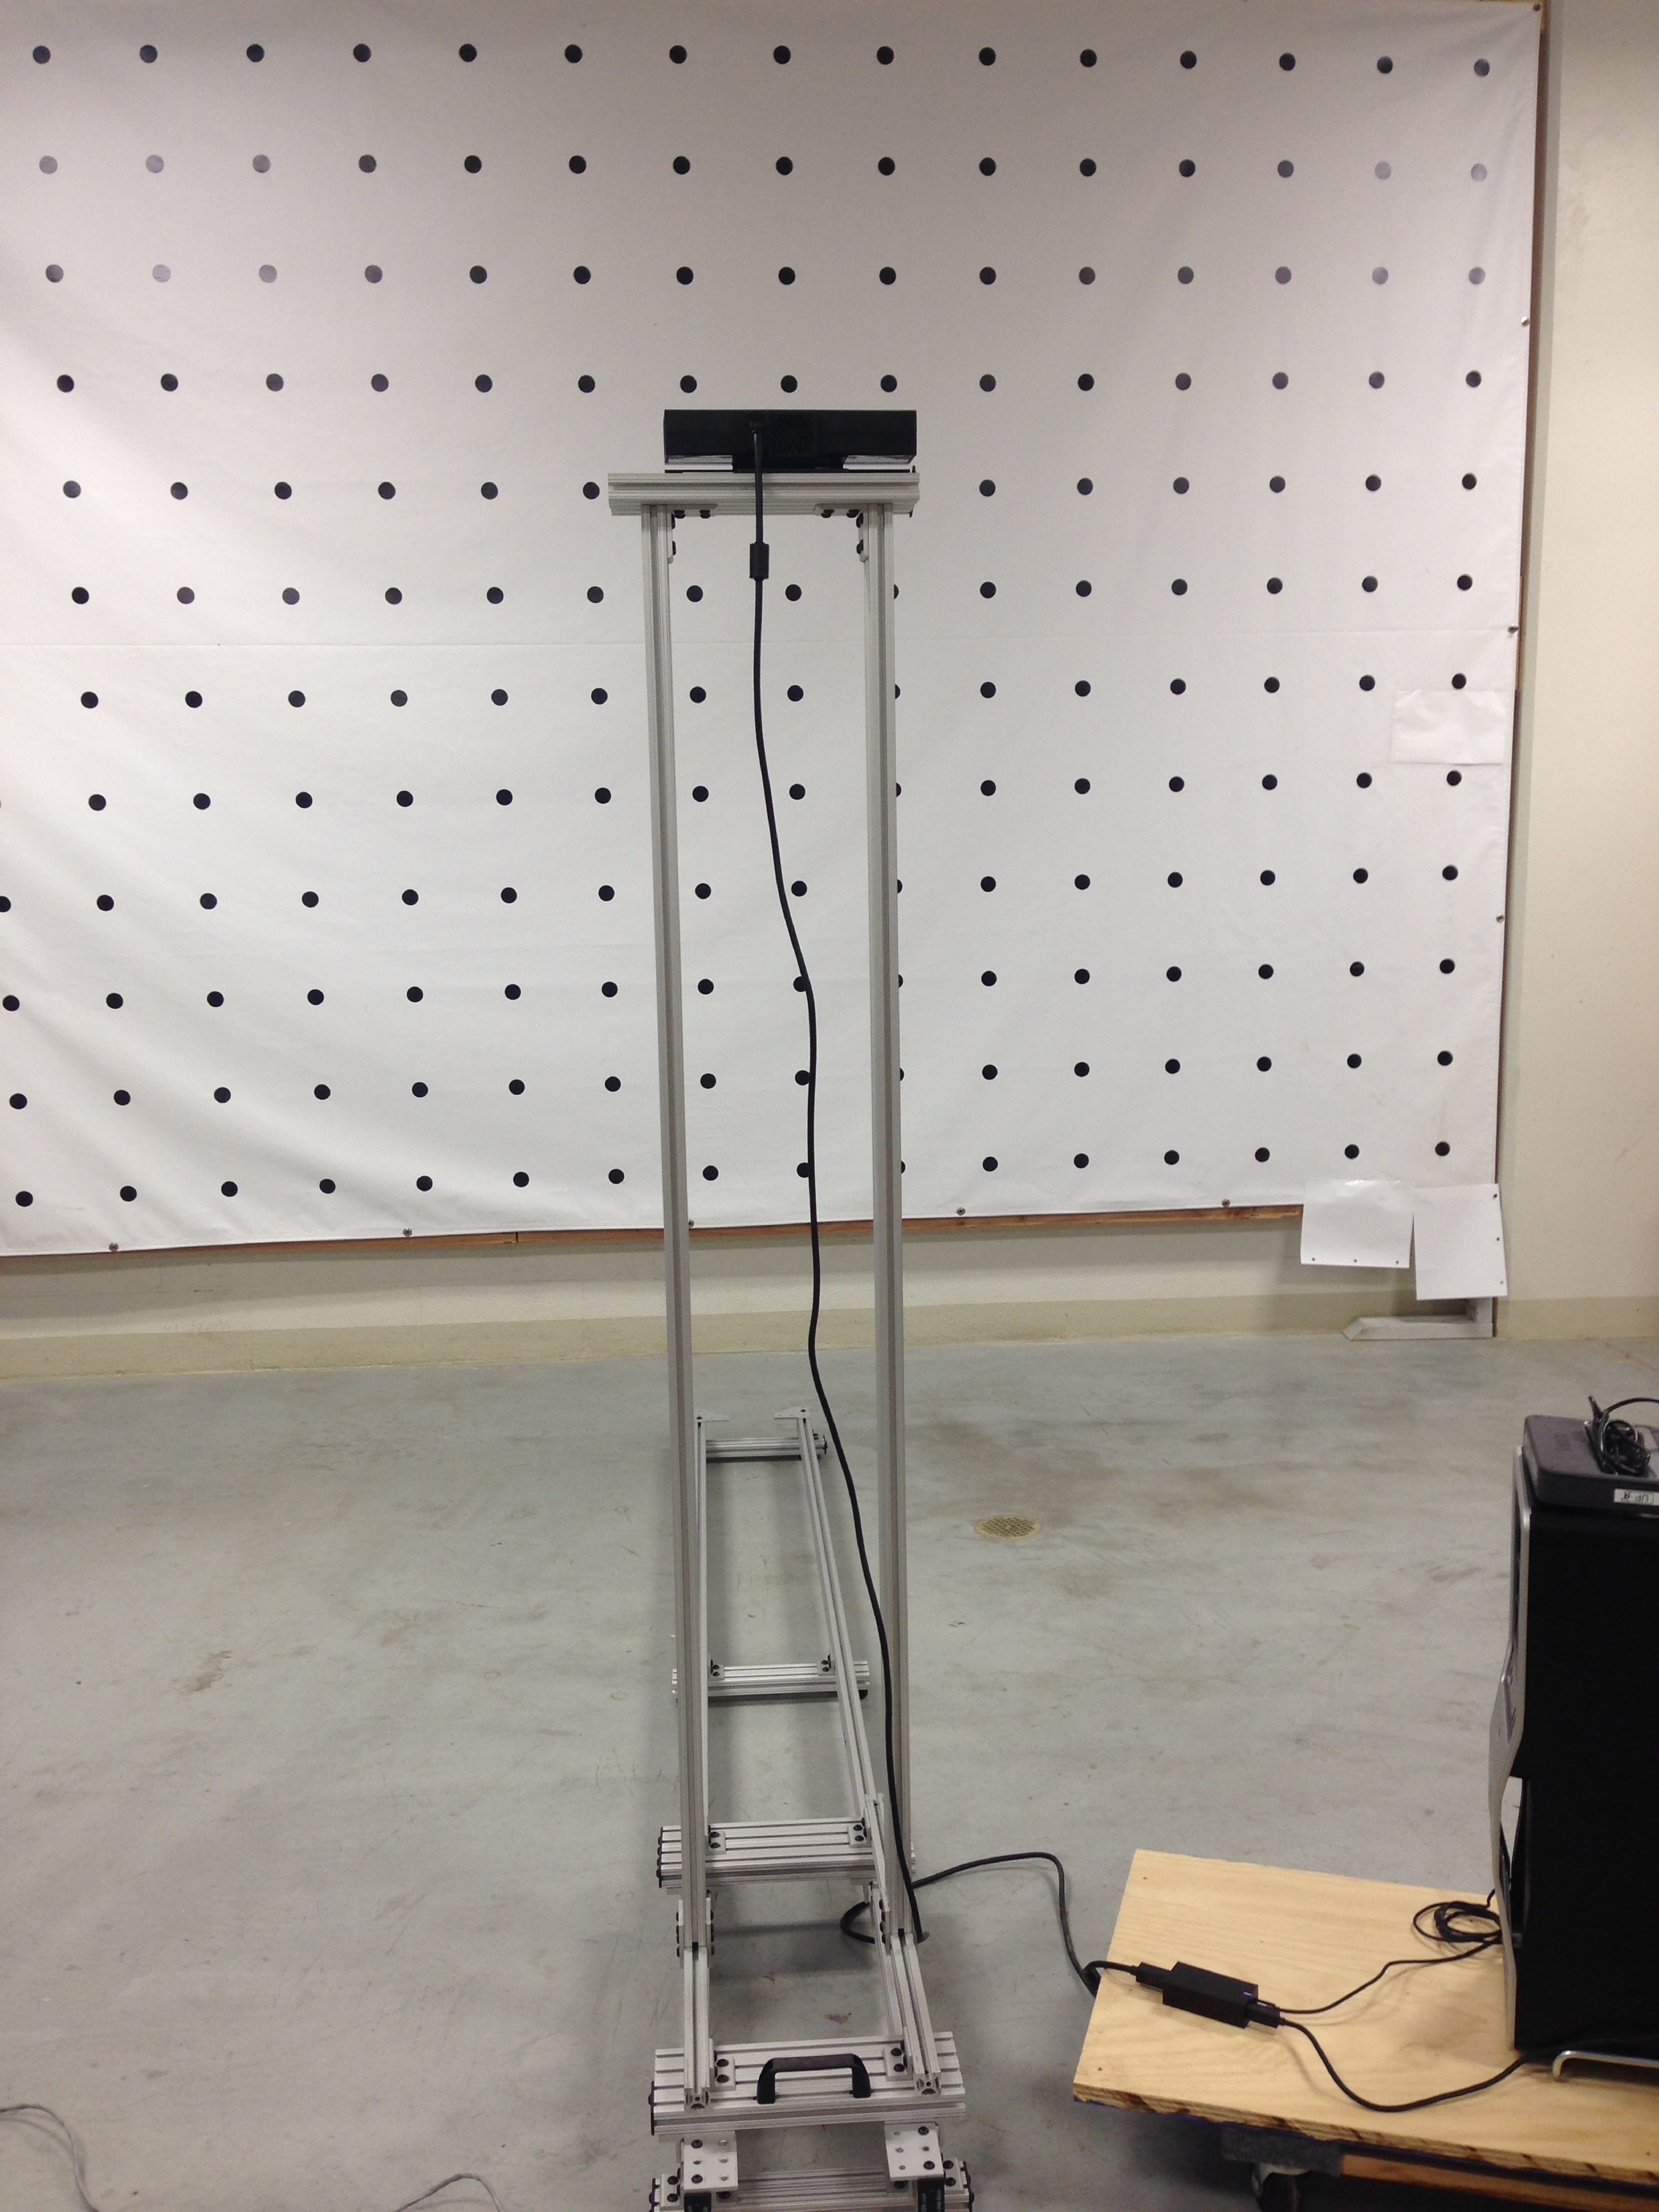
\includegraphics[width=0.5\textwidth]{trackingModuleOnKinectV2CalibrationSystem}
\caption{KinectV2 Calibration System}
\label{trackingModuleOnKinectV2CalibrationSystem}
\end{figure}%

As shown in figure \ref{trackingModuleOnKinectV2CalibrationSystem}, the RGB-D camera KinectV2 is mounted on the slider of the rail, which is perpendicular to the uniform round dot pattern as \(Z^{w}\) axis. With the round dot patten plane as the plane \(X^wY^w\) where \(Z^{w}\) being assumed as zero, the center point of each round dot maps to a fixed DD world coordinates. In Chapter 2, \(X^{w}\) and \(Y^{w}\) are rectified separately through a fourth order surface fitting translation from image plane row and column to directly solve the lens distortion problem in equation \ref{lensDistortion}, considering that the parameters in that equation with power level larger than 4 are negligible. Then, \(Z^{w}\) values are totally supported from external BLE optical-flow sensor, which accurately tracks camera movements along Z-axis. Finally, a XYZWRGB-D model based lookup table will be generated for real-time reconstruction. Whole calibration system will be introduced in detail in Chapter 3. Results will be shown in Chapter 4.





\section{Summation}














































% Chapter 2
%Chapter 2: 3D Rectification ( on PrimeSense, KinectV2, and Prosilica )all of equations
%2.1 From Depth to Z-coordinate
%2.2 From Z to X/Y
%2.3 3D Reconstructions for PrimeSense, KinectV2, and Prosilica
%Chapter 2: Camera Calibration Model(Compare pinhole camera  
%
%X= ExZ + Fx
%Y= EyZ + Fy
%with what we are doing)
\chapter{Real-Time 3D Rectification} % Main chapter title
\label{sens_Rectification} % For referencing the chapter elsewhere, use \ref{sens_Rectification} 
As analyzed in chapter \ref{sens_introduction}, traditional camera calibration based on pinhole camera model is not able to supply RGB-D cameras a satisfying real-time solution for lens and depth distortions. In this chapter, instead of using any models, a data based look-up table (LUT) method is used, which will not only suit for both of NearIR steams and RGB steams, but also for all of the universal RGB-D cameras. Rectifications of 3D world coordinates \(X^{w}\)/\(Y^{w}\)/\(Z^{w}\) will be separated into two parts. 
\\\\%
Above all, \(X^{w}\) and \(Y^{w}\) will be separately translated though two different transformation matrices that contains radial dominated lens distortions information. The transformation matrices are determined by pixels' coordinates-pairs ( image plan coordinates \(row\) / \(column\) and corresponding world coordinates \(X^{w}\)/\(Y^{w}\) ) that are extracted from captured uniform round dot grid pattern. Then, for each frame, external calibrated data from optical-flow sensor will be added as fixed \(Z^{w}\) for every pixel in the frame. After both of RGB stream and NearIR stream pixels find a match with world coordinate \(X^{w}\)/\(Y^{w}\)/\(Z^{w}\), depth data will be finally added for each pixel to generate a table of XYZWRGB-D.

\section{\(X^{w}\)/\(Y^{w}\) Rectifications}
\label{sectionXY_rectification}
The uniform round grid captured by RGB/NearIR steams contains radial dominated distortions information, which will be used for \(X^{w}\)/\(Y^{w}\) rectifications, to generate transform matrices to translate image plane rows and columns to world coordinates \(X^{w}\)/\(Y^{w}\). In order to appropriately make use of the distortions information, the core mission is to locate the coordinates-pairs of each round dot. \\\\
%
The whole process of transformation matrices generation could be separated into three steps. %
The first step is to track the \((column, row)\) of each round dot cluster's center captured by RGB/NearIR steams, and the second step is to determine the corresponding world coordinates \((X^w, \,Y^w)\) for every \((column, row)\). After the coordinates-pairs are determined for every round dot cluster's center captured by RGB/NearIR steams, the last step is to use them to train high-order polynomial surface fitting models to generate transformation matrices, which could map from \((column, row)\) to \((X^w, \,Y^w)\) for every single pixel of a frame.
%
\subsection{Round Dot Center \((column, row)\) extraction}
\label{RowColumnExtraction}
The round dot pattern consists of black dots and white background. As the simplest way to segment black dots from background, which is not 100\% white in the captured image, thresholding (binarizing) is applied as pre-processing of the uniform grid's tracking, using Digital Image Processing (DIP) technologies. After an adaptive binarizing of a frame, a \enquote{sniffer} (edge modification) will be applied for captured clusters' centers determination, i.e., the extraction of (column, row) as clusters' centers.\par
%
\subsubsection{Digital Image Processings}
In this section, DIP technologies are used for the goal of RGB/NearIR steams' binarizing. Considering that the many steps of processing will be applied on every single pixel of every frame, using GPU (parallel processing) has more advantages on handling this kind of mission than using CPU. OpenGL is selected as image processing language, and the default data type of steams saved on GPU during processing will be Single-Floating type, with a range from 0 (balck) to 1 (white). For both of RGB steam and NearIR steam, steam data need to be saved onto GPU first, during which progress gray-scale converting is also done.\\%
\\\par%
 \qquad \textbf{Converting RGB/NearIR to Gray-Scale}\\%
In order to suit for both of the RGB and the NearIR steams, the first step of binarizing is to do gray-scaling. For NearIR steam, its data contains only color gray. There is no need to consider gray-scale problem, and data will be saved on GPU as single-floating automatically. Whereas for RGB steam, a conversion from RGB to gray value is needed. Typically, there are three converting methods: lightness, average, and luminosity. The luminosity method is finally chosen as a human-friendly way for gray-scaling, because it uses a weighted average value to account for human perception, which could be written as

\begin{equation}
%
Intensity_{\text{\_gray}} =  0.21 Red\,  + \, 0.72 Green \, + \, 0.07 Blue
%\label{lensDistortion}
%
\end{equation}%
%
\\\par%
 \qquad \textbf{Histogram Equalization}\\%
As values saved on GPU, all of the pixel intensity values are within the range of [0, 1], where \enquote{0} means 100\% black and \enquote{1}  means 100\% white. In practical, NearIR steam image is always very dark, as shown in figure \ref{Raw_Single_NIR} (with their intensity values every close to zero).  In order to enhance the contrast of NearIR image for a better binarizing, rescaling is necessary. In this section, histogram equalization technique is used maximize the range of valid pixel intensity distributions. Same process is also compatible on the RGB steam.\\\\
%
 \begin{figure}[h]
\hspace*{-0.5cm}
\centering
\subfloat[Raw NearIR][Raw]{
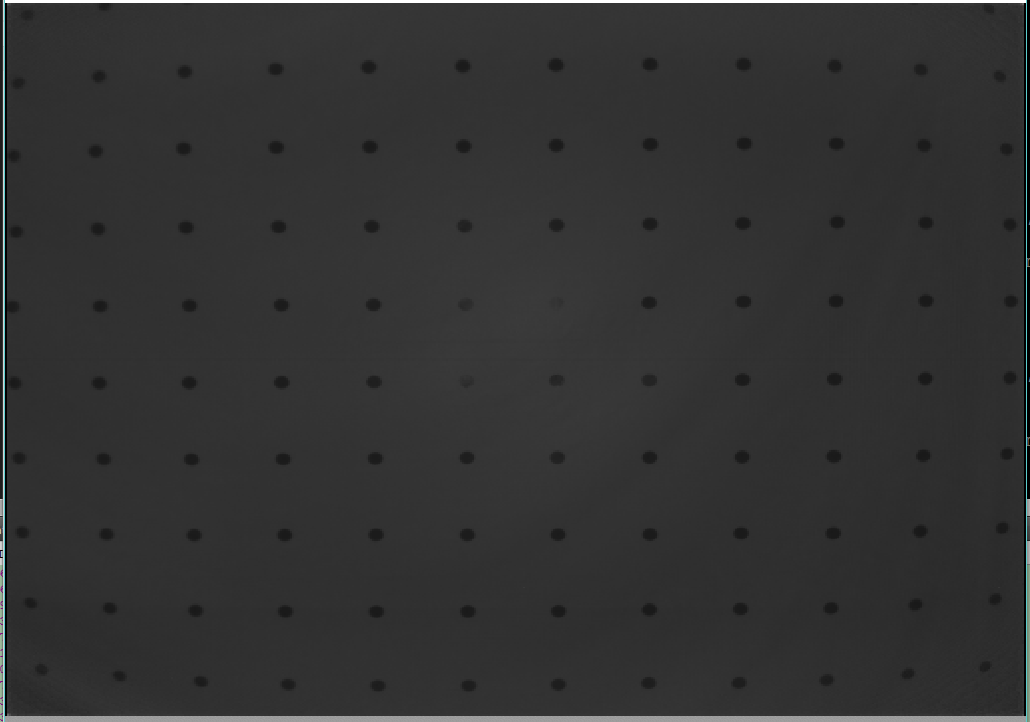
\includegraphics[width=0.5\textwidth]{Raw_Single_NIR}
\label{Raw_Single_NIR}}
\subfloat[Histogram Equalized NearIR][Histogram Equalized]{
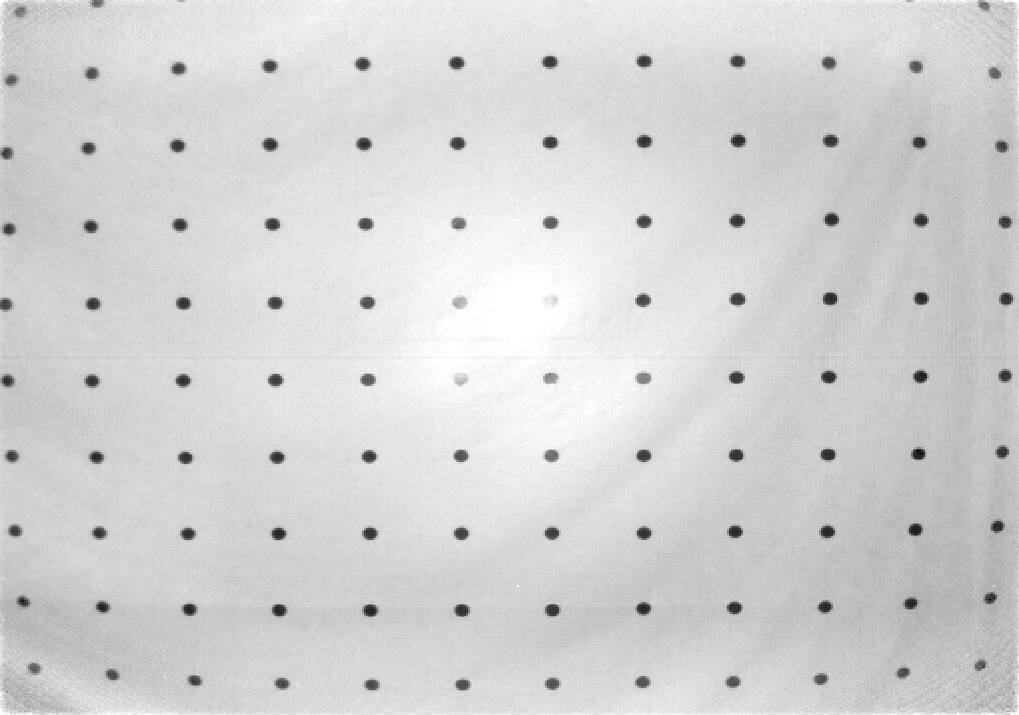
\includegraphics[width = 0.5\textwidth]{NIR_After_HistogramEqualization}
\label{NIR_After_HistogramEqualization}}
%\qquad
\caption{NearIR Streams before / after Histogram Equalization}
\label{Histogram_Equalization}
\end{figure}%
%
Commonly, Probability Mass Function (PMF) and Cumulative Distributive Function (CDF) will be calculated to determine the minimum valid intensity value (\(floor\)) and maximum valid value (\(ceiling\)) for rescaling, whereas tricks could be used by taking advantage of the GPU drawing properties.\\%
\\%
PMF means the frequency of every valid intensity value for all of the pixels in an image. Dividing all of the pixels in terms of their intensity values into \(N\) levels, every pixel belongs to one level of them, which is called gray level. With an proper selection of \(N\) to make sure a good accuracy, the intensity value of a pixel could be expressed based on its gray level \(n\), as\par%

\begin{equation}
%
Intensity = n/N * (1 - 0) + 0 = n/N
%\label{lensDistortion}
%
\end{equation}%
%
where \(n\) and \(N\) are integers and \(1 \leqslant n \leqslant N\).\\\\%
%
PMF calculation is very similar with the points-drawing process in terms of GPU that, both of them share the properties of pixel-by-pixel calculation. For the GPU points-drawing process onto a customer framebuffer, the single-floating \enquote{color} value could go beyond the normal range [0, 1], with a maximum value of a signed 32-bit integer (\(2^{31}\) - 1). And different \enquote{color} values will be added together to form a \enquote{summational-color} in the case that some pixels are drawn onto the same position coordinates. \textbf{Taking} the range of pixel intensity values [0, 1] \textbf{as} a segment on x-axis waiting to be drawn, the intensity frequency \textbf{as} the \enquote{summational-color} of multiple pixels with different intensity drawn at the same position, and the counting process of intensity frequency \textbf{as} a points-drawing process, PMF could be calculated by drawing all of the pixels onto the x-axis within the normal intensity range [0, 1], with every single pixel's position coordinates re-assigned as (\(pixel\_intensity\), \(0\)) and its \enquote{color} value constantly being equal to one. Given the width (range of x-axis) of customer framebuffer being [-1, 1] in OpenGL, which is twice the range of pixel intensity [0, 1], the half-width of the customer framebuffer is same with the total number \(N\) of gray levels, which determines the precision of \(floor\) / \(ceiling\) intensity selection. 
\\\\%
With PMF calculated and each intensity frequency that mapped to its corresponding gray level saved in the customer framebuffer, CDF could be easily calculated as
%
\begin{equation}
%
CDF(n) = \frac{sum}{N_{\text{\_Total Pixels/Image}}} 
%\label{lensDistortion}
%
\end{equation}%
%
where the gray level \(n\) is counted from the middle of the framebuffer's width to the end (1 \texttildelow \, \(N\)). And \(sum\) is the summation of customer framebuffer's values added up consecutively from 1 till \(n\).\\\\%
%
Then, at appropriate CDFs, e.g., \(CDF(n_{\text{\_floor}}) = 0.01\) and \(CDF(n_{\text{\_ceiling}}) = 0.99\), the intensities \(floor\) and \(ceiling\) could be written as
%
\begin{equation}
%
\begin{aligned}
floor &=  n_{\text{\_floor}} / N%
\\%
ceiling &=  n_{\text{\_ceiling}} / N
\end{aligned}
\label{intensityFloorCeilingDetermination}
%
\end{equation}%
%
Finally, a new intensity value of every single pixel in an image could be rescaled as
%
\begin{equation}
%
\begin{aligned}
Intensity_{\text{\_new}} &= \frac{Intensity_{\text{\_original}} - floor}{ceiling - floor} 
\end{aligned}
%
\end{equation}%
%
After this final rescaling step of Histogram Equalization, the new image gets better contrast effect, as shown in figure \ref{NIR_After_HistogramEqualization}%
\\\par%
 \qquad \textbf{Adaptive Thresholding}\\%
Affected by radial dominated lens distortions, the intensity value tend to decrease as the position of a pixel moves from the center of an image to the borders, in the case of observing a singular color view. Therefore, using fixed thresholding will generate too much noise around borders, and an adaptive thresholding process is needed. To segment the black dots from white background, we could simply subtract an image's background from an textured image. And an image's background comes from a blurring process on that image. \par%
%
 \begin{figure}[h]
\hspace*{-0.5cm}
\centering
\subfloat[Histogram Equalized NearIR][Histogram Equalized]{
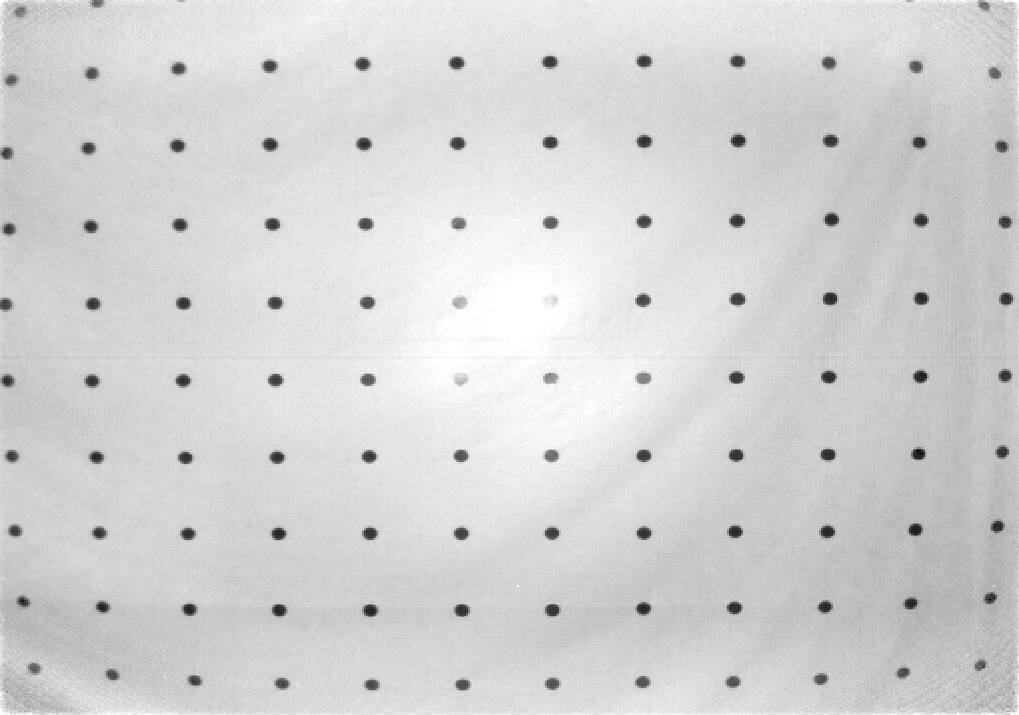
\includegraphics[width = 0.5\textwidth]{NIR_After_HistogramEqualization}
\label{NIR_After_HistogramEqualization}}
\subfloat[After Adaptive Thresholding][Binarized]{
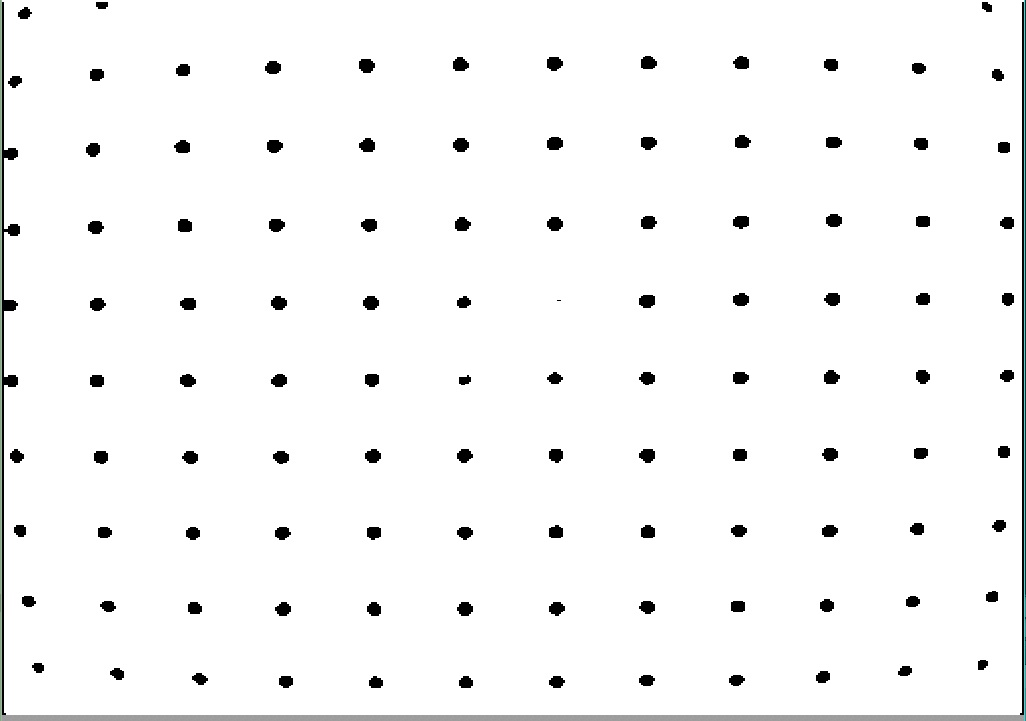
\includegraphics[width=0.5\textwidth]{Binarized_Single_NIR}
\label{Binarized_Single_NIR}}%\qquad
\caption{NearIR Streams before / after Adaptive Thresholding}
\label{Adaptive_Thresholding}
\end{figure}%
\par%
%
There are three common types of blurring filters: mean filter, weighted average filter, and gaussian filter. Mean filter is selected for this background-aimed blurring process, because it has the smallest calculation and also a better effect of averaging than the others. After the blurred image containing background information is obtained, the binarizing (subtraction) process for every single pixel could be written as

\begin{equation}
%
Intensity_{\text{\_binarized}} = %
%
\begin{cases}
\,\, 1 , \quad \quad I_{\text{\_textured}} - I_{\text{\_background}}  -  C_{\text{\_offset}} \,\, > \,\,0 %
\\%
\,\, 0 , \quad \quad \quad \quad else%
\end{cases}
%
\end{equation}%
%
where \(I\) is short for \(Intensity\) of every single pixel, and \(C_{\text{\_offset}}\) is a small constant that could be adjusted depending on various thresholding situations. In this project, \(C_{\text{\_offset}}\) is around 0.1.%
\\\\%
To sharpen the edge of the binarized image for a better \enquote{circle} shape detection, a median filter could be added as the last step of adaptive thresholding. As shown in figure \ref{Adaptive_Thresholding}, background is removed in the binarized image after adaptive thresholding.
%
%
\subsubsection{Sniffer for Round Dot Center}
After the adaptive thresholding, image data saved on GPU is now composed of circle-shaped \enquote{0}s within a background of \enquote{1}s. In order to locate the center of those \enquote{0}s circle, which is the center of captured round dot, it is necessary to know the edge of those circles. A trick is used to turn all of the edge data into markers that could lead a pathfinder to retrieve circle information.%
\\\\%
The idea that helps to mark edge data is to reassign pixels' values (intensity values) based on their surroundings. Using letter \(O\) to represent one single pixel in the center of a 3x3 pixels environment, and letters from \(A\)\texttildelow \(H\) to represent surroundings, a mask of 9 cells for pixel value reassignment could be expressed as below.

\begin{center}
  \begin{tabular}{ | c | c | c | }
    \hline
    \(E\) & \(A\) & \(F\) \\ \hline
    \(B\) & \(O\) & \(C\) \\ \hline
    \(G\) & \(D\) & \(H\) \\
    \hline
  \end{tabular}
\end{center}
%
To turn the surroundings \(A\)\texttildelow \(H\) into marks, different weights will be assigned to them. Those markers with different weights have to be non-zero data, and should be counted as the edge-part of circles. Therefore, the first step is to inverse the binary image, generating an image that consists of circle-shaped \enquote{1}s distributed in a background of \enquote{0}s.%
\\\\%
After reversing, the next step is to assign weight to the surroundings. OpenGL offers convenient automatic data type conversion, which means the intensity values from \enquote{0} to \enquote{1} of single-floating data type save on GPU could be retrieved to CPU as unsigned-byte data type from \enquote{0} to \enquote{255}. Considering a bitwise employment of markers, a binary calculation related weight assignment is used in the shader process for pixels. The intensity reassignment for every single pixel is expressed as the equation below.
%
\begin{equation}
\hspace*{-0.1cm}%
%
I_{\text{\_Path Marked}} = I_{\text{\_Original}} * \frac{(128I_{\text{A}} + 64I_{\text{B}} + 32I_{\text{C}} + 16I_{\text{D}} + 8I_{\text{E}} +  4I_{\text{F}} +  2I_{\text{G}}+I_{\text{H}})}{ 255 }
%
\label{snifferDistributionWeight}
\end{equation}%
\\%
After this reassignment, the image is not binary any more. Every non-zero intensity value contains marked information of its surroundings, data at the edge of circles are now turned into fractions. In other words, the image data saved on GPU at the moment is composed of \enquote{0}s as background and \enquote{non-zero}s circles, which contains fractions at the edge and \enquote{1}s in the center.%
\\\\%
Now, it is time to discover dots through an inspection over the whole path-marked image, row by row and pixel by pixel. Considering that, a process of one single pixel in this step may affect the processes of the other pixels (which cannot be a parallel processing), it is necessary to do it on CPU. The single-floating image data will be retrieved from GPU to a buffer on CPU as unsigned-byte data, waiting for inspection. And correspondingly the new CPU image will have its \enquote{non-zero}s circles composed of fractions at the edge and \enquote{1}s in the center. Whenever a non-zero value is traced, a dot-circle is discovered and a singular-dot analysis could start. The first non-zero pixel will be called as an anchor, which means the beginning of a singular-dot analysis. %
\\\\%
During the singular-dot analysis beginning from the anchor, very connected valid (non-zero) pixel will be a stop, and a \enquote{stops-address} queue buffer is used to save addresses of both visited pixels and the following pixels waiting to be visited. On very visit of a pixel, there is a checking procedure to find out valid (non-zero) or not. Once valid, the following two steps are waiting to go. The first step is to sniff, looking for possible non-zero pixels around as the following stops. And the second step is to colonize this pixel, concretely, changing the non-zero intensity value to zero. Every non-zero pixel might be checked 1\texttildelow 4 times, but will be used to sniff for only once.%
\\\\%
As for the sniffing step, base on the distribution table of \(A\)\texttildelow \(H\) that has been discussed above and their corresponding weight given by equation \ref{snifferDistributionWeight}, the markers \(A\)/\(B\)/\(C\)/\(D\) are valid (non-zero) as long as the intensity value of pixel \(O\) satisfies the following conditions shown as below.%
%
\begin{equation}
%
\begin{aligned}
if \,\, ( I_{\text{O}} \,\, \& \,\, \text{0x80}  == 1 ),\quad &then, \quad \text{marker } A\,\, \text{is valid \,\,( go Up )}%
\\%
if \,\, ( I_{\text{O}} \,\, \& \,\, \text{0x40}  == 1 ),\quad &then, \quad \text{marker } B\,\, \text{is valid \,\,( go  Left)}%
\\%
if \,\, ( I_{\text{O}} \,\, \& \,\, \text{0x20}  == 1 ),\quad &then, \quad \text{marker } C\,\,\text{is valid \,\,( go Right )}%
\\%
if \,\, ( I_{\text{O}} \,\, \& \,\, \text{0x10}  == 1 ),\quad &then,\quad \text{marker } D\,\,\text{is valid \,\,( go Down )}%
\\%
\end{aligned}
%
\end{equation}%
%
Once a valid marker is found, its address \((column, row)\) will be saved into the \enquote{stops-address} queue. One pixel's address might be saved for up to 4 times, but \enquote{colonizing} procedure will only happen once at the first time, so that the sniffing will stop once all of the connected valid pixels in a singular dot-cluster are colonized as zeros.%
\par%
%
 \begin{figure}[h]
\hspace*{-0.5cm}
\centering
\subfloat[After Adaptive Thresholding][before Extraction]{
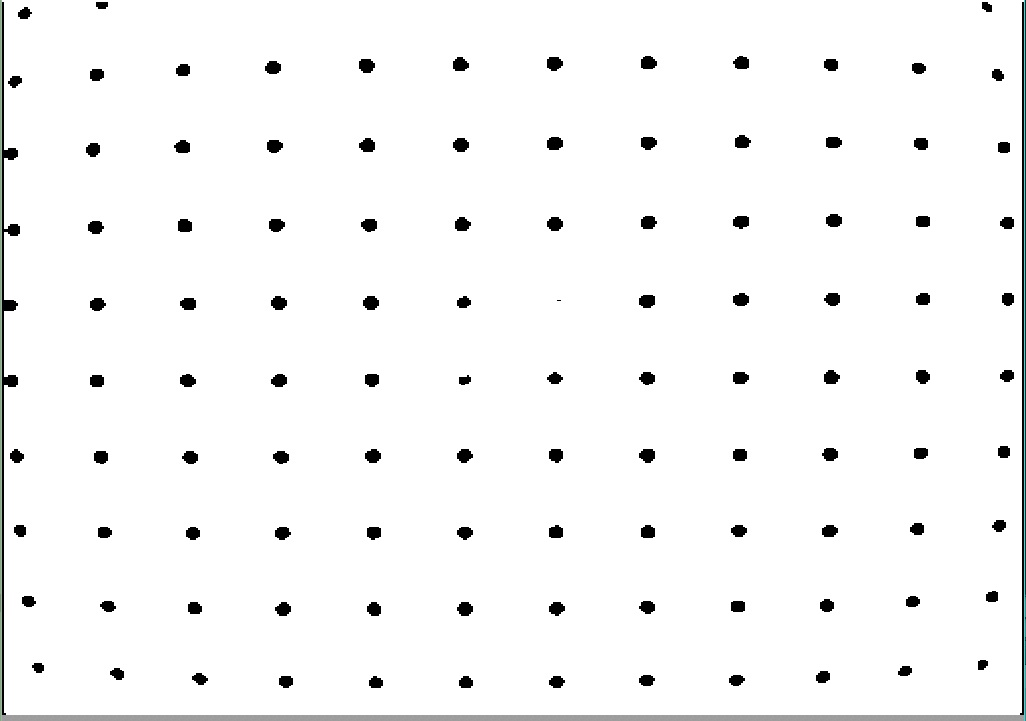
\includegraphics[width=0.5\textwidth]{Binarized_Single_NIR}
\label{Binarized_Single_NIR}}
%\qquad
\subfloat[Dot Centers Extraction][Extracted and Marked]{
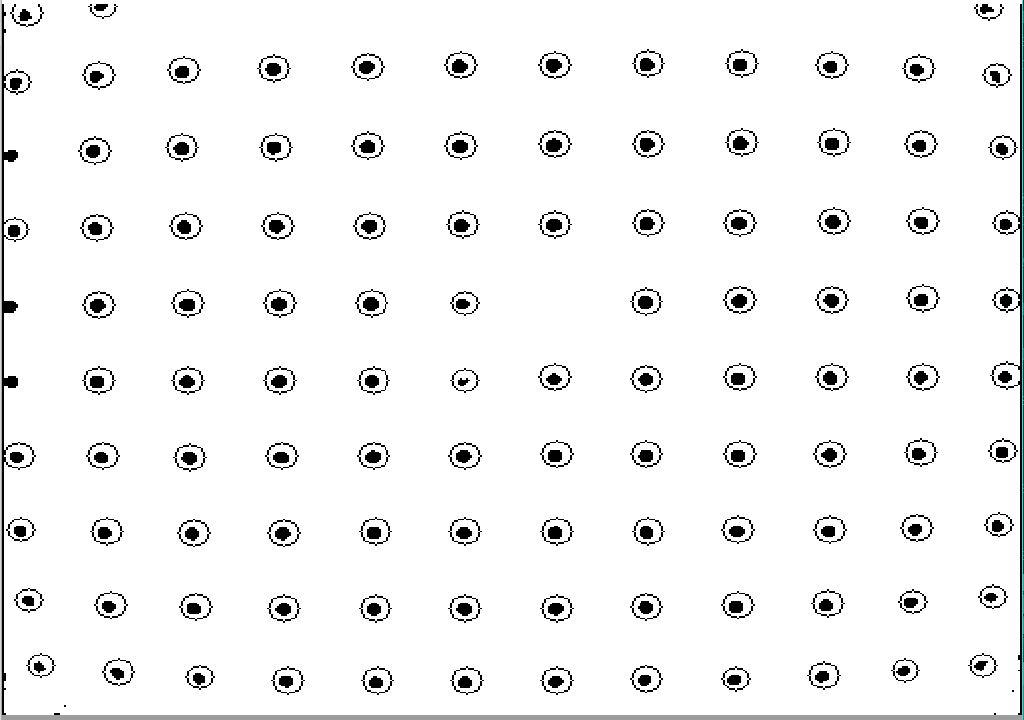
\includegraphics[width = 0.5\textwidth]{Dots_Extracted_Single_NIR}
\label{Dots_Extracted_Single_NIR}}
%
\caption{Valid Dot-Clusters Extracted in NearIR}
\label{DotCentersExtraction}
\end{figure}
%
In the second step \enquote{colonizing},  \(I_{\text{O}}\) is changed to zero, variable \(area\) of this dot-cluster pluses one, and bounding data \(RowMax\) / \(RoxMin\) / \(ColumnMax\) / \(ColumnMin\) are also updated.%
\\\\%%
Finally, the Round Dot Centers \((column, row)\) could be determined as the center of bounding boxes with their borders \(RowMax\) / \(RoxMin\) / \(ColumnMax\) / \(ColumnMin\). After potential noises being removed based on their corresponding \(area\) and shape (ratio of width and height), the data left are taken as valid dot-clusters. As shown in figure \ref{Dots_Extracted_Single_NIR}, the centers of valid dot-clusters are marked within their corresponding homocentric circles.
%
%
\subsection{\((X^w, \,Y^w)\) Fitting based on Uniform Grid}
\label{uniformGridFittingXY}
%
The list of round dot centers \((column, row)\)s is extracted through section \ref{RowColumnExtraction}. The following is to map every dot center's \((column, row)\) to its corresponding world coordinates \((X^w, \,Y^w)\). As shown in figure \ref{trackingModuleOnKinectV2CalibrationSystem}, world coordinates are from the uniform grid. Taking the side of unit-square (distance between two adjacent dots) as \enquote{Unit One} in the world coordinates and one dot as the origin of plan \(X^wY^w\), every dot cluster's center \(column\) / \(row\) will be mapped to integer values \(X^w\)/\(Y^w\). %
\\\\%
Ideally, a 3x3 perspective transformation matrix could help set a linear mapping between two plane coordinates, and 3 dot centers with know coordinates pair of \((column, row)\) and \((X^w, \,Y^w)\) are enough to determine the transformation matrix. Once four points with a squared-shape \(column\)/\(row\) distribution is found, a 3x3 perspective transformation matrix \(A\) could be determined by solving%
%
\begin{equation}
%
\left[ \begin{array}{c} %
zX^w \\ zY^w \\ z \end{array} \right] %
= %
A\cdot \left[ \begin{array}{c} %
C \\ R \\ 1 \end{array} \right] %
= %
\begin{bmatrix} 
a_{11} & a_{12} & a_{13} \\
a_{21} & a_{22} & a_{23} \\
a_{31} & a_{32} & a_{33} \\
\end{bmatrix}%
\cdot \left[ \begin{array}{c} %
C \\ R \\ 1 \end{array} \right] %
%
\label{perspectiveDistortionCorrectionEquation}
\end{equation}%
%
where \(C\) and \(R\) are vectors consist of \((column, row)\)s of four squared-shape distributed points; \(X^w\) and \(Y^w\) are vectors consist of four points \((0, 0)\), \((0, 1)\), \((1, 1)\), and \((1, 0)\); \(z\) denotes the third axis in the homogenous system connecting two planes. %
\\\\%
Due to the distortions, cluster centers in image plane are not uniformly distributed, and this 3x3 transformation matrix can only generate corresponding decimal \(X^w\)/\(Y^w\) values that are close integers. But in practical, the correct integer values \(X^w\)/\(Y^w\) could still be calculated through \(Rounding\). The list of cluster centers' image coordinate \((column, row)\)s can give many groups of four squared-shape distributed points, while each of them gives a different image coordinate distance that maps to the \enquote{Unit One} in world coordinates. Taking those points with generated \(X^w\)/\(Y^w\) values that are within an appropriate range close to integers as valid points, the \enquote{best} 3x3 transformation matrix could be determined by going through all of the possible groups of four squared-shape distributed points and picking out the group that leads to the most valid points.%
\\\\%
In this way, the so-called \enquote{best} transformation matrix can give a best \enquote{Unit One} distance in image coordinate, however its corresponding origin point \((0, 0)\), one of the four points that are used to calculate a transformation matrix, is usually not close to the center of cameras' Field of View (FoV). A translation matrix \(T\) could be used to refine the \enquote{best} transformation matrix, and help to translate the origin point to be a dot cluster that is closest to the center of FoV. The refined transformation matrix \(A_{\text{\_refined}}\) is written as%
%
\begin{equation}
%
A_{\text{\_refined}}%
= %
T \cdot A %
= %
\begin{bmatrix} 
1 & 0 & -X_{\text{\_Zero\_A}} \\%
0 & 1 & -Y_{\text{\_Zero\_A}} \\%
0 & 0 &   1 \\%
\end{bmatrix}%
\cdot A%
%
\end{equation}%
%
where the integer world coordinate point \((X_{\text{\_Zero\_A}}, \, Y_{\text{\_Zero\_A}})\) are mapped from the center point \((C_{\text{\_center}}, \, R_{\text{\_center}})\) of FoV in image plane by the so-called \enquote{best} transformation matrix \(A\), written as%
%
\begin{equation}
%
\left[ \begin{array}{c} %
zX_{\text{\_Zero\_A}} \\ zY_{\text{\_Zero\_A}} \\ z \end{array} \right] %
= %
A\cdot \left[ \begin{array}{c} %
C_{\text{\_center}} \\ R_{\text{\_center}} \\ 1 \end{array} \right] %
%
\end{equation}%
%
Eventually, the refined transformation matrix eventually generates a list of world coordinate points \((X^w, \, Y^w)\)s that correspond to image coordinates \((column, row)\)s. As shown in figure \ref{XY_GridFitting_Matlab}, world coordinates are integers and the origin (blue circle) is chosen as where the center-closest dot-cluster is sitting.\par%
%
 \begin{figure}[h]
\hspace*{-0.3cm}
\centering
\subfloat[Image Plane Coordinates][ImagePlane Coordinate]{
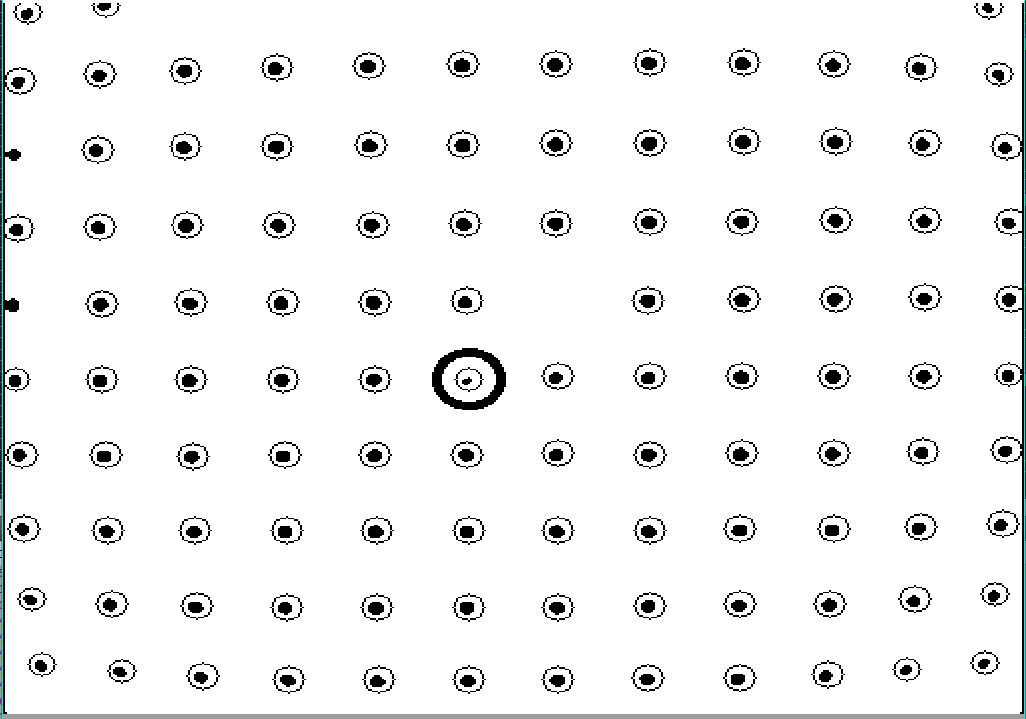
\includegraphics[width=0.54\textwidth, height = 0.425\textwidth]{Grid_Centered_Single_NIR}
\label{Grid_Centered_Single_NIR}}
%\qquad
\subfloat[World Coordinates][World Coordinate]{
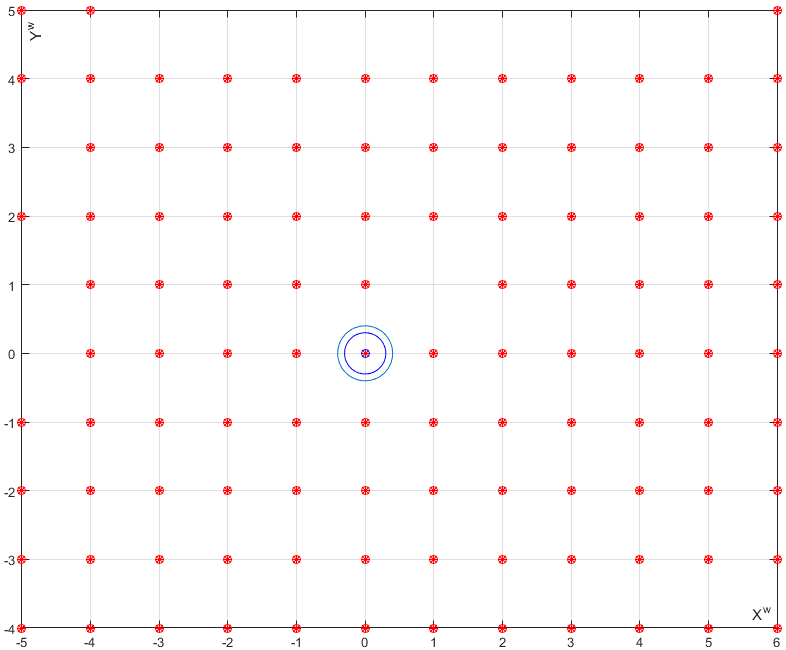
\includegraphics[width = 0.47\textwidth, height = 0.425\textwidth]{XY_GridFitting_Matlab}
\label{XY_GridFitting_Matlab}}
%
\caption{Coordinates-Pairs: (Row, Column)s and (\(X^w\), \(Y^w\))s}
\label{Grid_Fitting}
\end{figure}%
%
%
\subsection{High Order Polynomial Surface Mapping}
\label{sectionHighOrderPolynomialSurfaceMapping}
%
Using four squared-shape distributed dots, the 3x3 transformation matrix can help to find the integer value list of  world coordinate \(X^w\)/\(Y^w\). Further with all extracted dots' coordinate-pairs, a perspective distortion correction (\(1^{st}\) order polynomial with \(z\) bound) could be applied using equation \ref{perspectiveDistortionCorrectionEquation}. As shown in figure \ref{Perspective_QtScreenShot}, the \(1^{st}\) order polynomial correction is not able to handle non-linear distorted mapping. Based on the lens distortion equation \ref{lensDistortion}, a higher order two-dimensional polynomial transformation matrix is needed for both of \(x\) and \(y\) rectification. Considering that the parameters in that equation, which means a surface mapping polynomial function, with power level larger than four are practically negligible, both of the second order and fourth order polynomial mapping are discussed below (prototyped in Matlab and realized in real-time image plane rectification).\\\\%
%
The second order polynomial mapping has 2x6=12 parameters, written as %
%
\begin{equation}
%
\begin{aligned}
X^w &=  a_{11}C^2 + a_{12}CR + a_{13}R^2 + a_{14}C + a_{15}R + a_{16}
\\%
Y^w &=  a_{21}C^2 + a_{22}CR + a_{23}R^2 + a_{24}C + a_{25}R + a_{26}
\end{aligned}
\label{secondOrderPolynomial}
%
\end{equation}%
%
similarly, the fourth order polynomial mapping has 2x15=30 parameters,\par%
%
\begin{equation}
%
\hspace*{-0.3cm}%
\begin{aligned}
X^w &=  a_{11}C^4 + a_{12}C^3R + a_{13}C^2R^2 + a_{14}CR^3 + a_{15}R^4 + a_{16}C^3 + a_{17}C^2R \\%
&\,\,\,\,\,\,+ a_{18}CR^2 + a_{19}R^3 + a_{110}C^2 + a_{111}CR + a_{112}R^2 + a_{113}C + a_{114}R + a_{115}
\\\\%
Y^w &=  a_{21}C^4 + a_{22}C^3R + a_{23}C^2R^2 + a_{24}CR^3 + a_{25}R^4 + a_{26}C^3 + a_{27}C^2R \\%
&\,\,\,\,\,\,+ a_{28}CR^2 + a_{29}R^3 + a_{210}C^2 + a_{211}CR + a_{212}R^2 + a_{213}C + a_{214}R + a_{215}
\end{aligned}
\label{fourthOrderPolynomial}
%
\end{equation}%
\\\par%
%
where \(C\) and \(R\) are shorted for \(Column\) and \(Row\).
\\\\%
To prototype equation \ref{secondOrderPolynomial} and \ref{fourthOrderPolynomial} in Matlab, \enquote{Curve Fitting Toolbox} is used to obtain the 2x6 and 2x15 parameters. Once those two set of parameters are obtained, the rectified image could also be determined, as shown in figure \ref{MatlabPrototpyeOfHighOrder},\par%
%
\begin{figure}[h]
\hspace*{-0.3cm}
\centering
\subfloat[\(2^{nd}\) Order][\(2^{nd}\) Order]{
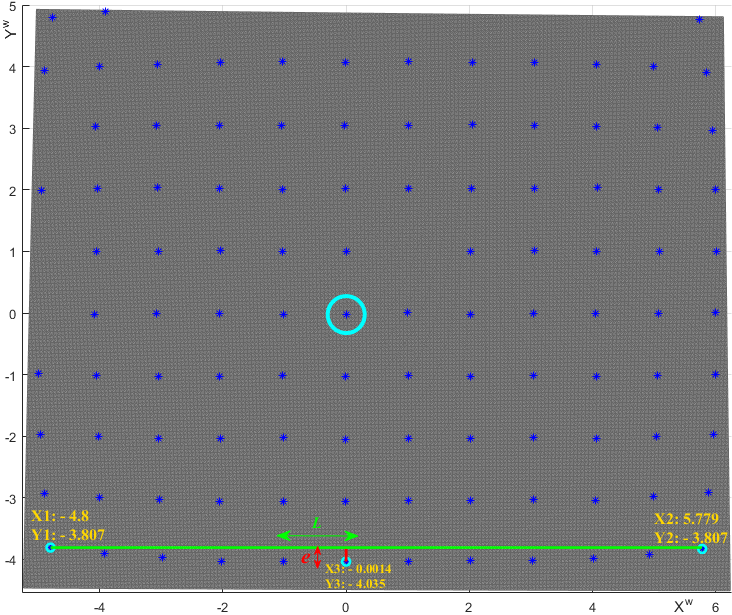
\includegraphics[width=0.5\textwidth]{Second_MatlabPrototype}
\label{Second_MatlabPrototype}}
%\qquad
\subfloat[\(4^{th}\) Order][\(4^{th}\) Order]{
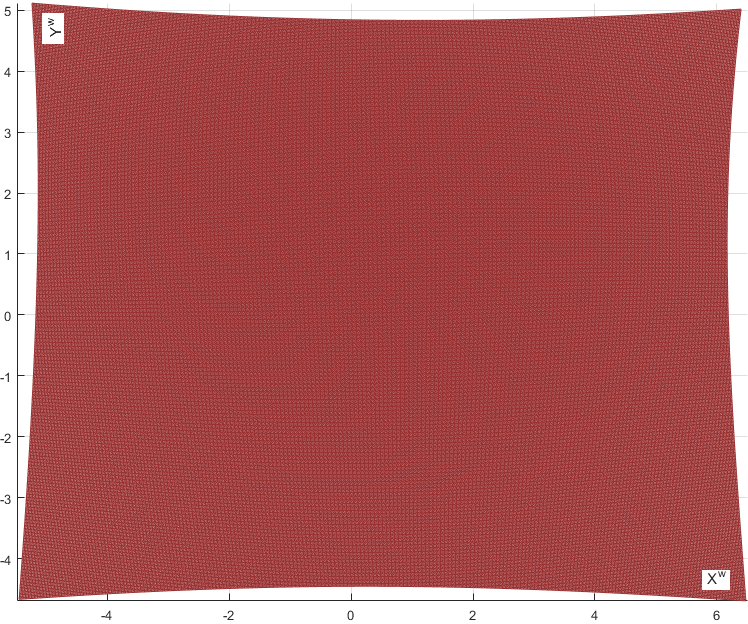
\includegraphics[width = 0.5\textwidth]{Fourth_MatlabPrototype}
\label{Fourth_MatlabPrototype}}
%
\caption{\(X^w\)/\(Y^w\) Matlab Prototype, \(2^{nd}\) / \(4^{th}\) Order Polynomial}
\label{MatlabPrototpyeOfHighOrder}
\end{figure}%
%
where based on \enquote{Goodness of fit} from Matlab, the Root-Mean-Square Error (RMSE) of (\(X^w\), \(Y^w\)) is (0.06796, 0.05638) for the \(2^{nd}\) order polynomial, and (0.02854, 0.02343) for the \(4^{th}\) order polynomial.
\\\\%
%
 \begin{figure}[h]
\centering
\hspace*{-0.3cm}
\subfloat[Before Rectification][Before Rectification]{
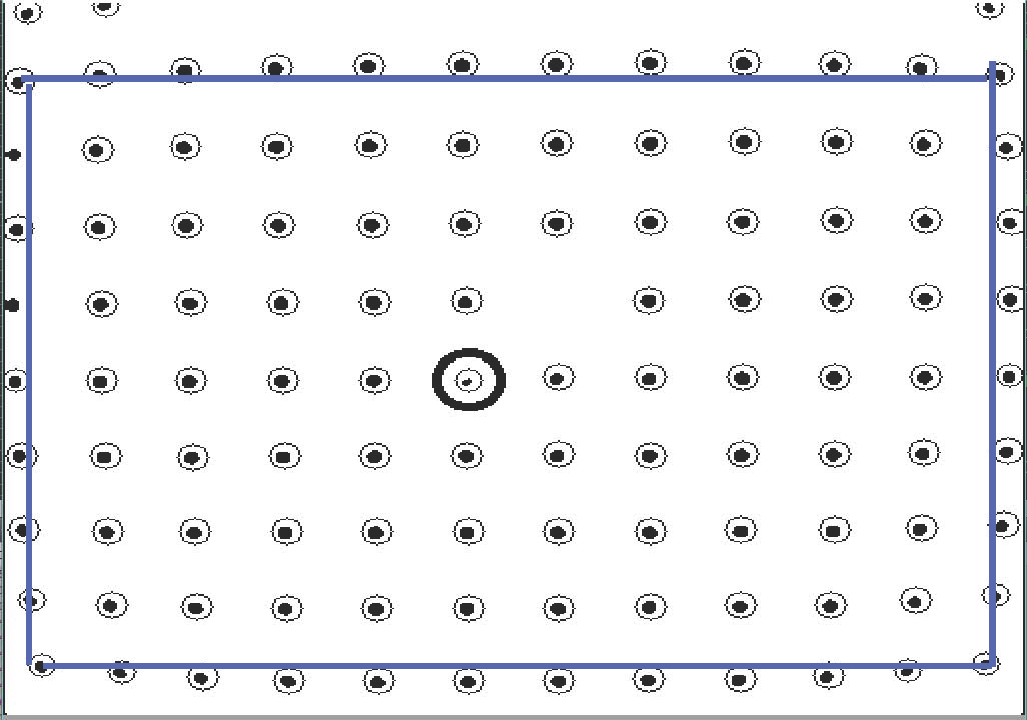
\includegraphics[width=0.5\textwidth, height = 0.425\textwidth]{BeforeRectification_Single_NIR}
\label{BeforeRectification_Single_NIR}}
%
\subfloat[Perspective Correction][Perspective (\(1^{st}\))]{
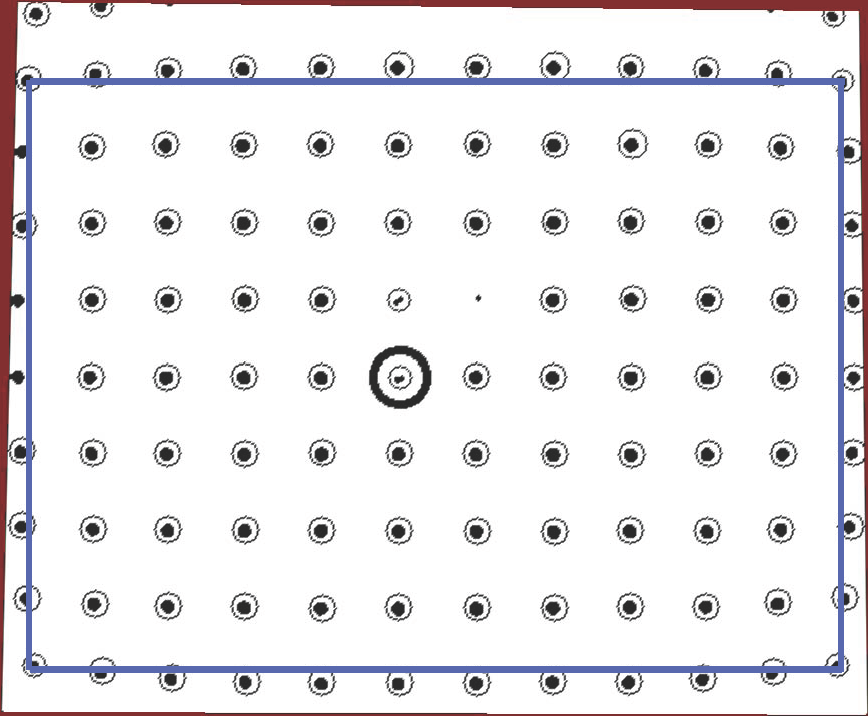
\includegraphics[width = 0.5\textwidth, height = 0.425\textwidth]{Perspective_QtScreenShot}
\label{Perspective_QtScreenShot}}
%
\\%\qquad
\hspace*{-0.3cm}
\subfloat[\(2^{nd}\) Order][\(2^{nd}\) Order]{
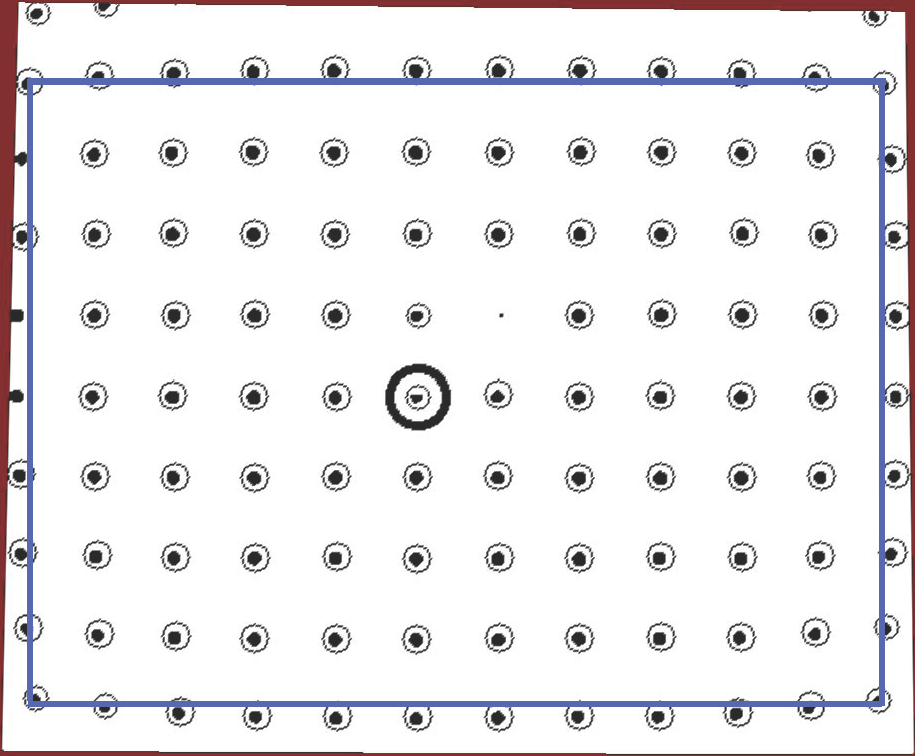
\includegraphics[width = 0.5\textwidth, height = 0.425\textwidth]{Second_QtScreenShot}
\label{Second_QtScreenShot}}
%
\subfloat[\(4^{th}\) Order][\(4^{th}\) Order]{
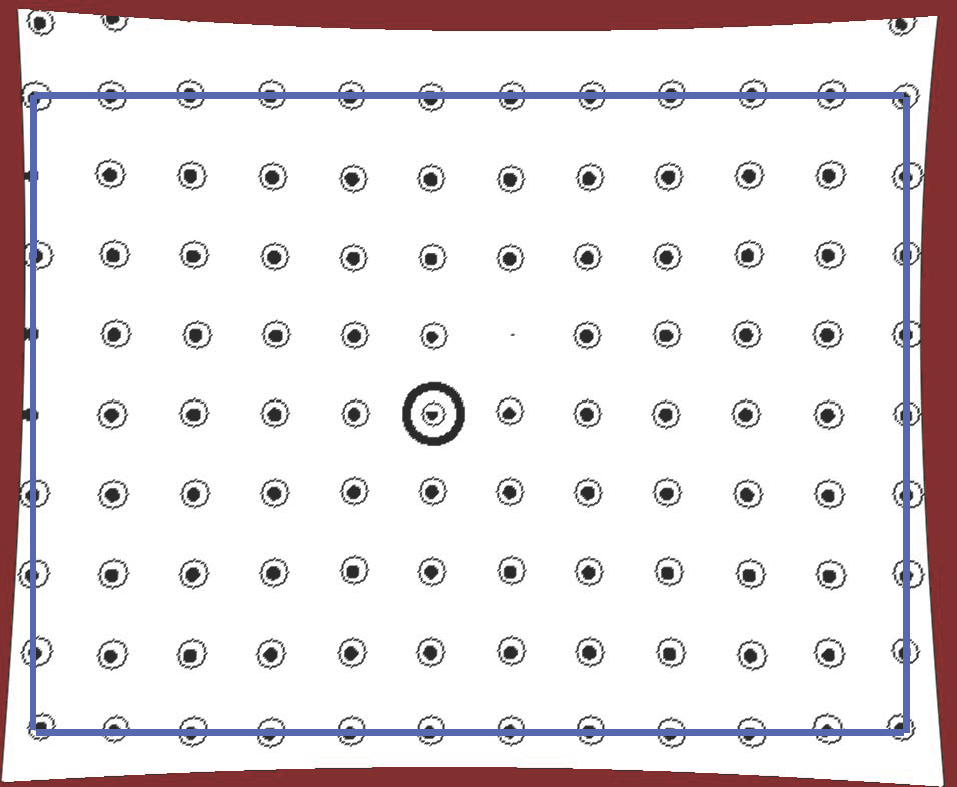
\includegraphics[width = 0.5\textwidth, height = 0.425\textwidth]{Fourth_QtScreenShot}
\label{Fourth_QtScreenShot}}
%
\caption{NearIR Stream High Order Polynomial Rectification}
\label{HighOrderNearIRRectification}
\end{figure}%
%
Then, apply those polynomial surface mappings into real-time steams rectification. We can see the rectified steam image (figure \ref{Second_QtScreenShot} and figure \ref{Fourth_QtScreenShot}), whose image-outline are same with Matlab prototypes (figure \ref{Second_MatlabPrototype} and figure \ref{Fourth_MatlabPrototype}). Comparing among the four results shown in figure \ref{HighOrderNearIRRectification}, the more dot-clusters sitting on the blue rectangle, the less distortion an image has.%
\\\\%
Not only from the comparison of RMSE, but more intuitively from figure \ref{HighOrderNearIRRectification}, we can tell that the \(4^{th}\) order polynomial surface mapping is much better than the second order (which is similar to the perspective correction). However, that more accurate process also cost more calculations, and requires more data (coordinate-pairs) to train the transformation model. Limited by the static dot pattern, fewer and fewer dot-clusters could be observed by the camera as the camera getting closer to the dot pattern. Practically, \(4^{th}\) order rectification is replaced by \(2^{nd}\) order when the number of dot-clusters is too few to train its transformation model.
%
%\subsection{Mathematical tools}
%\subsubsection{Singular Value Decomposition (SVD)}
%\subsubsection{Least Square with Pseudo-Inverse}
%
%
\section{\(Z^{w}\) Rectification}
%
Instead of from Depth steam, \(Z^{w}\) values will be determined directly from external real-world data. With the help of BLE Optical-Flow tracking module, as will be discussed later in section \ref{BLE_OF_TrackingModule}, \(Z^{w}\) values will be supported for every frame in real-time based on the camera's distance to the pattern. All of the pixels in one frame share the same \(Z^{w}\) in world coordinate.%
\\\\%
As well as the determination of \(X^{w}\)/\(Y^{w}\), which has been discussed in section \ref{uniformGridFittingXY},  \(Z^{w}\) value is also based on the uniform-grid's \enquote{Unit One},  the side of unit-square of the grid pattern. Concretely, the distance between every two adjacent dots' centers in real-world is 228mm. Therefore, \(Z^{w}\) = -\(|Z|\)(mm)/ 228(mm), where \(Z\) is the camera's working distance from the camera to dots pattern in reality offered by the BEL Optical-Flow tracking module. Choosing the origin to be where the camera is sitting, and the positives of \(X^{w}\)\(Y^{w}\) to be right and up, the \(Z^{w}\) values are always negative. Figure \ref{OneFrameXYZ_Rectified} shows one frame of 3D reconstruction in world coordinates based on rectified \(X^{w}\)/\(Y^{w}\) and \(Z^{w}\), where both of the origin and \(Z\)-axis are high-lighted as blue.%
%
\begin{figure}[h]
\centering
%rectified \(X^{w}\)/\(Y^{w}\) and \(Z^{w}\)
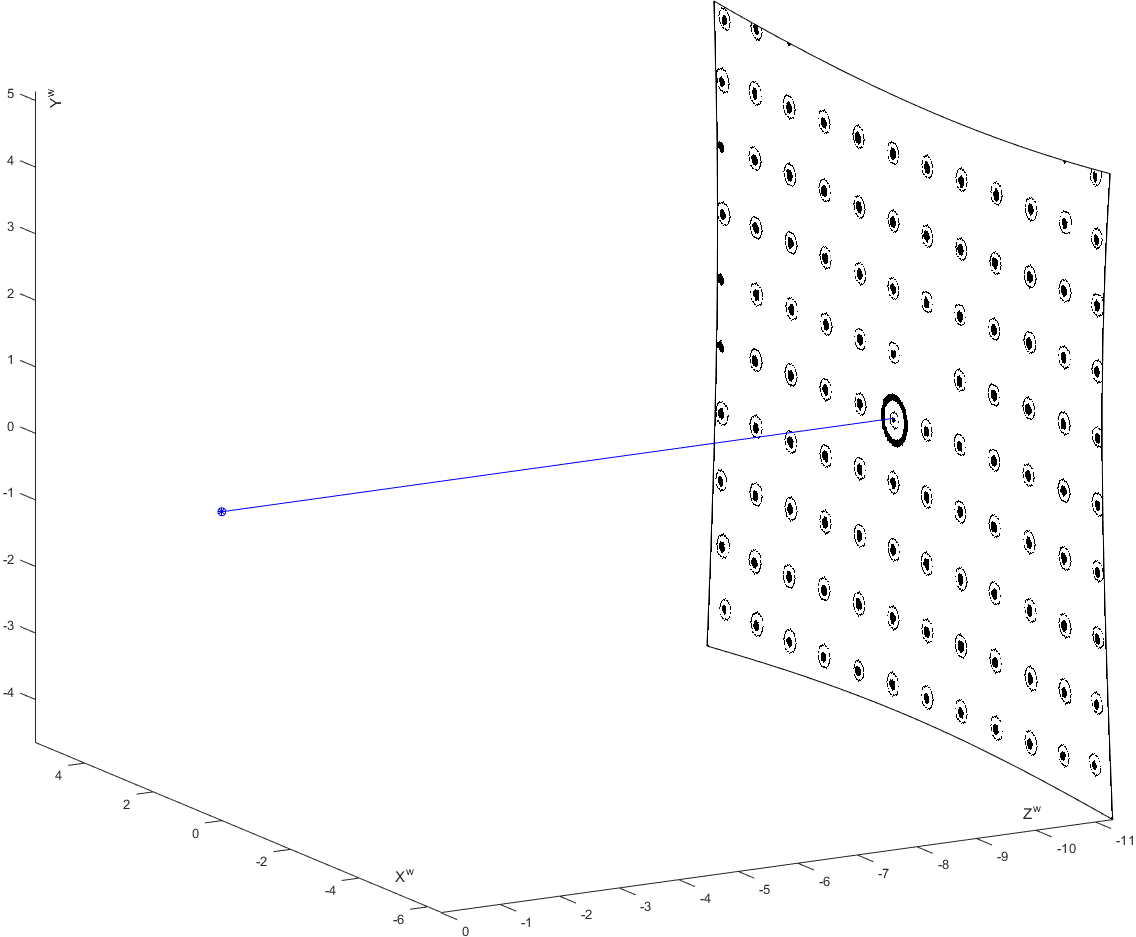
\includegraphics[width=0.7\textwidth, height= 0.5\textwidth]{OneFrameXYZ_Rectified}
\caption{NearIR Rectified \(X^{w}\)/\(Y^{w}\)/\(Z^{w}\) 3D Re-construction}
\label{OneFrameXYZ_Rectified}
\end{figure}%
%
\section{Data-Based XYZWRGB-D Look-Up Table}
In 3D re-construction, \(R\)/\(G\)/\(B\) and \(D\) (short for \(Depth\)) values are given for every pixel in one frame, while the rectified \(X\)/\(Y\)/\(Z\) (short for \(X^{w}\)/\(Y^{w}\)/\(Z^{w}\) in this section) values are determined by processes of looking up and calculating, which is based on \(D\). Therefore, the mission in this section is to find mappings from \(D\) to \(X\)/\(Y\)/\(Z\). Considering that, both of \(D\) and \(Z\) denote the distance from the camera to the object (dots pattern), it is straight forward to start from the relationship between \(D\) and \(Z\). As long as \(Z\) is obtained, \(X\) and \(Y\) for one single pixel could be determined through a linear relationship, due to the fact that the ray propagation is along a straight line.\\%
%
\begin{figure}[h]
\centering
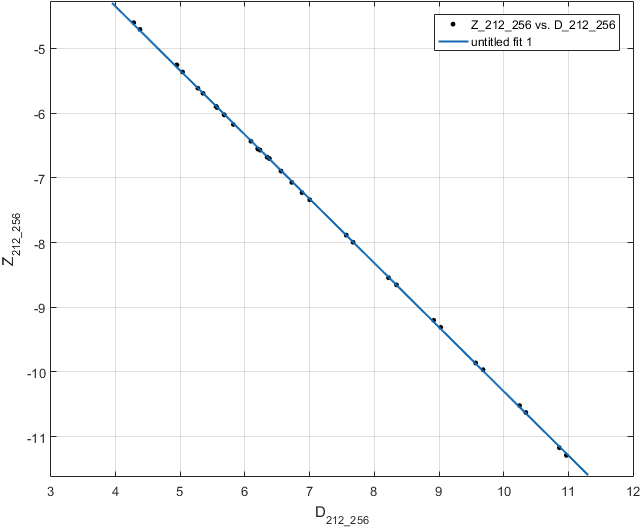
\includegraphics[width=0.8\textwidth]{ZD_CurveFitting}
\caption{Polynomial Fitting between D and Z}
\label{ZD_CurveFitting}
\end{figure}%
%
%%
%
\subsection{From \(D\) to \(Z\)}
%%
Both of \(D\) and \(Z\) are continuous data, so that their function could written as a polynomial expression, based on Taylor series. Figure \ref{ZD_CurveFitting} shows the polynomial fitting result, with 32 \(D\)/\(Z\) values (at pixel \(column\)=256 and \(row\)=212) from 32 frames, from Matlab \enquote{Curve Fitting Tool} toolbox. It is apparent that \(Z\) is linear with \(D\), which is also reasonable. Therefore, for every single pixel, \(Z\) could be retrieved from \(D\) through \par
%
\begin{equation}
Z(col, \, row) = a_{(col, row)}D(col, \, row)+b_{(col, row)}
\label{fromD_To_Z}
\end{equation}%
%
where \({(col, row)}\) denote the address of a pixels,  \(a_{(col, row)}\) and \(b_{(col, row)}\) are the corresponding linear coefficients that help map from \(D\) to \(Z\).%
%%
%
\subsection{From \(Z\) to \(X\)/\(Y\)}
For every possible \(Z\), within the slider's range on the rail, \(X\)/\(Y\) values for all of the pixels are rectified (as discussed in section \ref{sectionXY_rectification}). As for every single pixel, its view, a beam in 3D space, determines the linear relationships for both of \(Z\)-\(X\) and \(Z\)-\(Y\).
%
\begin{figure}[h]
\centering
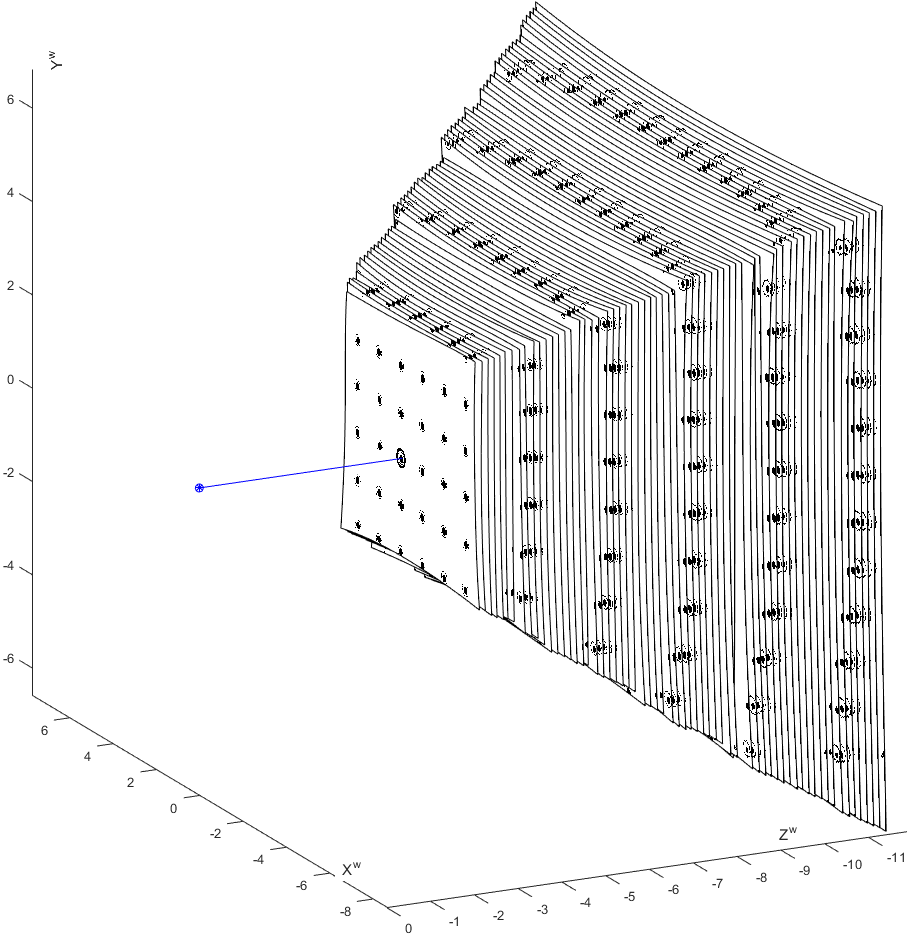
\includegraphics[width=0.7\textwidth, height= 0.55\textwidth]{Data63FranesForLUT}
\caption{63 Frames NearIR Rectified 3D Reconstruction}
\label{Data63FranesForLUT}
\end{figure}%
%
Figure \ref{Data63FranesForLUT} shows 63 frames of NearIR rectified 3D reconstruction, which gives an intuitionally pyramid shape of a camera sensor's field of view. The pyramid is composed of all of the pixel-beams, every single one of which could be expressed as \\%
%
\begin{equation}
%
\begin{aligned}
X(col, \, row) &= c_{(col, row)}Z(col, \, row)+d_{(col, row)}
\\%
Y(col, \, row) &= e_{(col, row)}Z(col, \, row)+f_{(col, row)}
\end{aligned}
\label{fromZ_To_XY}
%
\end{equation}%
%
where \({(col, row)}\) denote the address of a pixels, \(c\)/\(d\)/\(e\)/\(f\) are the corresponding linear coefficients that help map from \(Z\) to \(X\) and \(Y\).%
\\\\%
Figure \ref{SampleBeams_NearIR} shows some sample beams composed of coefficients \(c\)/\(d\)/\(e\)/\(f\), which gives a rectified field of view. It explains the lens distortions affections, that those beams are converged in front of the origin.\\%
%
\begin{figure}[h]
\centering
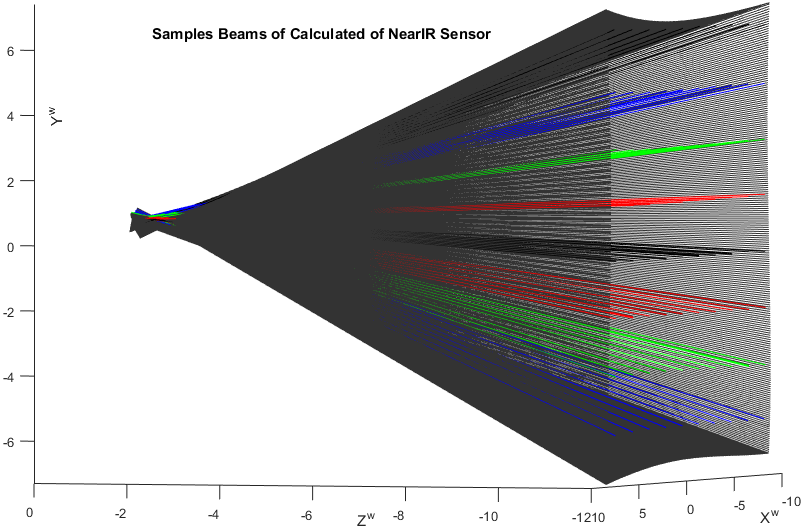
\includegraphics[width=0.77\textwidth]{SampleBeams_NearIR}
\caption{Sample Beams of Rectified NearIR Field of View}
\label{SampleBeams_NearIR}
\end{figure}%
\\%
To combine equation \ref{fromD_To_Z} and \ref{fromZ_To_XY}, a rectified 3D coordinate (\(X\), \(Y\), \(Z\)) for every single pixel could be looked up based on \(D\). With enough data generating a  \(column\)-by-\(row\)-by-\(6\)  look-up table that contains 6 coefficients (\(a\),\(b\),\(c\),\(d\),\(e\),\(f\)) for every single pixel, a rectified real-time 3D reconstruction could be displayed.
%
\section{Real-Time analysis}
Real-time analysis is in contrast with off-line process. In terms of camera steams process, real-time means to display the first processed frame before the second frame processing starts. In this thesis, \enquote{real-time} could be used to describe both of the 3D rectification procedure for Look-Up Table (LUT) generation and the live show of calibrated observation using LUT.
\subsection{Real-Time in Rectification}
In the process of 3D (\(X^{w}\),\,\(Y^{w}\),\,\(Z^{w}\)) rectification using an uniform grid dots pattern, \enquote{real-time} means being able to show a rectified frame, as well as to record its rectified \(XYZWRGBD\) steams data, before the start of second frame processing. The recored frames (\(XYZWRGBD\)s) will be used to generating LUT.%
\\\\%
With the help of the BLE Optical-Flow tracking module, which will be discussed in section \ref{BLE_OF_TrackingModule}, this rectification step could really be called \enquote{real-time}: not only \(X^{w}\) and \(Y^{w}\) are rectified before the coming of the next frame, but also \(Z^{w}\) is updated (at a rate of 100Hz, maximum 5KHz) as the slider moving along the rail (along \(Z\)-axis). After an appropriate setting, a group (concretely, 63 frames) of rectified \(XYZWRGBD\) steams data could be recorded automatically as the slider moving (record one rectified frame at every 25mm) from the head of the rail to the tail, as already shown in figure \ref{Data63FranesForLUT}.%
\\\\%
The processing speed depends on the number of detected dot-clusters. The further where the camera is observing the dots pattern, the more dot-clusters are detected, the slower processing speed will be. In practical, the real-time rectification speed 4 fps at the head of the rail (working distance 1.05m), and 0.4 fps at the end of the rail (working distance 2.7m).
%
\subsection{Real-Time Observing after Rectification}
%
For the live-show of observed steams after rectification, the camera's view is no longer limited by the uniform grid pattern. At that time, \enquote{real-time} means to look up the rectified (\(X^{w}\),\, \(Y^{w}\),\, \(Z^{w}\)) based on \(D\) and read its corresponding RGB for every single pixel, and then show the reconstructed 3D image, before the next frame.%
\\\\%
Concretely, for every single pixel, 6 coefficients (\(a\),\(b\),\(c\),\(d\),\(e\),\(f\)) will be looked up, and their corresponding \(Z^{w}\) and \(X^{w}\)/\(Y^{w}\) will be determined by equation \ref{fromD_To_Z} and equation \ref{fromZ_To_XY}.
%
%
%\section{3D Reconstruction differences for PrimeSense, KinectV2, and Prosilica}
%pixels, steams, and shader comparison
%
%
%
%
%
%
%































 
% Chapter 3
\chapter{Calibration System for RGBD Cameras} % Main chapter title
\label{sens_CalibrationSystem} % For referencing the chapter elsewhere, use \ref{sens_CalibrationSystem} 
%
%
\section{Rail System}%
As already shown in chapter \ref{sens_introduction} figure \ref{trackingModuleOnKinectV2CalibrationSystem}, the whole calibration system consists of an RGB-D camera, a plane of round dot pattern, rail, and a BLE Optical-Flow tracking module. 
Other than the round dot pattern standing in front of the 3D camera for offering distortion information, all of the rest parts of the whole calibration system are centered on the rail, which is made with 80/20s. Taking the round dot pattern plane as plane \(X^wY^w\), the rail is placed right perpendicular to the dot pattern along the direction of \(Z^w\) axis. Both of the RGB-D camera and the BLE Optical-Flow tracking module are mounted on the slider of the rail. \par
%
Sitting on the top of the elevated carriage of the slider, the RGB-D camera's vision keeps being horizontal, parallel with \(Z^w\) axis. And the origin is chosen right at the center of the camera's field of view, like figure \ref{cameraFieldOfView} shows.\par
%
\begin{figure}[h]
\centering
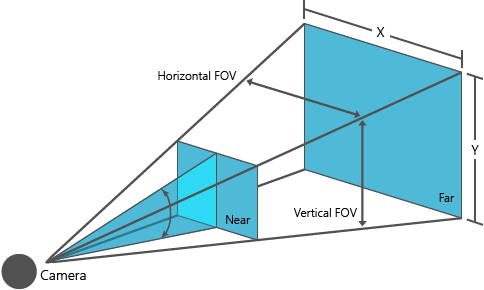
\includegraphics[width=\textwidth]{cameraFieldOfView}
\caption{World Coordinate Frame}
\label{cameraFieldOfView}
\end{figure}%
%
The BLE Optical-Flow tracking module is mounted at the bottom of the rail to tracking the movements of the slider, as shown in figure \ref{MountedTrackingModuleObservingRail}. With infrared LED projecting injective rays onto the inner surface of the 80/20 groove, Optical-Flow sensor could generate accumulated X/Y value based on its observed optical flow changes (the changes of diffuse reflection rays from inner surface, generated by LED). The white re-stickable strip covering on the joint between PCB and OF sensor is for shocking absorption. Sliding along the rail, the accumulated Y value is always zero, and the accumulated X value records the movements of the slider, and will be sent into PC over the air by the BLE module. 
%
\par
%
\begin{figure}[h]
\centering
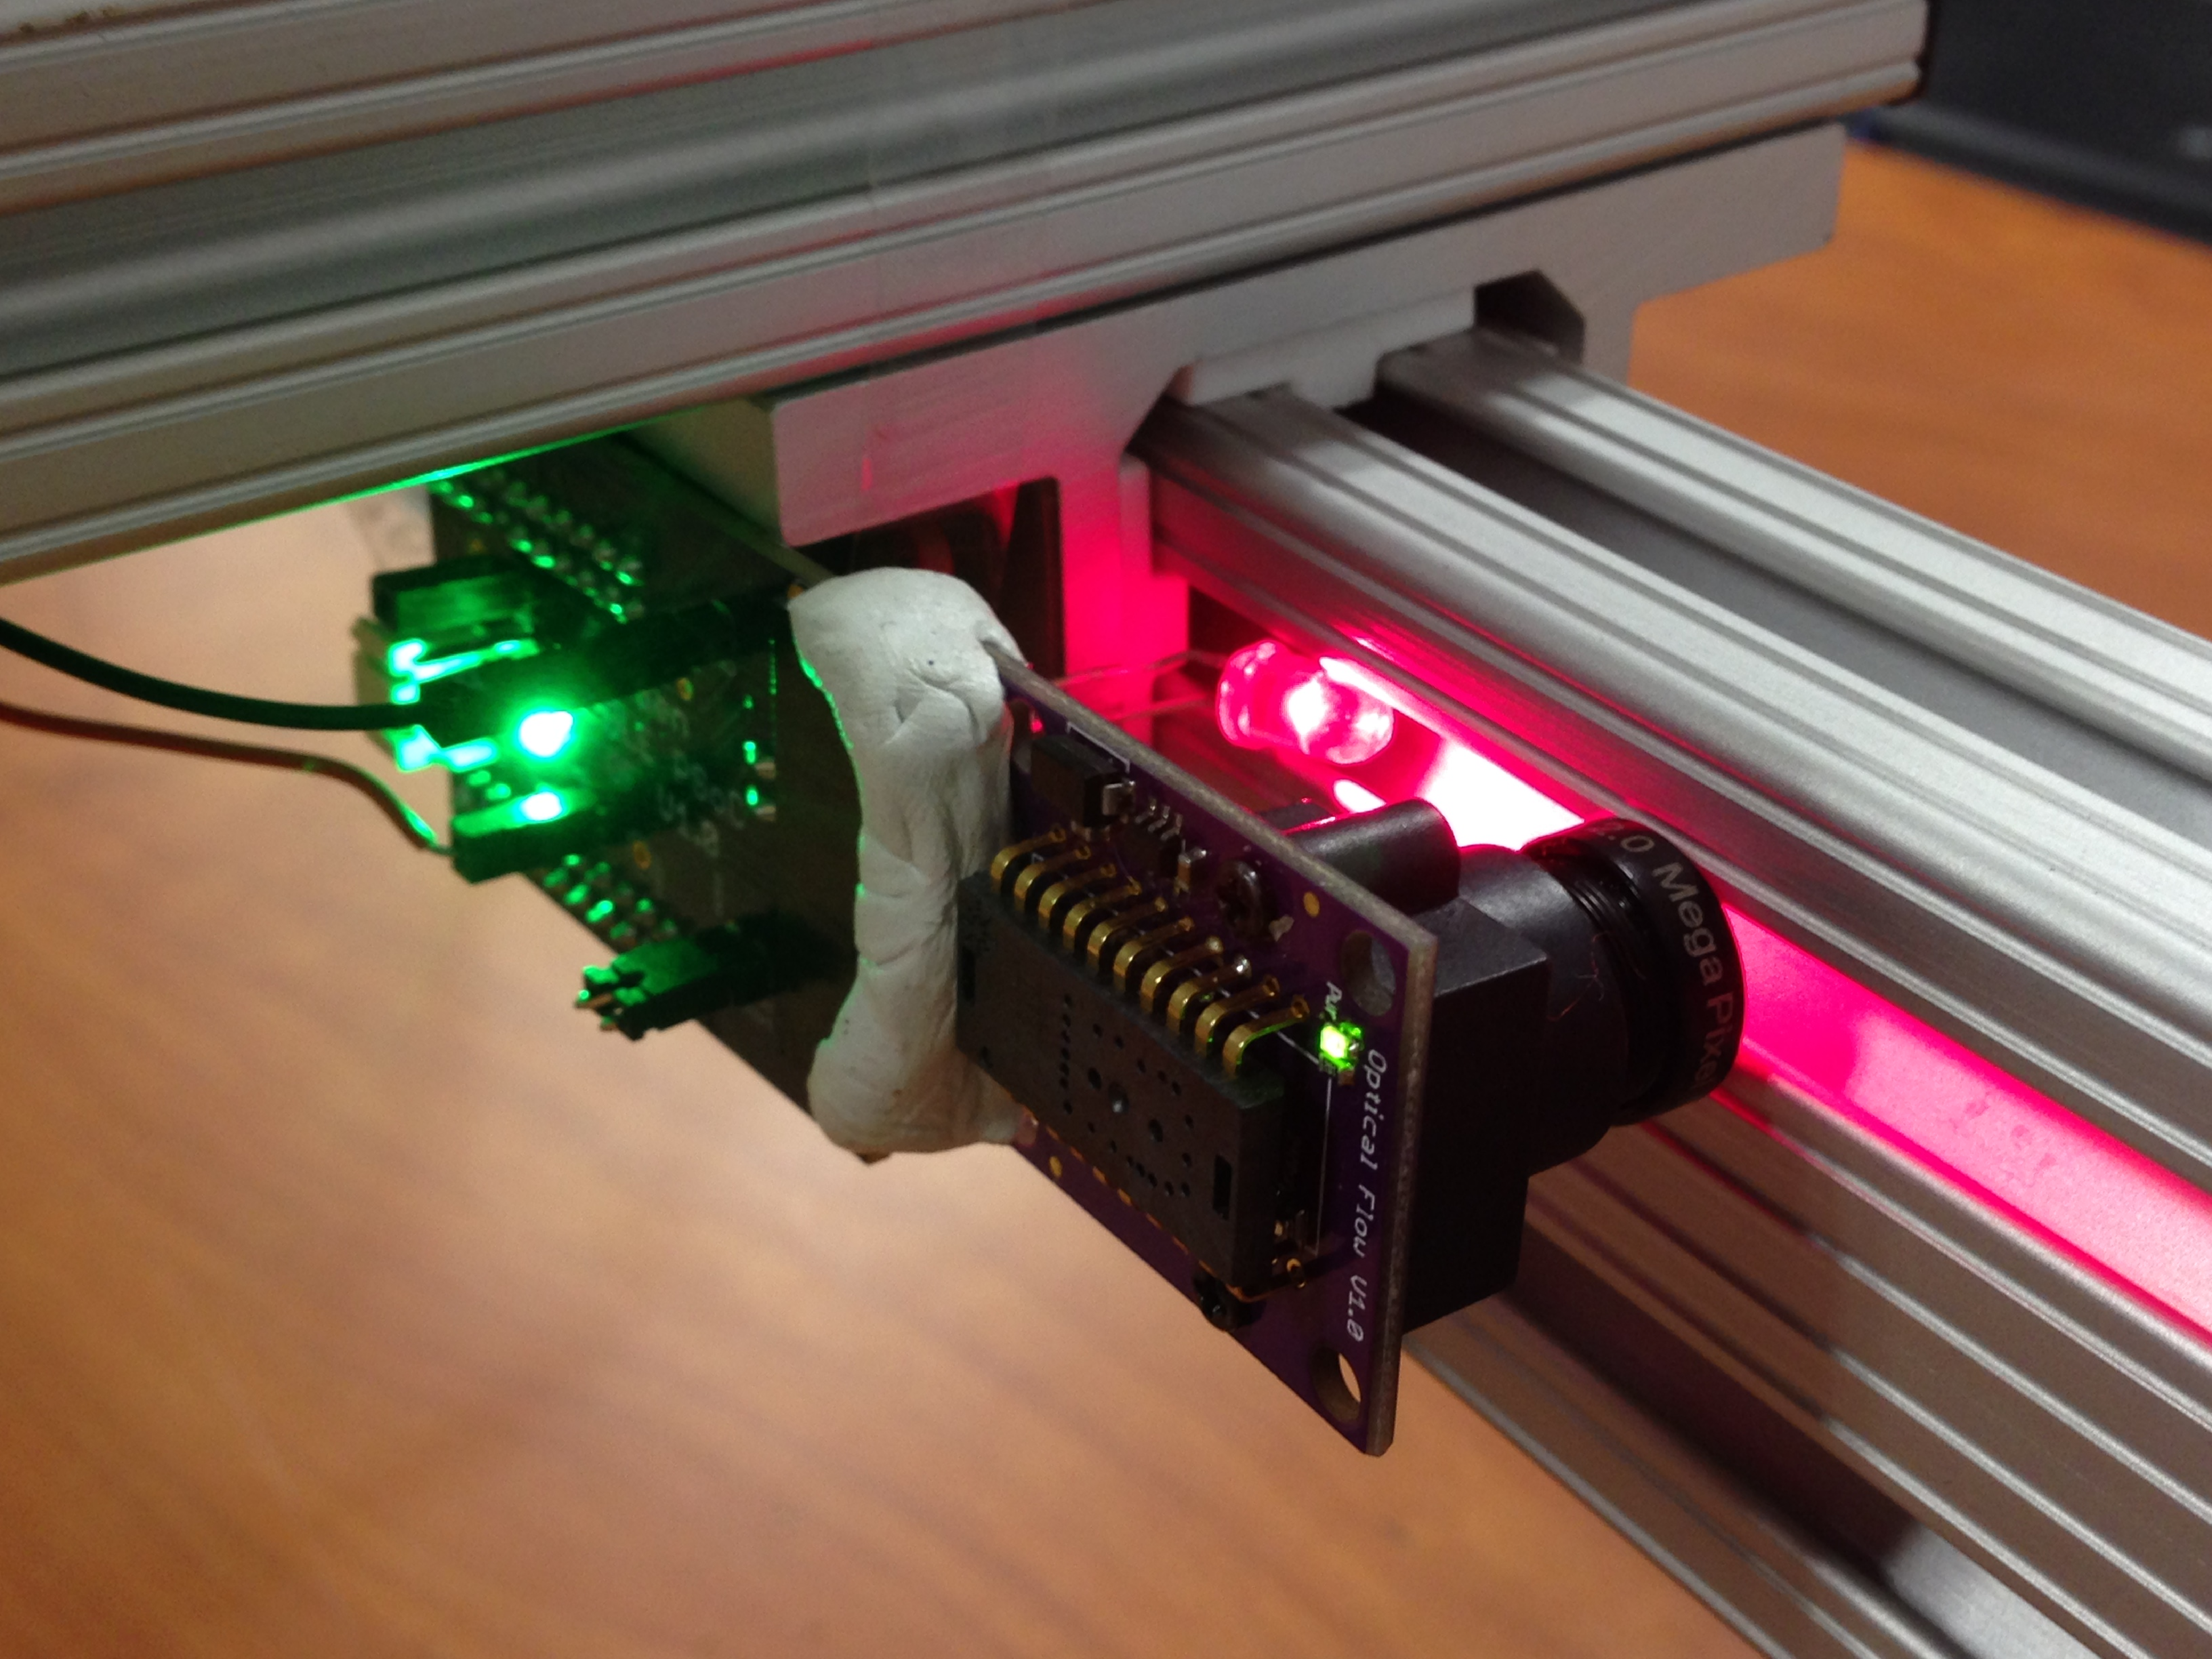
\includegraphics[width=0.85\textwidth]{MountedTrackingModuleObservingRail}
\caption{Mounted BLE Optical-Flow Tracking Module}
\label{MountedTrackingModuleObservingRail}
\end{figure}%
%
%
%
\section{BLE Optical-Flow Tracking Module}
\label{BLE_OF_TrackingModule}
%
The BLE Optical-Flow tracking module consists of an Optical-Flow sensor for movement detection, a LED for illumination, a PSoC BLE module for wireless data communication, and a self-designed PCB as a joint.
%
\subsection{Optical-Flow Sensor for Z Tracking}
%
\enquote{Optical-Flow} depicts the motion of brightness patterns. In daily life, optical flow is continually processed in our visual system, offering the estimations informations of self-motion, relative depths, object speed, etc. Whereas in computer vision, optical flow is digitally saved as the motion vector for every voxel position, telling about the relative distances of objects in a given sequence of images.%
%[1] J.L. Barron and N.A. Thacker, "Tutorial: Computing 2D and 3D Optical Flow", Tina Memo No. 2004-012, 2005. 
\\\\%
For the rail system tracking on the slider along \(Z\)-axis, using optical flow for motion detection is one the best choice in the non-contact motion tracking methods. 
%
\subsubsection{Optical-Flow Motion Determination}
%
The optical flow methods calculate the motion between every two image frames which are taken at times \(t\) and \( t+\Delta t\) at every voxel position. %
%S. S. Beauchemin; J. L. Barron (1995). The computation of optical flow. ACM New York, USA.
Even though there are various algorithms 
%https://en.wikipedia.org/wiki/Optical_flow#cite_note-S._S._Beauchemin_.2C_J._L._Barron_1995-6
using optical flow to determine motion, they are all based on the Brightness Constancy Constraint, which in \(2D+t\) dimensional camera case can be written as 
%
\begin{equation}
%
I(x, \, y, \, t) = I(x + \Delta x, \, y + \Delta y, \, t + \Delta t)
%
\end{equation}
%
where (\(x\), \(y\), t) denotes the location of a voxel, \(I(x, \, y, \, t)\) is its corresponding intensity; \(\Delta x\) and \(\Delta y\) are the changes between two frames taken at time \(t\) and time \(t + \Delta t\).%
\\\\%
An optical flow sensor is a vision sensor capable of measuring optical flow or visual motion and outputting a measurement based on optical flow. In this project, we use a optical mouse sensor, whose vision chip is integrated circuit that have both an image sensor for vision and a processor running one programmed optical flow algorithm in one compact implementation. As shown in figure \ref{OpticalFlowSensor}, optical mouse sensor ADNS-3080 is used practically.
%
\begin{figure}[h]
\centering
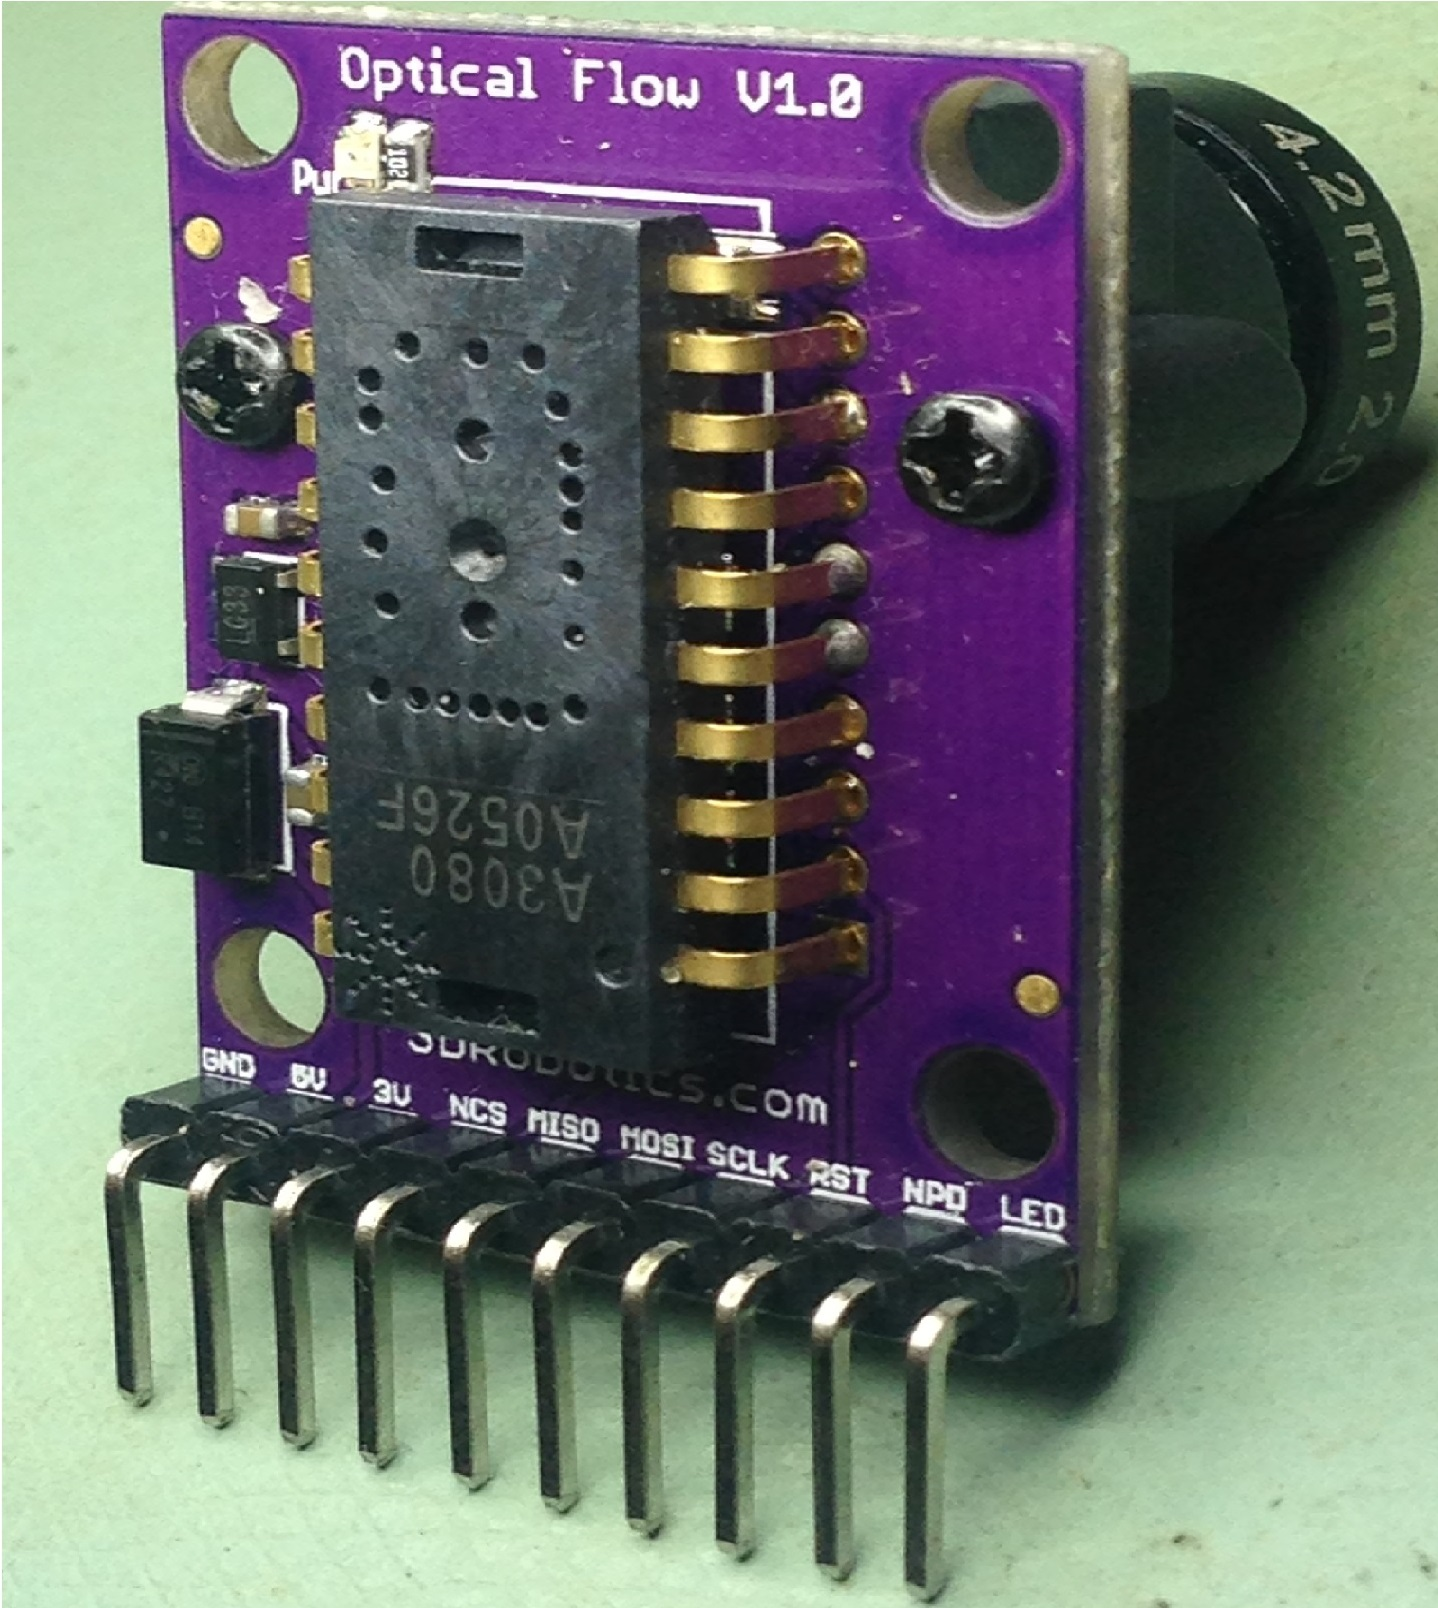
\includegraphics[width=0.4\textwidth]{OpticalFlowSensor}
\caption{Optical Mouse Sensor}
\label{OpticalFlowSensor}
\end{figure}%
%
\subsubsection{Accumulated \(Z^w\)-axis data calibration}
%
Sensor ANDS-3080 has a programmable frame rate of over 6400 fps. With a lens mounted, this optical flow sensor can theoretically adjust its working distance from zero to one meter. Both of the raw 30-by-30 image frame and the calculated motion results could be retrieved from the optical flow sensor in two different working modes. In the \enquote{image burst} mode, the raw 30-by-30 image frames form a 10 fps live video, helping adjust the lens for a better focus. Whereas in the \enquote{motion burst} mode, the calculated motion results offers accumulation data for both of the sensor's \(x\)-axis and \(y\)-axis.
\\\\%
Concretely as shown in figure \ref{MountedTrackingModuleObservingRail}, only the \(y\)-axis accumulated data is used as the accumulated \(Z^w\)-axis data in the world coordinate, whereas the \(x\)-axis accumulation is always zero (no motion on the \(x\)-axis. Employing the \enquote{motion burst} mode, on ever update, the world coordinate \(Z^w\) could be written as%
%
\begin{equation}
%
Z^w = Z^w_0 + ratio*y^{acc} = Z^w_0 + ratio*(y_{\text{\_all\_previous}} + y_{\text{\_new\_updated}})
%
\end{equation}
%
where \(Z^w_0\) denotes the beginning point of accumulating (concretely at the closest end of the rail to dots pattern), \(ratio\) maps the \enquote{unit one} from \(y\)-axis to the \(Z^w\)-axis, \(y^{acc}\) denotes the accumulated \(y\)-axis movement by data retrieved from the optical flow sensor, which equals to the sum of all previous values and the new updated value.
%
\subsection{Bluetooth Low Energy for wireless communication}
%
ZigBee, Bluetooth, and Bluetooth Low Energy (BLE) are three most commonly used Personal Area Network (PAN) wireless standards to choose from when wireless communication is needed. ZigBee runs on a mesh topology network (star and point-to-point are the other two basic topologies), which means that the information travels on a web of multiple nodes. Whereas Bluetooth and BLE are famous as point-to-point networking standard, which suits better for this project, from Optical-Flow sensor to PC.
\\\\%
There are huge differences between BLE and \enquote{classic} Bluetooth; despite falling under the same name, they are entirely different technologies. Bluetooth consumes more power and transmits farther and with more data. It is suited for streaming media such as playing music on Bluetooth speakers or taking a call through a Bluetooth headset.
%
\begin{figure}[H]
\centering
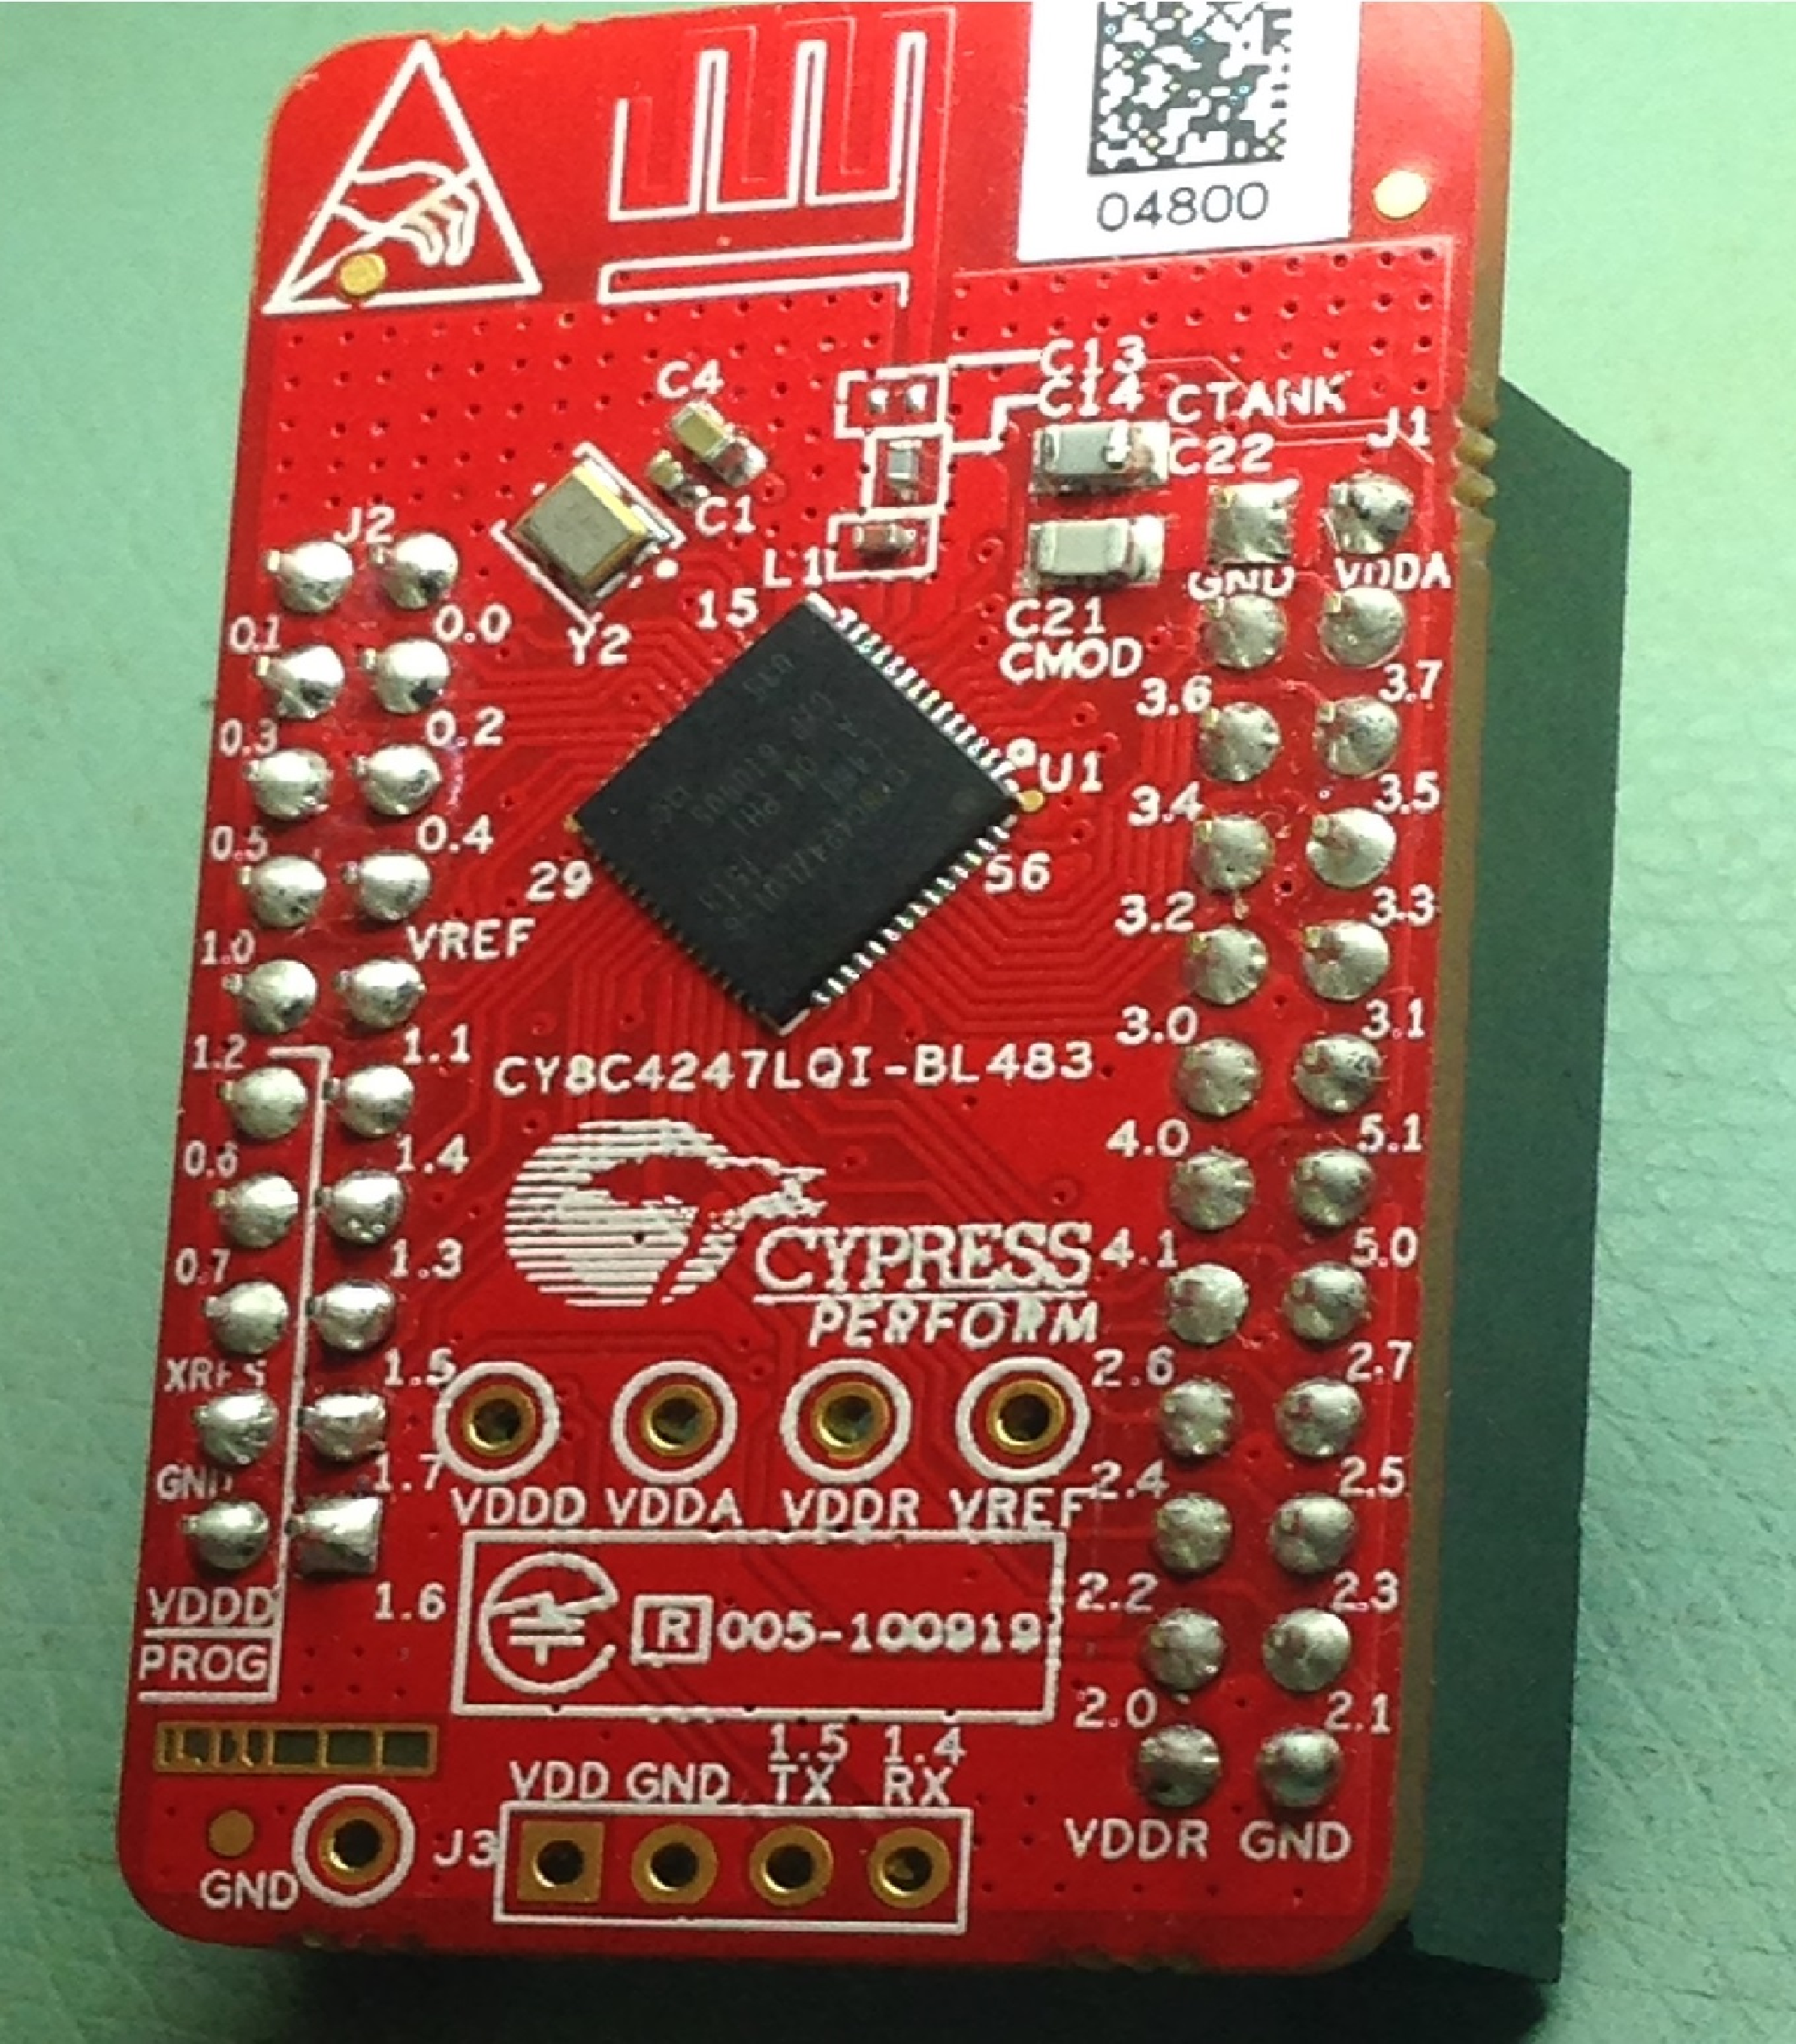
\includegraphics[width=0.4\textwidth]{PSoC_BLE_Module}
\caption{Cypress PSoC BLE Module}
\label{PSoC_BLE_Module}
\end{figure}%
%
Whereas BLE transmits less data over shorter distances using much less power than Bluetooth. Both of the transmission frequency and the amount of data to transfer per time are controllable by developer for BLE communication.
\\\\
%
As for the wireless data transmission in this project, with the \(x\)/\(y\) accumulation data being to transfer, the amount of data to transfer per time is only two bytes. Moreover, the maximum frame rate of optical flow sensor ANDS-3080 is 6400 fps, which means the transmission frequency cannot be faster than 6400 Hz (we do not need that fast in the meantime). In short, BLE is finally chosen as the wireless networking to transfer data from the optical flow sensor to PC. Concretely, the Cypress PSoC BLE Module is used, with a 10KB maximum throughput that is enough for the demand in this project, as shown in figure \ref{PSoC_BLE_Module}.
%
\subsubsection{BLE Programming based on Protocol}
%
BLE is a low-power, short-range, low-data-rate wireless communication protocol. Unlike Bluetooth application that only the high level connection needs to be concerned, the BLE application developing needs low level programming, more complex but offering more control space for developer. Figure \ref{BLE_Protocol_Stack} shows the BLE Protocol Stack that BLE developers need to refer to.
%
\begin{figure}[H]
\centering
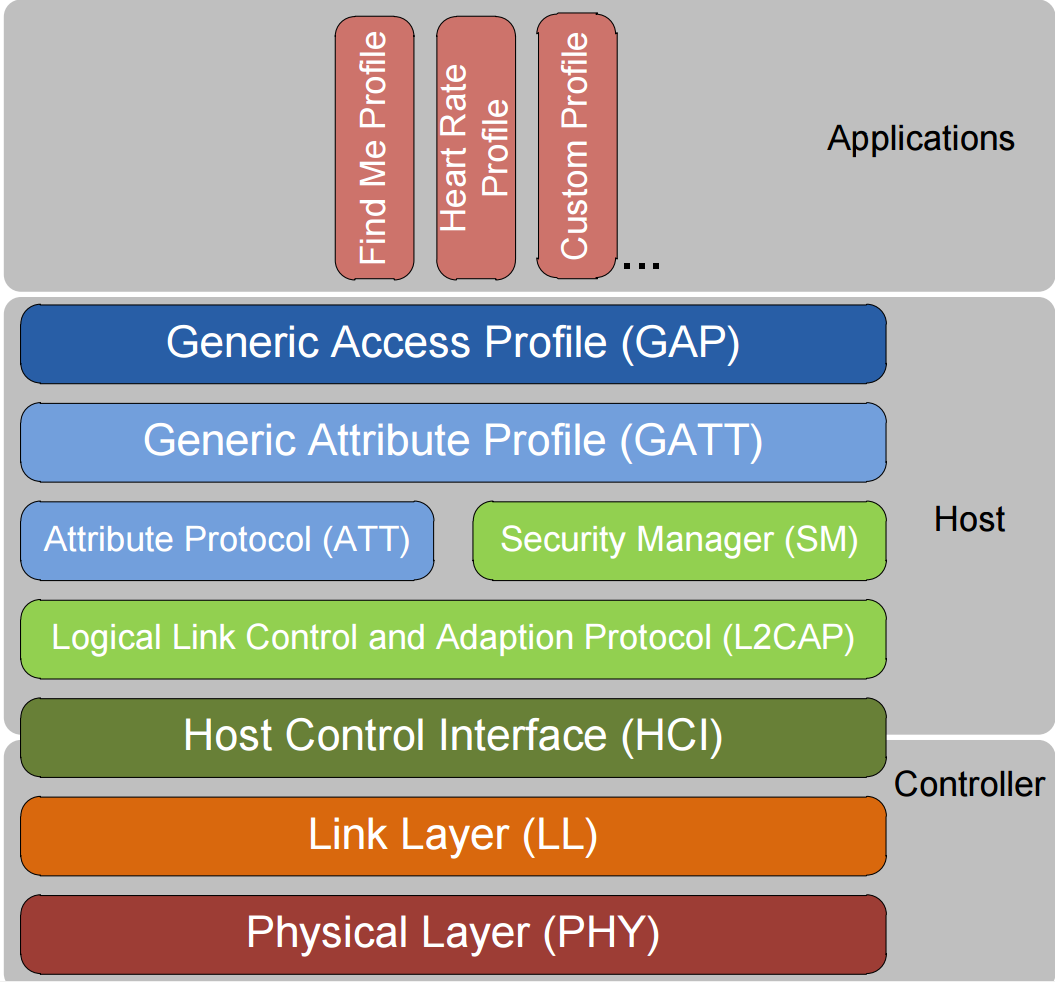
\includegraphics[width=0.7\textwidth]{BLE_Protocol_Stack}
\caption{BLE Protocol Stack}
\label{BLE_Protocol_Stack}
\end{figure}%
%
Cypress BLE Module helps handle the lowest hardware controller section (PHY, LL, HCI) and part of the firmware host section (L2CAP, ATT, SM), so that developers only need to take care of the GAP and GATT layers. GAP provides an application-oriented interface that determines whether the device acts as a BLE link \enquote{Central} or \enquote{Peripheral}, and configures the underlying layers accordingly. Whereas GATT defines methods to access data defined by ATT layer ( \enquote{Client} to receive or \enquote{Sever} to send).
\\\\%
Concretely for the BLE programming in this project, on the GPA layer, the BLE module continuously retrieving data from Optical-Flow sensor is the \enquote{Peripheral} that advertises to a Central, while a BLE dongle (receiver connected on PC) is the \enquote{Central} that scans for advertisements from GAP Peripherals and is going to establish the connection with the BLE module. Whereas on the GATT layer, the BLE module is the \enquote{Sever} that contains data and the dongle on PC works as a \enquote{Client} to receive data.
\\\\%
To program on the PC side, both of the command sending and data receiving are through the serial port which connects the BLE dongle. Both of the output command to send and received the input data are packaged in a center format, which means for every command about BLE control, there must be a method to package it and a corresponding decoding method to extract valid data. All of the commands that need to be managed are to handle GATT data transmission and GAP connection problem. After GATT and GAP setting, concretely, the optical flow sensor works at a sampling rate of 2000Hz and the BLE communication speed is 100 updates per second, i.e., \(Z^w\) is updated at 100Hz.
%
%
\subsection{PCB Joint, Power Supply and Illumination}
%
Figure \ref{SenSinglePCB} shows the PCB combining and powering (3.3 \texttildelow \, 16V flexible voltage input) for a PSoC BLE module, an OF sensor, and a LED for OF sensor illumination. Figure \ref{BLE_OF_TrackingModule_Overview} shows the overview of the BLE Optical-Flow Tracking Module.
%
\begin{figure}[H]
\centering
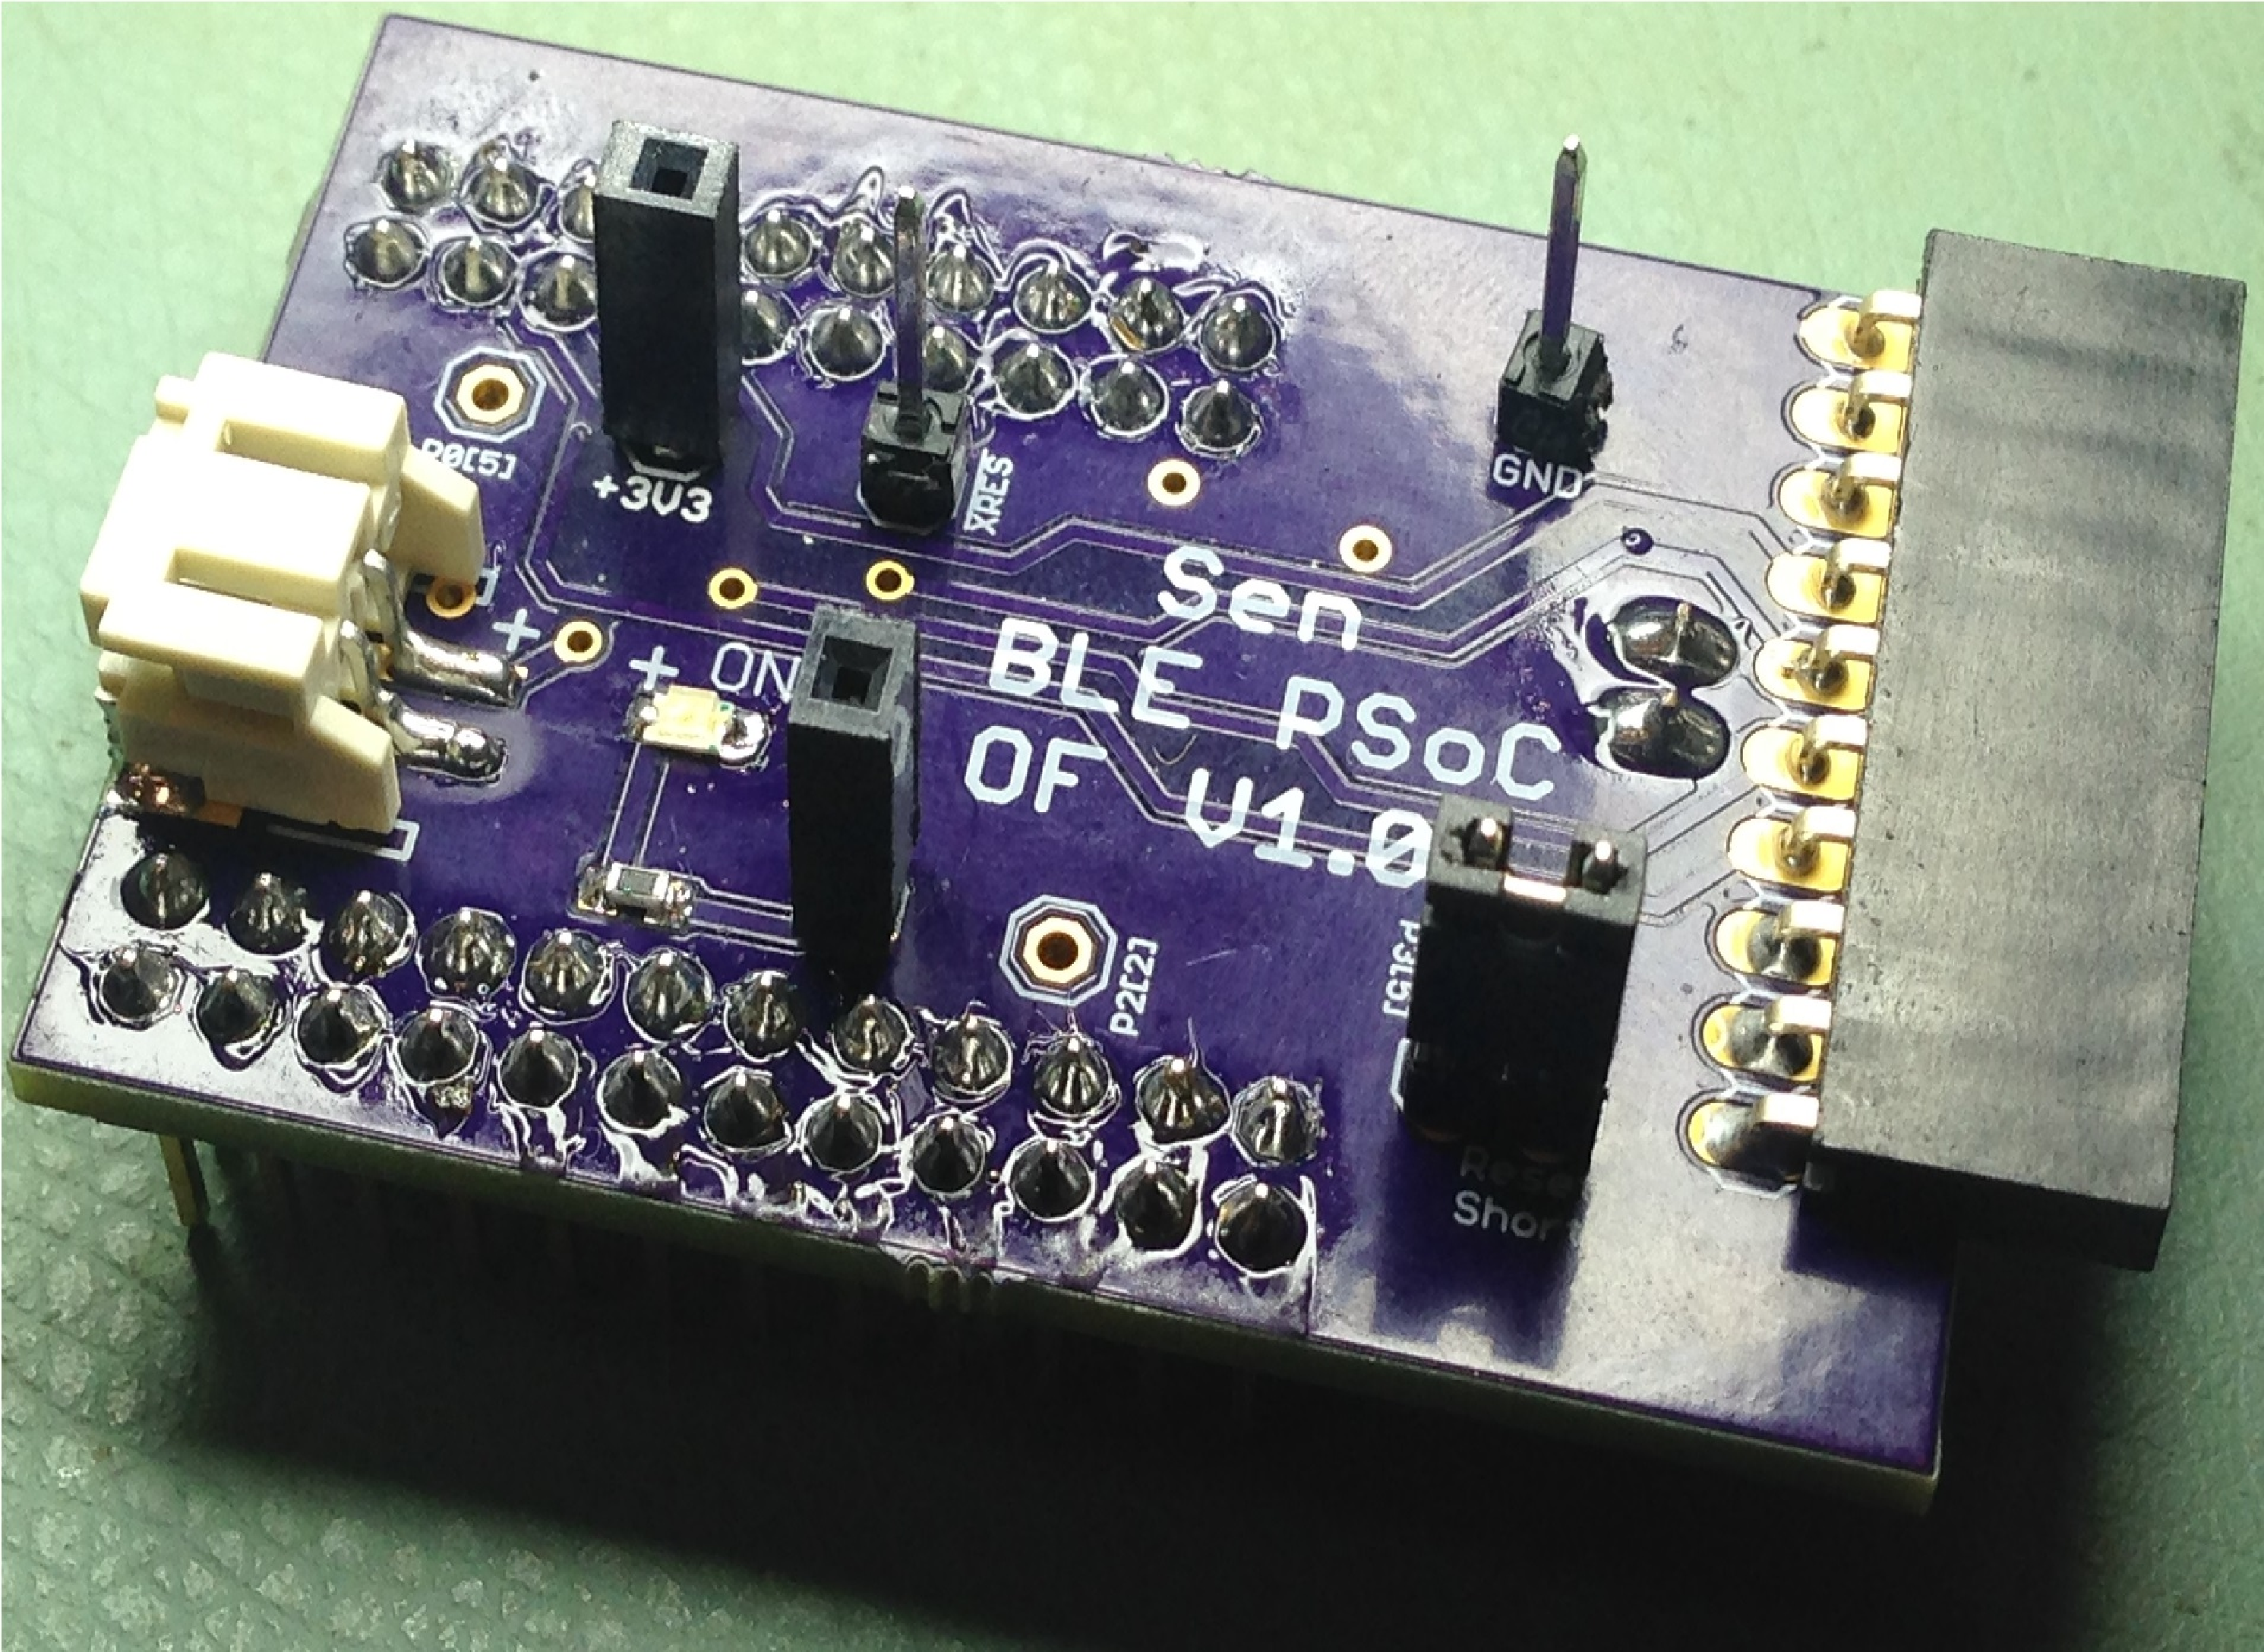
\includegraphics[width=0.7\textwidth]{SenSinglePCB}
\caption{PCB: joint \& power supply}
\label{SenSinglePCB}
\end{figure}%
%
%
 \begin{figure}[H]
\hspace*{-0.3cm}
\centering
\subfloat[Front Side][Front]{
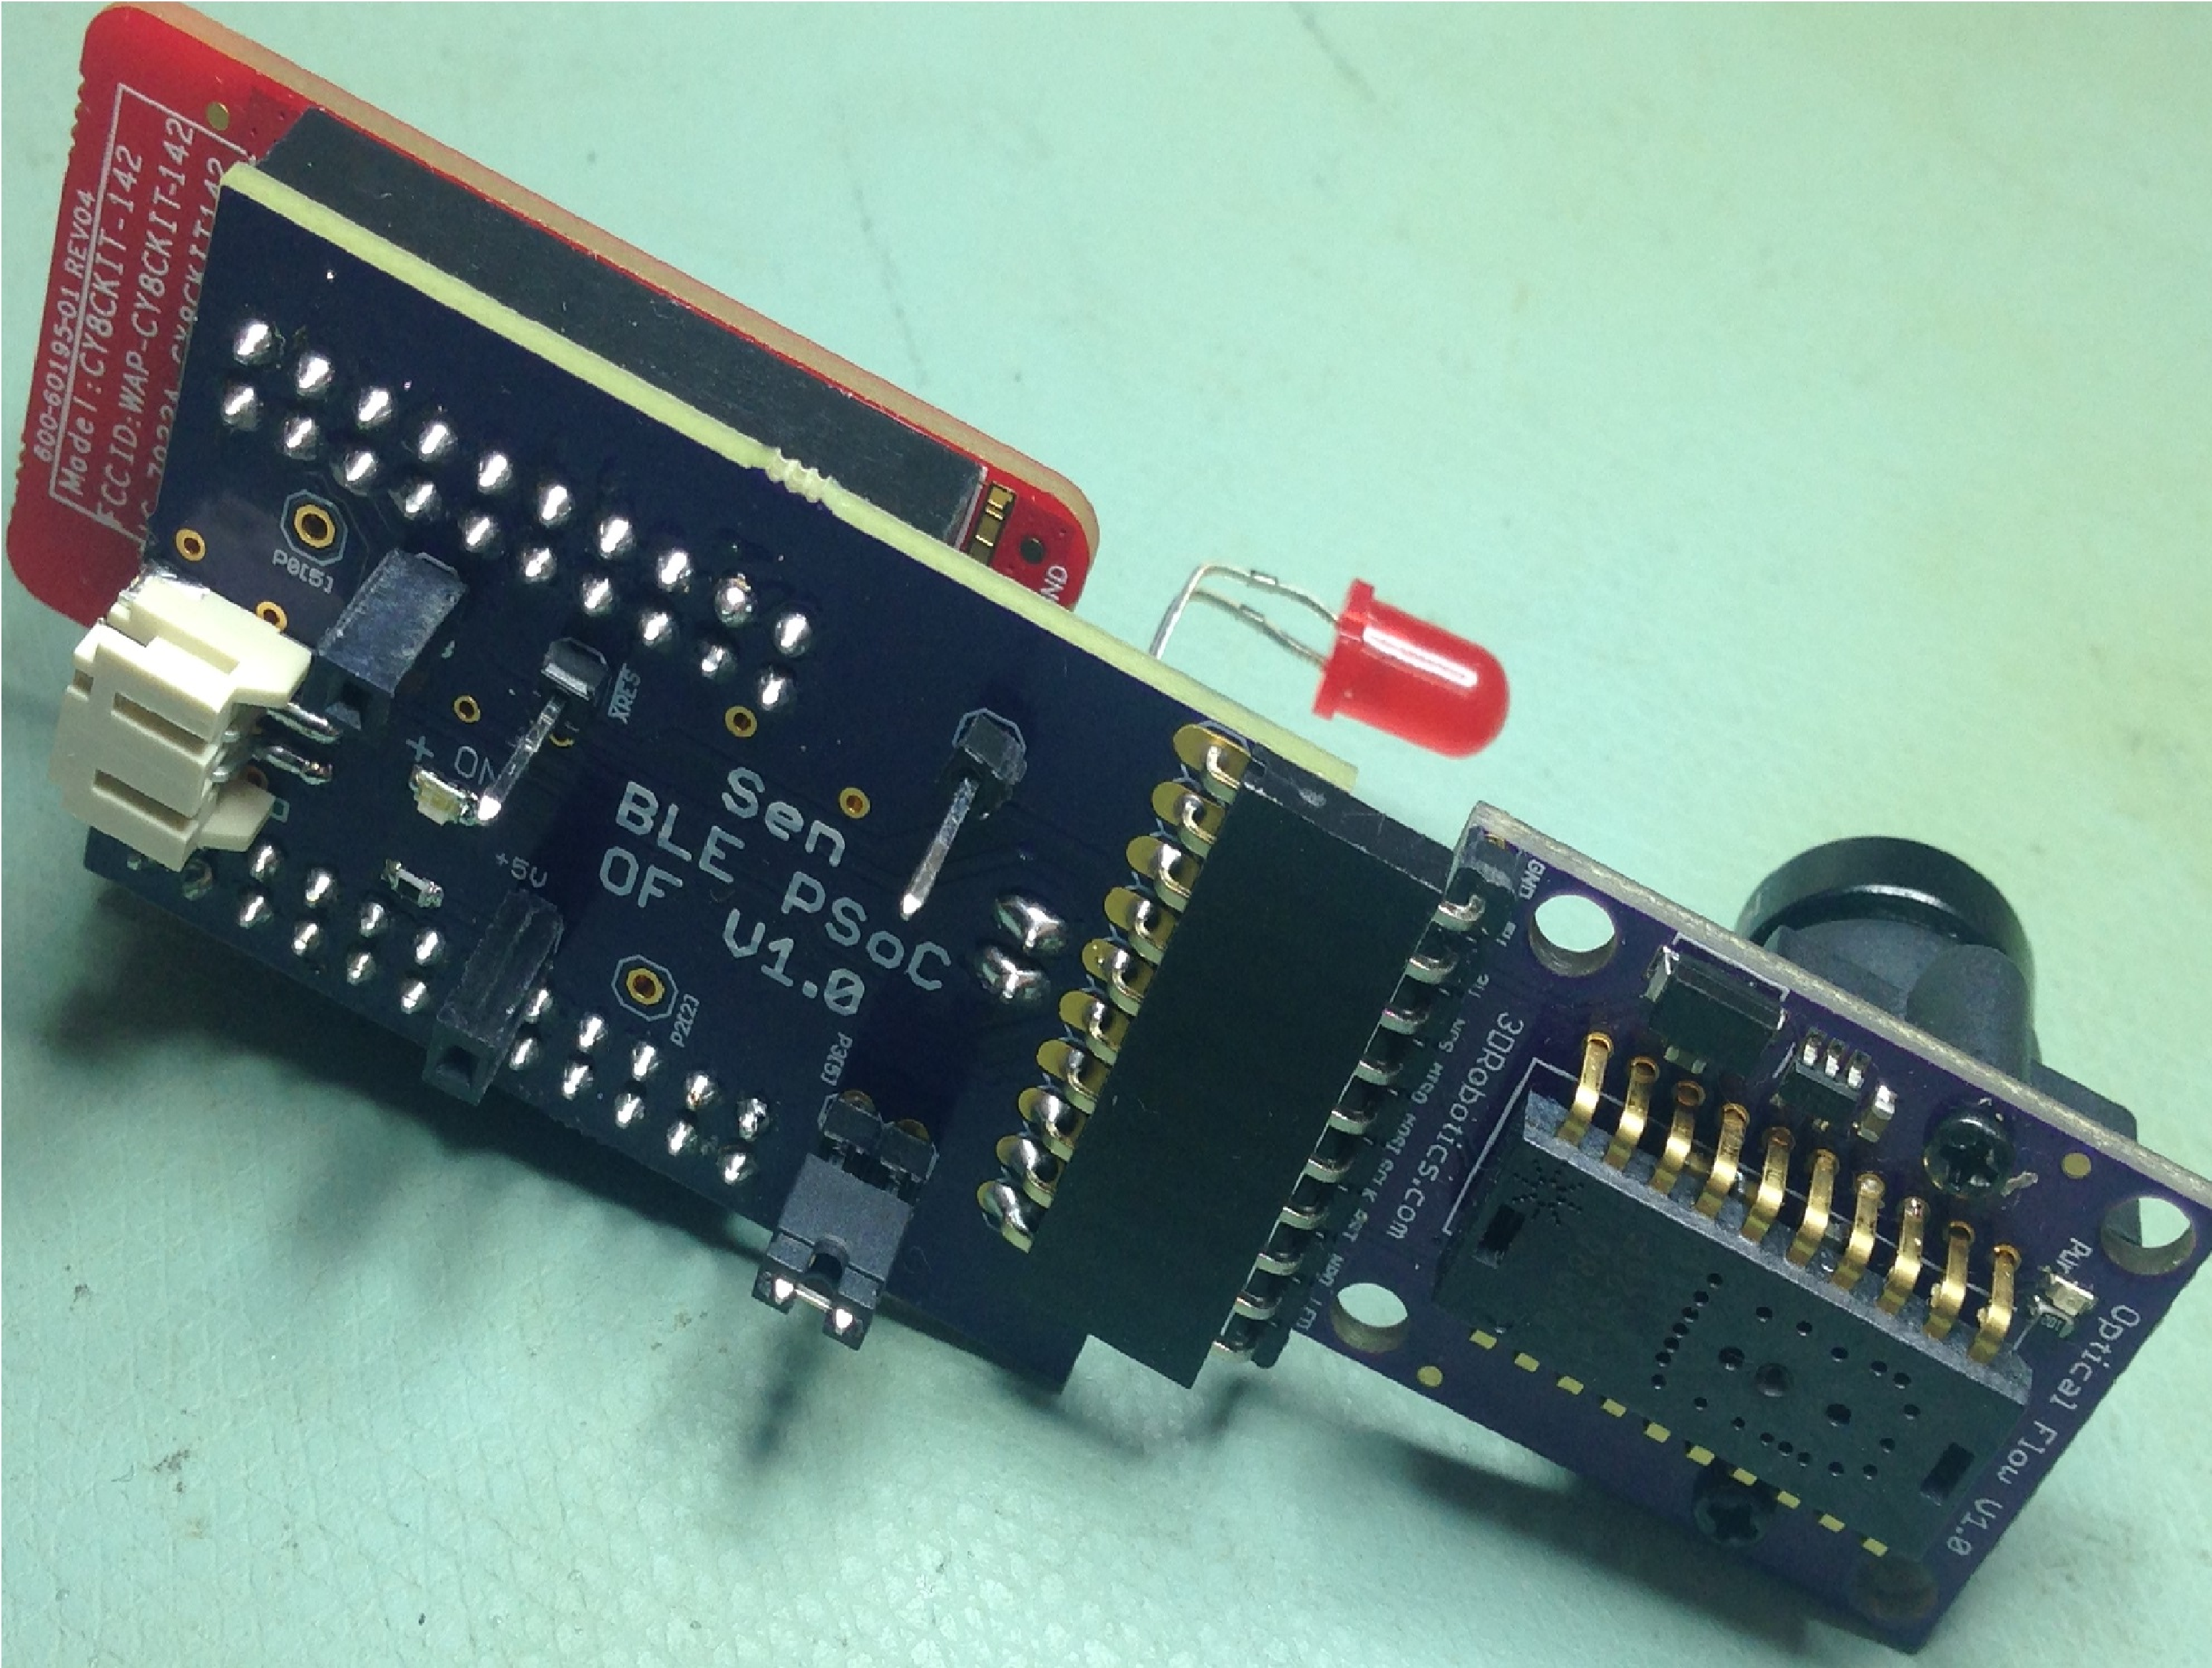
\includegraphics[width=0.54\textwidth, height = 0.35\textwidth]{combinedModuleFace}
\label{combinedModuleFace}}
%\qquad
\subfloat[Back Side][Back]{
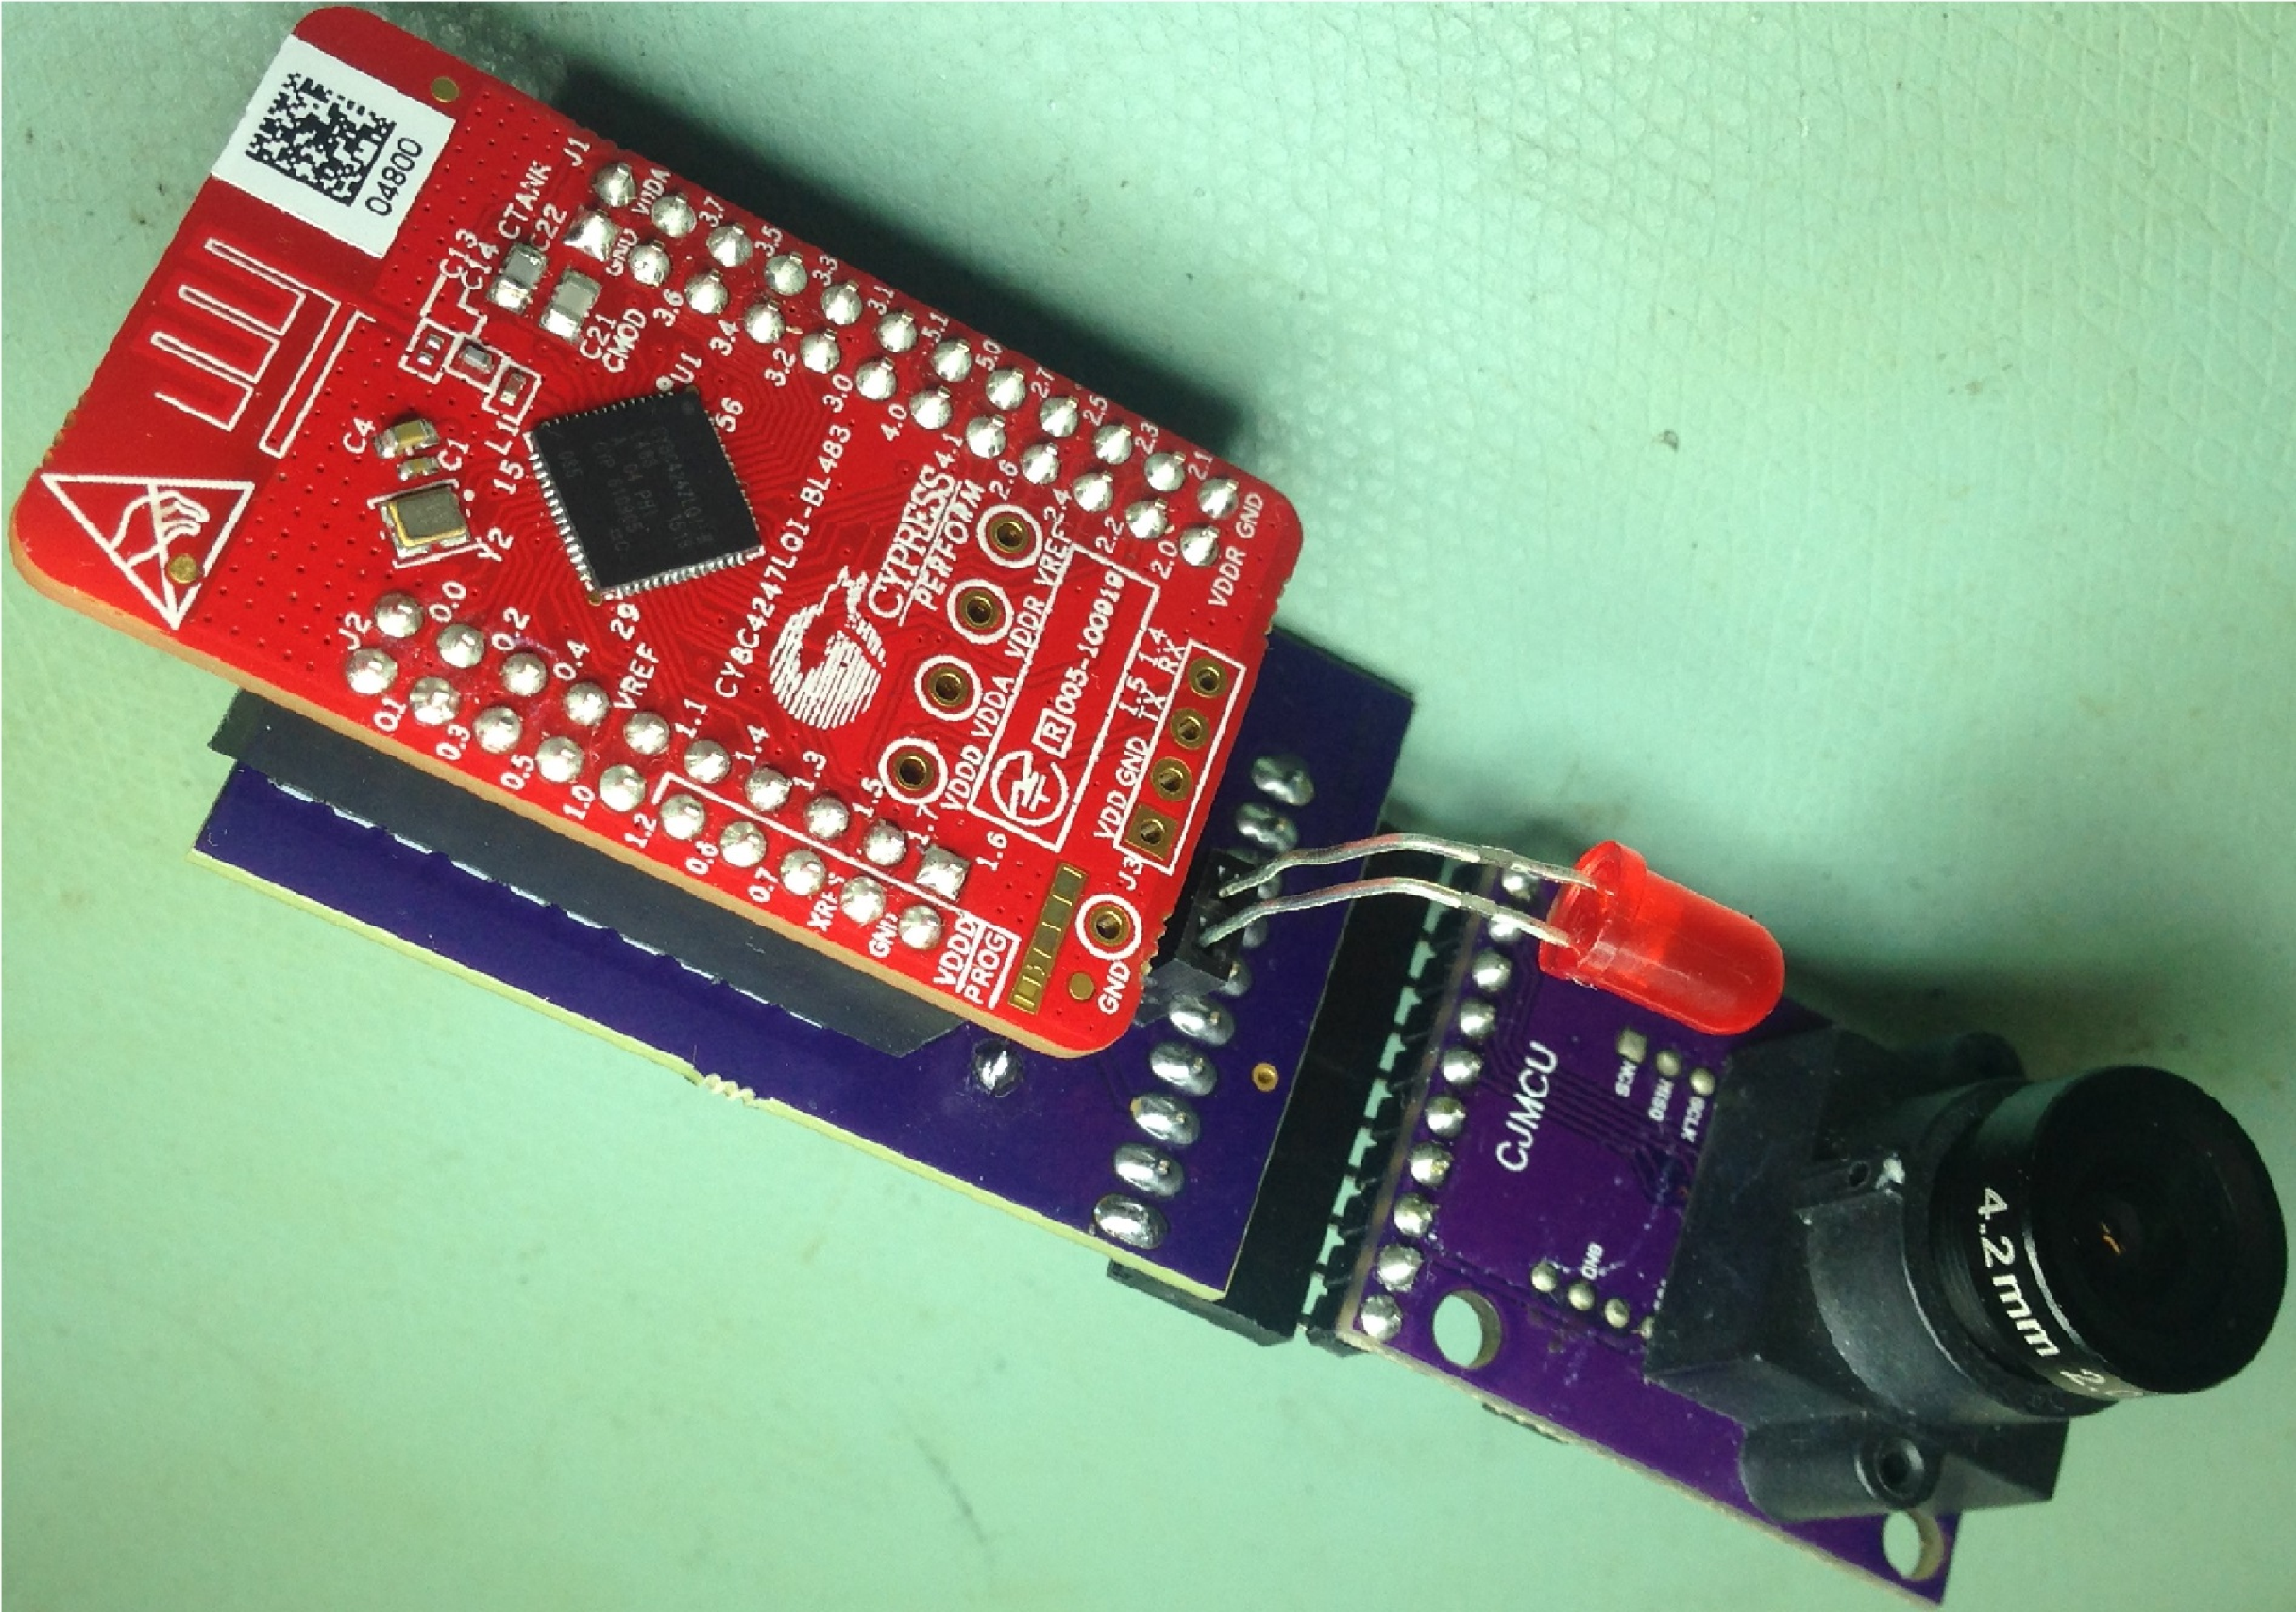
\includegraphics[width = 0.47\textwidth, height = 0.35\textwidth]{combinedModuleBack}
\label{combinedModuleBack}}
%
\caption{Overview of BLE OF Tracking Module}
\label{BLE_OF_TrackingModule_Overview}
\end{figure}%
%
%
%
%
%
%
%
%Chapter 4: results for 3 types of RGB-D cameras.\\
%Chapter 5: conclusion\\






































%% Chapter 3
\chapter{Conclusion and Future Work} % Main chapter title
\label{sens_ConclusionAndFutureWork} 
%
RGB-D cameras have both of lens distortions and depth distortion problem. Distortions correction is wildly discussed in image processing area. In this thesis, a data-based LUT software calibration method for general RGB-D cameras is proposed, in contrast with the pinhole-camera-model based traditional method. In this section, both of the advantages and and disadvantages are concluded, and the possible avenues of future study are discussed.
%
\section{Conclusion}
In traditional 3D cameras' calibration, 3D reconstruction (based on pinhole camera model) and lens distortion are separated, which depresses the efficiency of image processing. Moreover, it does not include the depth distortion correction, assuming that the depth values are accurate and employing them directly as \(Z^w\) in 3D reconstruction.%
\\\\%
In stead of using a pinhole camera model, which in practical is not ideally accurate, our new proposed calibration method is based on real data. Not only \(X^w\)/\(Y^w\) values are rectified directly through one step transformation, but \(Z^w\) is also guaranteed accurate by importing externally measured data. 
\\\\%
During this data-based calibration method, high-order polynomial surface mapping is employed for \(X^w\)/\(Y^w\) rectification, as discussed in section \ref{sectionHighOrderPolynomialSurfaceMapping}. And an IoT technology, an individual BLE OF tracking module is introduced for the support of external \(Z^w\) data, offering a way for the depth distortion correction.
\\\\%
In contrast with the traditional pinhole-camera-model based method, the new proposed data-based method offers more efficient rectified 3D reconstruction coordinates, with rectified \(Z^w\) after the depth distortion correction. One disadvantage is the memory cost. The data-based method brings in better accuracy at the expense of more data collection. With the help of the BLE OF tracking module, data could be collected automatically during one-way of sliding the slider on the rail from one end to the other, whereas the memories cost cannot be skipped. However, with the fast development of semiconductor technologies, memories cost should not be a problem.

\section{Future Work}
%
The new proposed data-based method applies universally to all of the RGB-D cameras. With a better calibration system and corresponding DIP technologies, there could be a huge improvement space for calibration accuracy.
\\\\%
An apparent limit during the \(X^w\)/\(Y^w\) rectifications is the static patten, which offers only uncontrollable dead distortion information. As the working distance changes, the dot-clusters, which contains distortion information, observed by a camera also changes, resulting an inconsistent resolution of rectification. What's worse, for different RGB-D cameras with different resolution, the pattern (size) needs to be changed for a better match. 
\\\\%
In the future calibration system, in a lab with high-performance light control to reduce possible noises, the uniform pattern could be displayed by a large LCD screen. Managed thus, the uniform pattern is totally controllable, and will be part of the calibration system to form a new close-loop system. Data extracted from the camera stream supplying distortion information will be feedback for the best live pattern generating, helping adjust both size and distribution of the displayed pattern in real-time. In this way, we can control a fixed pattern distribution (offering uniformly distortion information) for cameras with various resolution at any working distance all along the rail.
\\\\%
The dots pattern could also be changed to uniform grid pattern (like a checker board) for more precise coordinates extraction. And corresponding DIP methods' improvement can also improve the accuracy for camera calibration.

%Chapter 4: results for 3 types of RGB-D cameras.\\
%Chapter 5: conclusion\\





































 
%\include{Chapters/Chapter5} 

















\end{document}  